%%%%%%%%%%%%%%%%%%%%%%%%%%%%%%%%%%%%%%%%%%%%%%%%%%%%%%%%%%%%%%%%%%%%%%%%%%%%%%%%%%%%

% Fonte, Papel, Estilo ============================================================%
\documentclass[12pt, a4paper]{scrbook}
%==================================================================================%

% Pacotes =========================================================================%
\usepackage[utf8x]{inputenc}
%\usepackage[brazil]{babel}
\usepackage{indentfirst}
\usepackage{graphicx,fancyhdr,color}
\usepackage{fancyhdr}
\usepackage{amsmath,amssymb,amsfonts,amsthm}
\usepackage[toc,page]{appendix}
\usepackage{bbold}
\usepackage{caption}
\usepackage{tabularx}
\usepackage{subcaption}
\usepackage{setspace}
\usepackage{booktabs}
\usepackage{multirow}
\usepackage{braket}
\usepackage{nicefrac}
\usepackage{bbm}                    %fonte \mathbbm{} do símbolo 1 da matriz identidade
%\usepackage{subfigure}              %opção para figuras múltiplas
\usepackage[nottoc]{tocbibind}
\usepackage[left=2.5cm, right=2.5cm, top=2.0cm, bottom=2.0cm, includefoot, headheight=13.6pt]{geometry}
\usepackage[T1]{fontenc}
\usepackage[amssymb]{SIunits}
\usepackage[square, comma, numbers, sort&compress]{natbib}
%\usepackage{axodraw4j}
\usepackage[colorlinks]{hyperref}
\usepackage[figure,table]{hypcap}
\usepackage{hhline}
\usepackage{longtable}
\usepackage{rotating}
\usepackage{pdfpages}
\usepackage{bm}
%==================================================================================%

% PDF hyper-linking (set colors to black for printing) ============================%
\hypersetup{
	bookmarksnumbered,
	pdfstartview={FitH},
	citecolor={blue},
	linkcolor={red},
	urlcolor={blue},
	pdfpagemode={UseOutlines}
}

% Comandos, Definições ============================================================%
\pagestyle{fancy}
\fancyhf{}							%limpar configurações
\fancyhead[LE,RO]{\bfseries\thepage}				%externo - número da página
\fancyhead[LO]{\bfseries\nouppercase{\rightmark}}		%interno ímpar - seção
\fancyhead[RE]{\bfseries\nouppercase{\leftmark}}		%interno par - capítulo
\fancyhead{}                        				%sem cabeçalhos em páginas limpas
\fancypagestyle{plain}{}

\renewcommand{\headrulewidth}{0pt}				%sem linhas
\renewcommand{\chaptermark}[1]{\markboth{#1}{}}			%cabeçalhos em minúsculas
\renewcommand{\sectionmark}[1]{\markright{\thesection\ #1}}
\renewcommand{\headrulewidth}{0.5pt}				%linha horizontal
\renewcommand{\footrulewidth}{0pt}
%\renewcommand{\sin}{\operatorname{sen}}				%traduzir sin para sen
\newcommand{\eq}[1]{(\ref{#1})}					%coloca as referências de equações entre parênteses
\newcommand{\bracket}[2]{\langle #1|#2 \rangle}

\addtolength{\headheight}{0.5pt}    %espaço para a linha
\textwidth=15.38cm                  %opções de delimitação do texto
\textheight=22.5cm
\topmargin=-0.65cm
\oddsidemargin=0.3cm
\evensidemargin=-0.3cm

\bibliographystyle{unsrtnat}	%bibliografia Nature Style
%==================================================================================%

% Cabeçalho das páginas e rodapé ==================================================%
  \renewcommand{\chaptermark}[1]{\markboth{\chaptername\ \thechapter\ - #1}{}}
%  \lhead[\fancyplain{}{\slshape \rightmark}]{\fancyplain{}{\slshape \leftmark}}
  \lhead[\fancyplain{}{\slshape \leftmark}]{}
  \chead{}
%  \rhead[\fancyplain{}{\slshape \leftmark}]{\fancyplain{}{\slshape \rightmark}}
  \rhead[]{\fancyplain{}{\slshape \rightmark}}
  \lfoot{}
  \cfoot{\thepage}
  \rfoot{}
  \renewcommand{\headrulewidth}{0.7pt}
  \renewcommand{\footrulewidth}{0.7pt}

% Esqueleto, Inputs ===============================================================%

\begin{document}

%%%%%%%%%%%%%%%%%%%%%%%%%%%%%%%%%%%%%%%%%%%%%%%%%%%%%%%%%%%%%%%%%%%%%%%%%%%%%%%%%%%%
%%%%%%%%%%%%%%%%%%%%%%%%%%%%%%%%%%%%%%%%%%%%%%%%%%%%%%%%%%%%%%%%%%%%%%%%%%%%%%%%%%%%

\begin{titlepage}

% pagina de titulo em ingles

\thispagestyle{empty}

\begin{center}
	\textbf{\Large Antonio Claudio Michejevs Padilha}
	\par
\end{center}

\vspace{2cm}

\begin{center}
	\textbf{\Large Computational simulation of TiO$_2$-based memristive systems: from the raw material to the device} 
	\par
\end{center}

\vspace{4cm}

\begin{flushright}

\begin{minipage}[c][1\totalheight][t]{10.5cm}%
Thesis presented to the Nanosciences and Advanced Materials Graduate Program of the Universidade Federal do ABC as partial requirement to obtain the title of Doctor of Nanosciences and Advanced Materials. Research line: Simulation and Modeling. 
\par
\vspace{2cm}
Supervisor: Prof. Dr. Gustavo Martini Dalpian \\
Co-Supervisor: Prof. Dr. Alexandre Reily Rocha.
\end{minipage}
\par
\end{flushright}

\vspace{5cm}

\begin{center}
Santo André - SP - Brazil\\
2015
\par
\end{center}

%==================================================================================%

%\newpage

% pagina de titulo em portugues

% \thispagestyle{empty}

% \begin{center}
% 	\textbf{\Large Antonio Claudio Michejevs Padilha}
% 	\par
% \end{center}

% \vspace{2cm}

% \begin{center}
% 	\textbf{\Large Simulação Computacional de sistemas memoristivos baseados em TiO$_2$: da matéria prima ao dispositivo}
% 	\par
% \end{center}

% \vspace{4cm}

% \begin{flushright}

% \begin{minipage}[c][1\totalheight][t]{10.5cm}%
% Tese apresentada ao Programa de Pós-Graduação em Nanociências e Materiais Avançados da Universidade Federal do ABC como requisito parcial à obtenção do título de Doutor em Nanociências Materiais Avançados. Linha de Pesquisa: Simulação e Modelagem.
% \par
% \vspace{2cm}
% Orientador: Prof. Dr. Gustavo Martini Dalpian \\
% Coorientador: Prof. Dr. Alexandre Reily Rocha.

% \end{minipage}
% \par
% \end{flushright}

% \vspace{5cm}

% \begin{center}
% Santo André - SP - Brasil\\
% 2015
% \par
% \end{center}

\end{titlepage}

%%%%%%%%%%%%%%%%%%%%%%%%%%%%%%%%%%%%%%%%%%%%%%%%%%%%%%%%%%%%%%%%%%%%%%%%%%%%%%%%%%%%
                  %folha de rosto

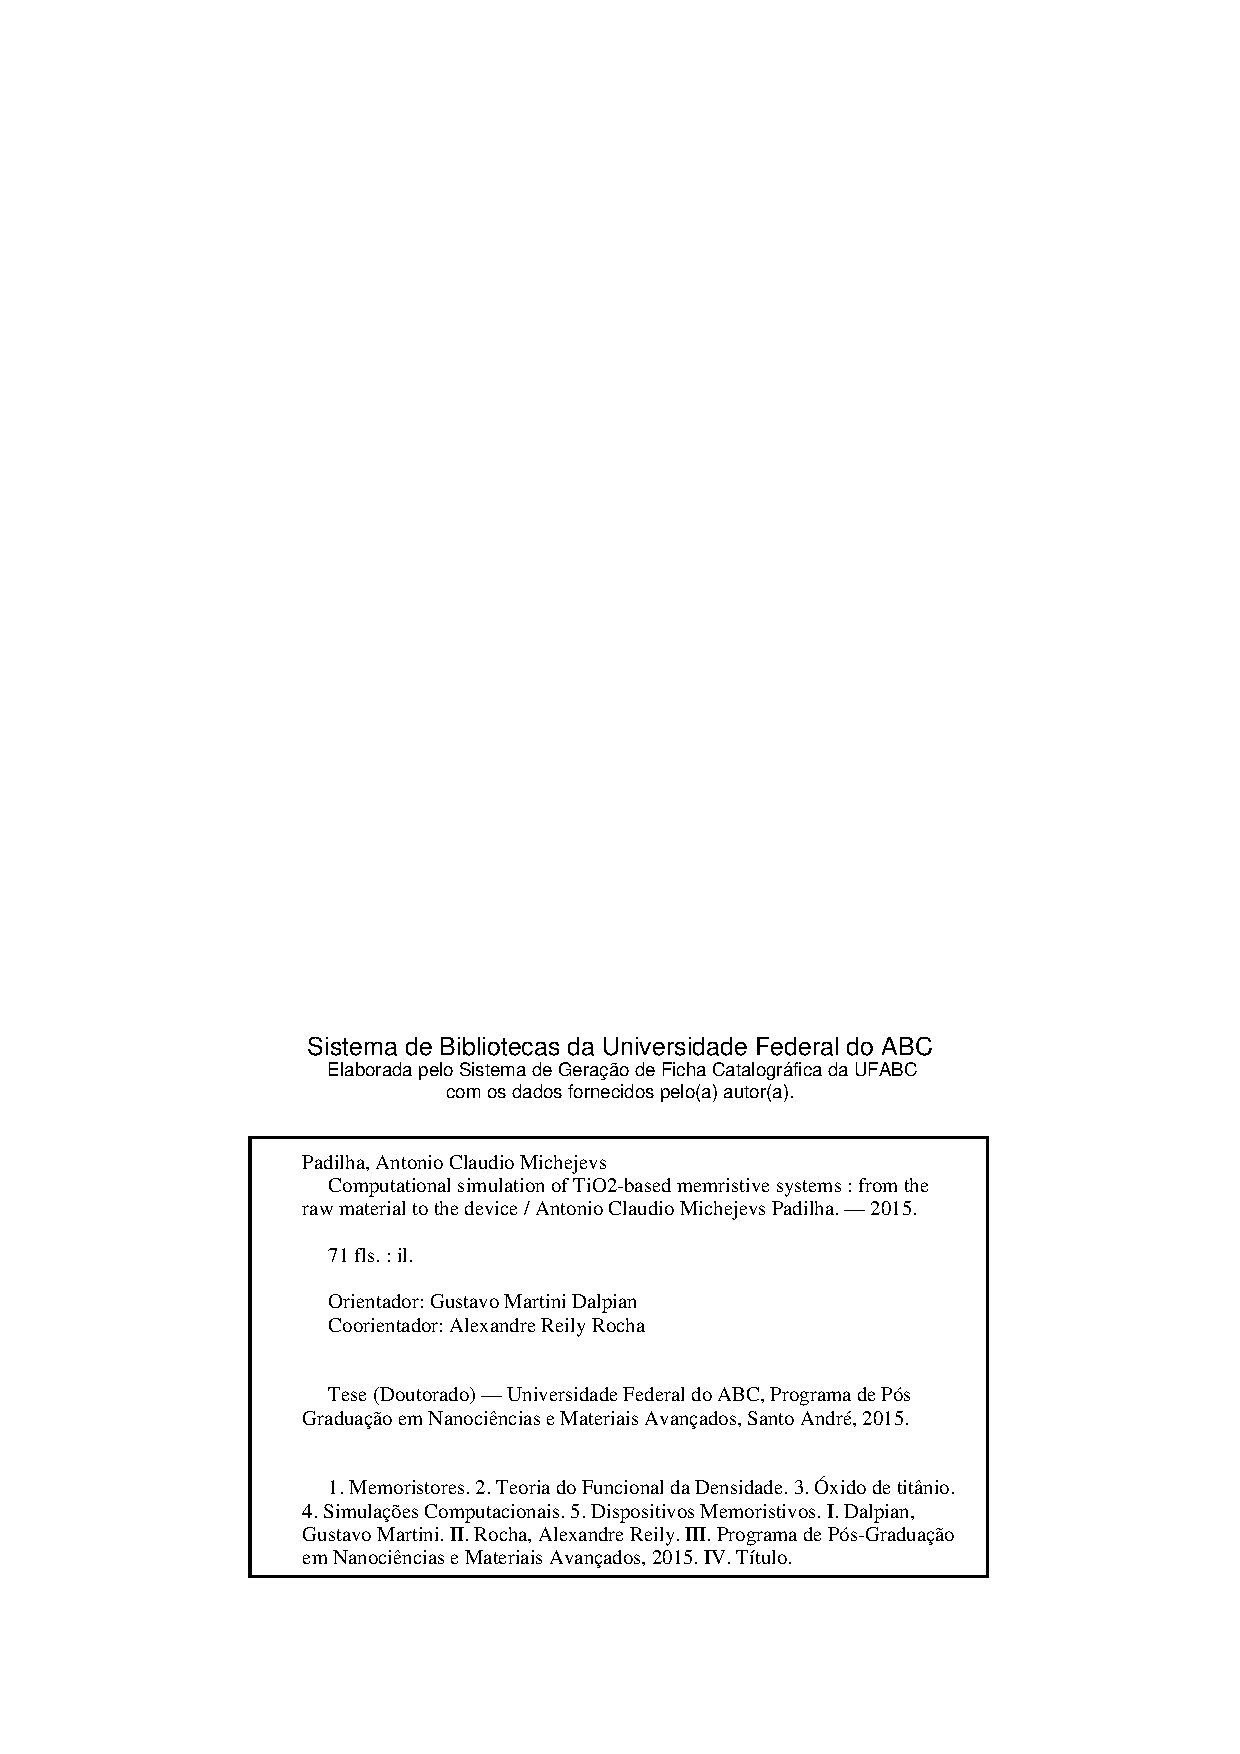
\includepdf[pages={-}]{burocracia/ficha-catalografica.pdf} %ficha catalografica

\newpage

\baselineskip 8.75 mm               %

% folha de assinaturas da banca
% USAR ORIGINAL NA VERSÃO IMPRESSA!!
\includepdf[pages={3}]{burocracia/Ata.pdf}

\newpage

% declaração de atendimento às observações da banca
% USAR ORIGINAL NA VERSÃO IMPRESSA!!
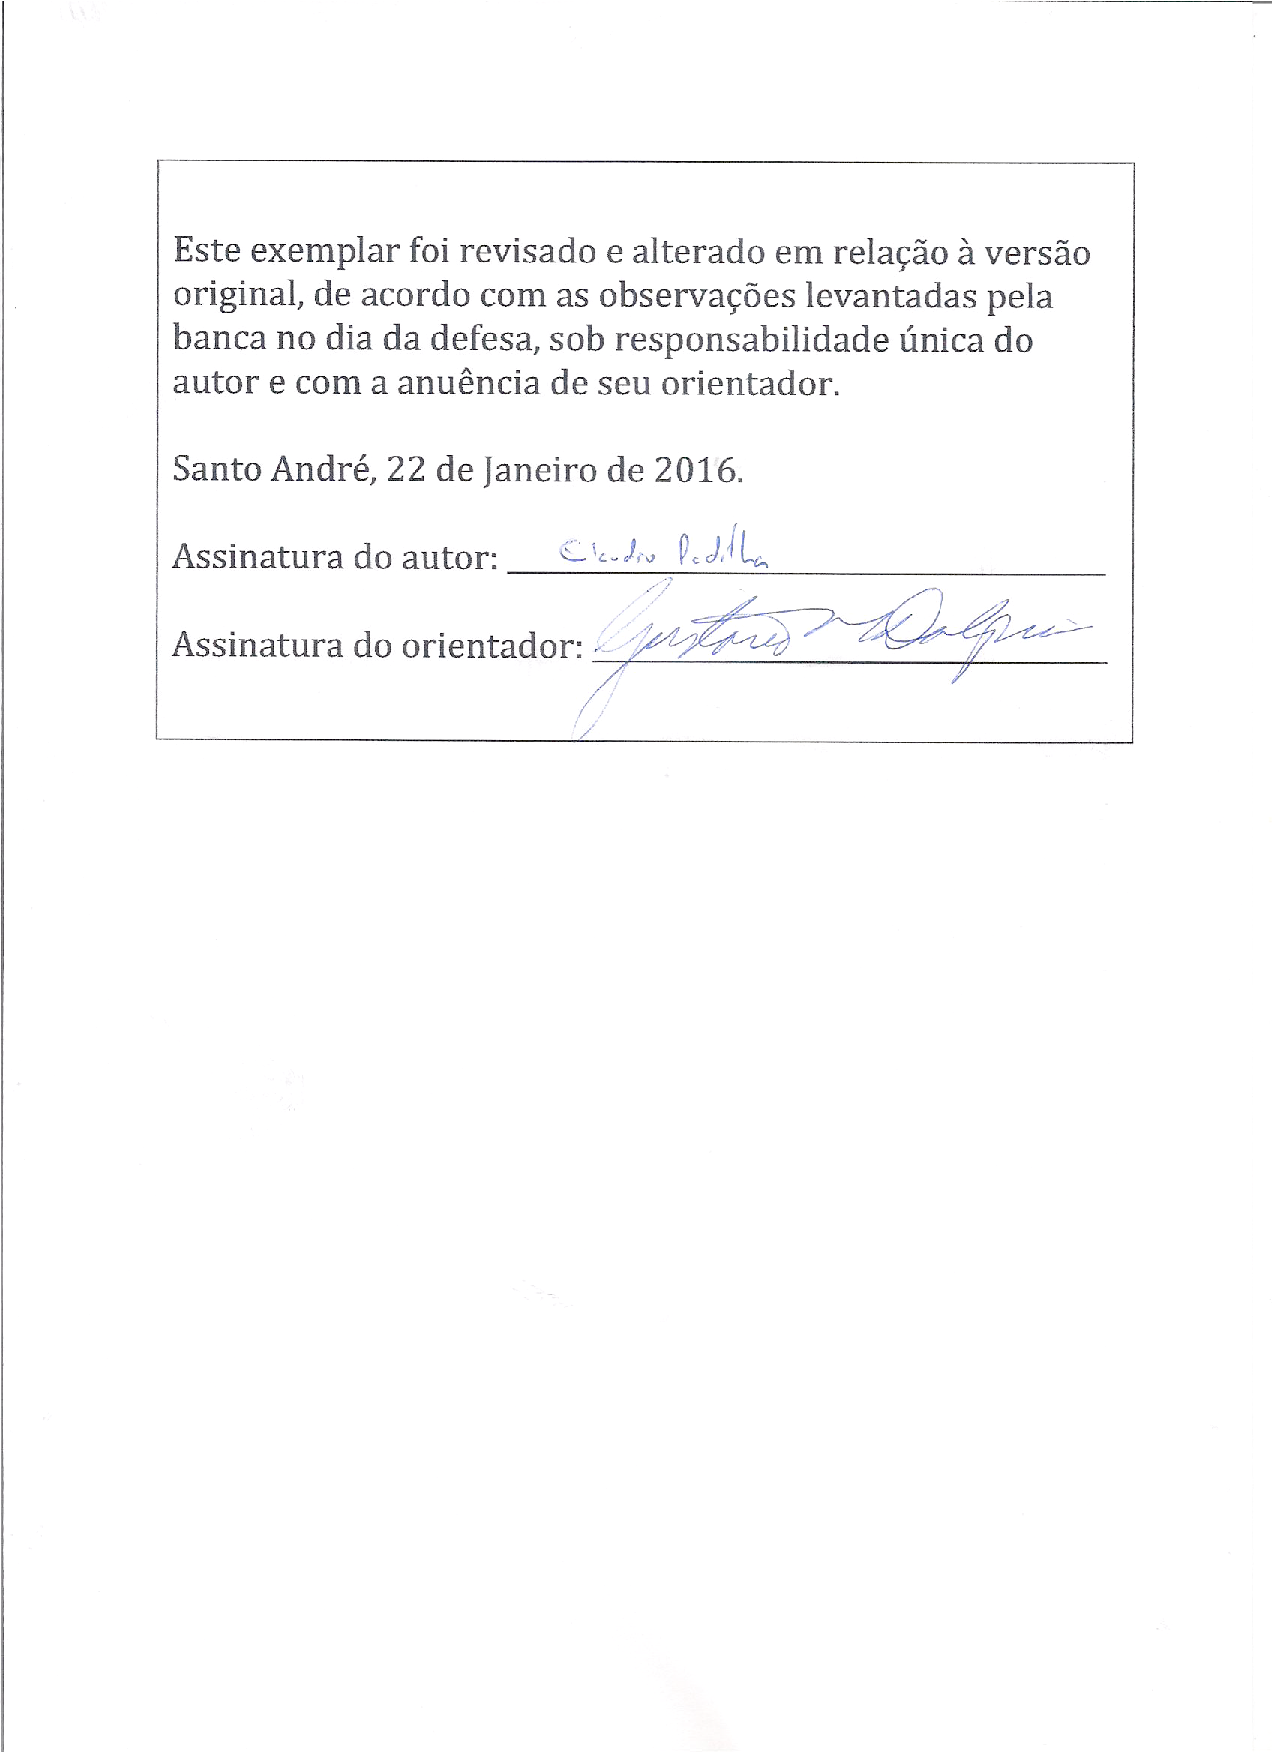
\includepdf[pages={-}]{burocracia/alteracoes-sign-200dpi.pdf}
                                    %
\thispagestyle{empty}               %
                                    %
\vspace*{-0.7cm}                    %

%%%%%%%%%%%%%%%%%%%%%%%%%%%%%%%%%%%%%%%%%%%%%%%%%%%%%%%%%%%%%%%%%%%%%%%%%%%%%%%%%%%%
%%%%%%%%%%%%%%%%%%%%%%%%%%%%%%%%%%%%%%%%%%%%%%%%%%%%%%%%%%%%%%%%%%%%%%%%%%%%%%%%%%%%
% Dedicatória =====================================================================%
\newpage
\thispagestyle{empty}

 \parbox{5.4in}{
  \begin{center}
   \begin{flushright}
    \textit{This thesis is dedicated to Vó Isaura \\ a brave Northeastern lady \\ whose greatest dream was to see her grandchildren as Doctors.}
   \end{flushright}
  \end{center}
 }

\frontmatter
\newpage
%\thispagestyle{empty}


%==================================================================================%

% Verso ===========================================================================%
% \vspace*{8cm}

% \hspace{3cm}\parbox[c]{20cm}{{\it The path is the goal.}}
% \vspace{0.7cm}

% \hspace{4cm}{\footnotesize Mahatma Gandhi}

% \thispagestyle{empty}
%==================================================================================%

% Agradecimentos ==================================================================%
\newpage
%\thispagestyle{empty}
%\frontmatter

\bigskip
\bigskip
\begin{center}
{\Large{\bf Acknowledgments}}
\end{center}
\vspace{1cm}

\begin{quote}
Now that the project is almost over, I can see how much of an adventure taking a PhD course is. Our lives can change significantly in four years, as the world we live in.

Four years ago I met two people that I never imagined would make such a difference in my life. Both my supervisor Gustavo Dalpian and my co-supervisor Alexandre Reily Rocha showed me how to make interesting and quality science and revealed me a whole world of opportunities as a scientist. Despite of all the problems we face in this business, I cannot recall them ever saying that the efforts are not worthy, and their example as professionals and human beings is something that I will try to follow in many aspects of my life. 

We geeks and nerds have evolved and at this point of history we (or most of us) are not lonely creatures anymore. I would like to thank all my friends and colleagues that in many times helped and taught me a lot of things, sometimes not only related to science, and sometimes not related to anything serious at all. This list can be very long, so taking the chronological order, thanks to Luiz Zenko for convincing me to go to UFABC, Aline Schoenhalz for being the "boss" of us all and helping me with my first steps using VASP, Rodrigo "Digão" Amorim for teaching me the fine art of tinkering and compiling, Jorge Osorio-Guillén also for teaching a lot about pseudopotentials and DFT methods, Patricia Sawamura and Leonard Kubben for hosting me in the US and being fantastic friends, and Hannes Raebiger, Lumico and Soungmin Bae for all the babysitting when I was in Yokohama. Many colleagues and friends I would like to acknowledge just for the time we spent together in L605, IFT, or SSMT: Alexandre Ramalho, Raphael Silva, Juan Camilo Alvarez, Douglas Baquião, Fábio Negreiros, Elierge Costa, Igor Dias, Ygor Jacques, Cleiton Maciel, Tancredo Fontinelles, Tarciso Filho, Antenor Neto, Alvaro Torrez, Luana Pedroza, Jeconias Guimarães, Wudmir Rojas, César "Kike" Villegas, Ekaterina Filatova, Pedro Brandimarte, Santiago Pérez-Walton, Camilo Valencia-Balvín, Daisuke Yoshida, Misaki Iwaya, Masamichi Kaiba, Takuma Munehiro, Kuniaki Ono, and Swasti and her lovely family.

Family plays a decisive part in all this. All support and love I received from my wife Sayuri was mandatory to arrive at this point with my sanity (more or less) preserved. My father Antonio, who never got tired of answering "but why?", and my mother Tatiana, who always supported me in my path with all her love, were also largely responsible for this achievement. The support both me and my wife received from my parents in law Eiko and Ikiyoshi should also be acknowledged. Finally, the most important person, the one responsible for the great part of my studies is my grandmother Isaura, who always told me that her mission would be fulfilled when both me and my brother Yuri were doctors. Thanks \textit{Vó Isaura}.

This work would not be possible without the financial support by São Paulo Research Foundation - FAPESP. The funding through grants 2011/21719-8, 2015/05830-7, 2010/16202-3, and 2011/19924-2 was paramount for my survival, participation in conferences, and acquisition of necessary equipment. The professionalism shown by FAPESP in all circumstances should be taken as an example. Another team that deserves this very same recognition is the staff at Cenapad-SP, where many calculations presented here were performed.

Of course there is always much more than I can fit here. From the bus drivers, cleaning staff, cafeteria staff, administrative staff, security staff, library staff, the people (still) building UFABC, and many other (many times invisible) workers, my thanks.
\end{quote}

\newpage
\hspace{1cm}
\newpage
%==================================================================================%
%%%%%%%%%%%%%%%%%%%%%%%%%%%%%%%%%%%%%%%%%%%%%%%%%%%%%%%%%%%%%%%%%%%%%%%%%%%%%%%%%%%%
            %dedicatórias, versos, agradecimentos
                                    %
%%%%%%%%%%%%%%%%%%%%%%%%%%%%%%%%%%%%%%%%%%%%%%%%%%%%%%%%%%%%%%%%%%%%%%%%%%%%%%%%%%%%

\newpage
%\thispagestyle{empty}
%\frontmatter
%==================================================================================%
\centerline{\large \textbf{Abstract}}

%\vspace{0.8cm}

\begin{quote}
The resistive switching or memristive property is the ability of a material to change its electrical resistance due to the application of an electric field. The memristor is a two-terminal device with this property that is capable of storing information as its resistance state, being architectured in a metal/insulator/metal stacking. This device can revolutionize the memory industry by providing fast switching and large retention times as well as high-density capabilities. However, its working principle is not completely understood at an atomic level, thus its application as next-generation resistive memories is hindered. Two mechanisms are proposed: ion drift mechanisms claim that the electric field and temperature gradients inside the device can form and dissolve a conducting filament, changing the electrical resistivity. On the other hand, electronic models consider charge trapping and de-trapping inside the insulator layer as the cause of the resistivity change. In this work we use a heuristic computational approach---density functional theory calculations and other numerical solutions---to understand the processes developing at the atomic scale inside TiO$_2$-based devices. Our results show that the oxygen deficiency in this material leads to the formation of a series of phases Ti$_n$O$_{2n-1}$ that present an intermediate band which can become charged when properly interfaced. The self-consistent-numerical solver of the Poisson equation shows multiple solutions that are related to the resistance states, and finally the potential is used in a transmission code that results in theoretical $i \times V$ curves for the memristor. \\ \textbf{Keywords:} Memristor, Memristive Devices, Density Functional Theory, DFT, Computational Simulation, Titanium Oxide, Magnéli Phases.
\end{quote}

\newpage

%%%%%%%%%%%%%%%%%%%%%%%%%%%%%%%%%%%%%%%%%%%%%%%%%%%%%%%%%%%%%%%%%%%%%%%%%%%%%%%%%%%%
\centerline{\large \textbf{Resumo}}

%\vspace{0.8cm}

\begin{quote}
A propriedade de chaveamento da resitência ou memoristiva é a habilidade de um material de alterar seu estado de resistência elétrica devido a um campo elétrico. O memoristor é um dispositivo de dois terminais com tal propriedade capaz de armazenar informação através de sua resistência, constituído de uma estrutura metal/isolante/metal. Este dispositivo pode revolucionar a indústria de memórias por apresentar tempos de chaveamento rápidos e de retenção longos, assim como altas densidades. Entretanto, seu princípio de funcionamento não é totalmente entendido a nível atômico, logo sua aplicação é impedida. Dois mecanismos são propostos: o mecanismo de difusão-deriva de íons afirma que campos elétricos e gradientes de temperatura formam e dissolvem canais condutores, alterando a resistividade. Por outro lado, modelos eletrônicos consideram o aprisionamento e liberação de cargas como causa da mudança da resistividade. Neste trabalho utilizamos uma abordagem heurística---cálculos de teoria do funcional da densidade e soluções numéricas---para entender os processos ocorrendo em escala atômica no interior de dispositivos baseados em TiO$_2$. Os resultados mostram que a dificência em oxigênio neste caso leva à formação de fases Ti$_n$O$_{2n-1}$ que apresentam uma banda intermediária, a qual pode se tornar carregada quando propriamente interfaceada. A resolução numérica da equação de Poisson apresenta múltiplas soluções relacionadas a diferentes estados de resistência, estas soluções são usadas em um código de transmissão que fornece curvas teóricas $i \times V$ para o memoristor. \\ \textbf{Palavras-chave:} Memoristores, Dispositivos Memoristivos, Teoria do Funcional da Densidade, DFT, Simulações Computacionais, Óxido de Titânio, Fases Magnéli.
\end{quote}

\newpage                  %resumo / abstract
                                    %
\tableofcontents                    %cria o índice automaticamente
\mainmatter                         %
                                    %
\chapter{Introduction}
\label{cap:intro}

Human history presents a series of important inventions that resulted in great advances to society. From the seemingly simple ones, such as the cart wheel, going through steam power, up to the transistor, most of the narrative is focused on the economic or social consequences of these inventions. The path that led from the scientific discoveries to the inventions, many of those being considered as the foundations of modern society, is, most of the time, not mentioned, perhaps because the application was straightforward or in some cases, the discovery was made by chance. The discovery of penicillin is one of the most famous of these cases \cite{Flemming1929}. 

Of course, in other cases the path was already set by theory, and what people today describe as an invention was the realization, in a controllable and predictable way, of one or more phenomena that were completely or partially understood at the time. The internal combustion engine and the steam-powered engine may be seen, from that point of view, as the biggest proofs of the success of thermodynamic theory, as well as the Bose-Einstein Condensates, which might enable quantum computing in the future \cite{Vinit2013}.

The pressure of society for solutions to many problems is another ingredient in this process, and lately the economic aspect of that pressure is the most obvious one. The semiconductor industry exemplifies that really well via Moore's law \cite{Moore1998}, which states that the number of transistors that can be built on top of a single integrated circuit roughly doubles each year. The reasons are not mainly due to technical advances, but mostly related to the cost of production. It is ironic that now we might have reached a limit for that law, due to the fact that devices cannot shrink beyond atomic sizes.

From the point of view of theory-driven inventions, one of the most interesting and promising ones is the case of the memristor. This new electronic device was proposed theoretically nearly 40 years ago \cite{Chua1971,Chua1976} but its realization was only claimed in 2008 \cite{Williams2008}. That realization brought many promises of a complete revolution in the computer business, but so far the device has not been completely understood, hence, its application is still not possible.

\section{Memristor: the missing circuit element}

In 1971, Leon O. Chua, using a symmetry argument, proposes the existence of a fourth fundamental circuit element, which he names the memristor \cite{Chua1971}. This new device would complete the set given by the known elements---resistor, capacitor, and inductor---in an elegant way: while the resistance may be interpreted as a quantity defining the relation between voltage $v$ and current $i$, the capacitor for the relation between charge $q$ and voltage $v$, and the inductor for the connection between magnetic flux $\varphi$ and current $i$, and taking into account the definition of current $(i=\nicefrac{dq}{dt})$ and Faraday's law $(v=\nicefrac{d\varphi}{dt})$, there would still be a missing relation: the one between the magnetic flux and charge. This relation is, thus, the definition of the memristor. The complete picture of these relations is shown on figure \ref{fig:circuit-elements}.

This new device is characterized by its memristance $M$, and the relation between the voltage and the current through the device was given by
\begin{equation}
  v(t) = M[q(t)]i(t),
  \label{eq:v_x_i_memristor}
\end{equation}
where the dependency of $M$ on $q$ can be easily shown if one uses the definition of current and Faraday's law on the relation between the magnetic flux and the charge\footnote{$v(t)=\frac{d \varphi}{d t} = \frac{d f}{d q} \frac{d q}{d t} = M[q(t)]i(t)$. Note that the explicit dependence on $q$ is only possible if the relation is not linear on $q$.} 
\begin{equation}
  \varphi=f(q).
  \label{eq:phi_x_q} 
\end{equation}

\begin{center}
  \begin{figure}[h!]
      \begin{center}
        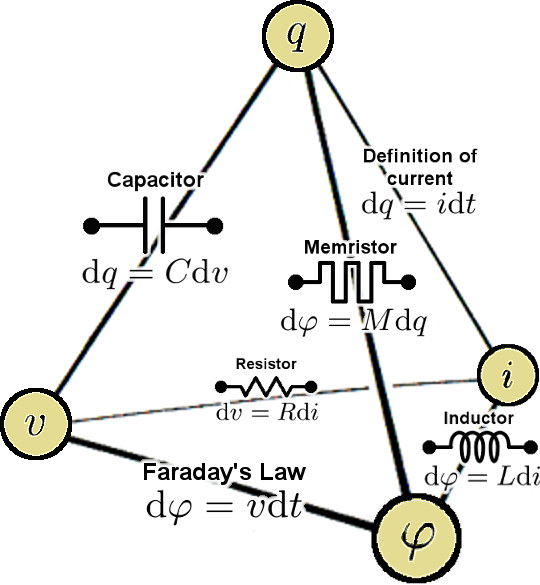
\includegraphics[width=0.5\textwidth]{img/memristor-vars.jpg}
        %\includegraphics[width=0.4\textwidth]{img/circuit-elements.jpg}
      \end{center}
      \caption{The four circuit elements and all relations between the fundamental circuit variables (charge $q$, voltage $v$, current $i$, and magnetic flux $\varphi$). At the edge that connects $q$ and $\varphi$ the symbol propoed by Chua for the memristor is depicted.}%At the bottom right square the symbol proposed by Chua for the memristor is depicted \cite{Williams2008}}.
      \label{fig:circuit-elements} 
  \end{figure}
\end{center}

According to Chua, the relation given by \ref{eq:v_x_i_memristor}, indicates that the memristance will depend on the amount of charge going through the device in a given time, {\em i. e.} this quantity will {\em remember} how much charge has passed by, and thus, the name memristor was proposed. Two examples of $i \times V$ curves obtained via equation \ref{eq:v_x_i_memristor} for different non-linear forms of equation \ref{eq:phi_x_q} are presented in Figure \ref{fig:lissajous-theo}. From those figures it is possible to extract two fundamental properties of Chua's memristor: i) the curves always cross themselves at the origin, meaning that no energy is stored in this device due to lack of delay between $i$ and $v$---usually referred to as {\em the pinched hysteresis loop} shape of the $i \times V$ curve---, and ii) that there are two possible slopes for the $i \times V$ curves at the origin, {\em i. e.} two values of electrical resistance.
\begin{center}
  \begin{figure}[h!]
    \begin{center}
      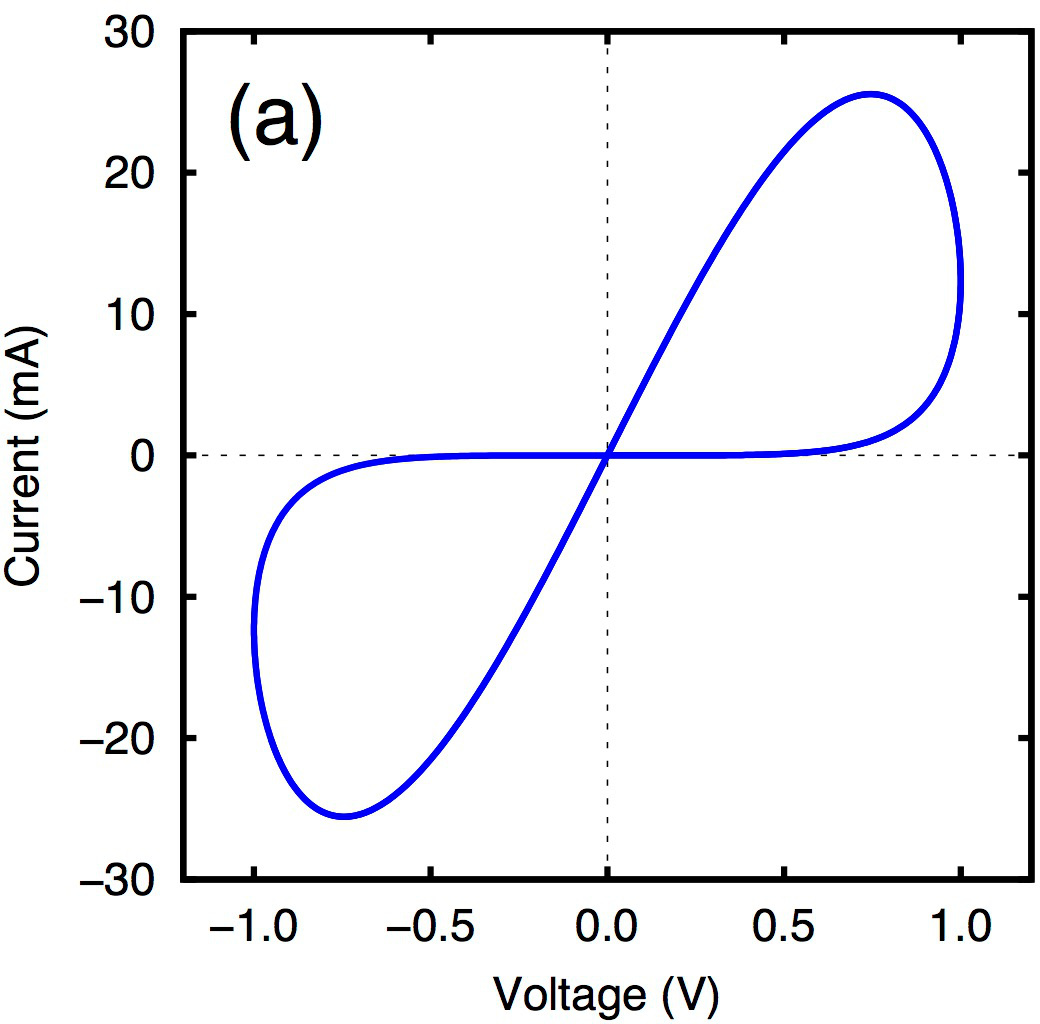
\includegraphics[height=6cm]{img/lissajous-01.jpg}
      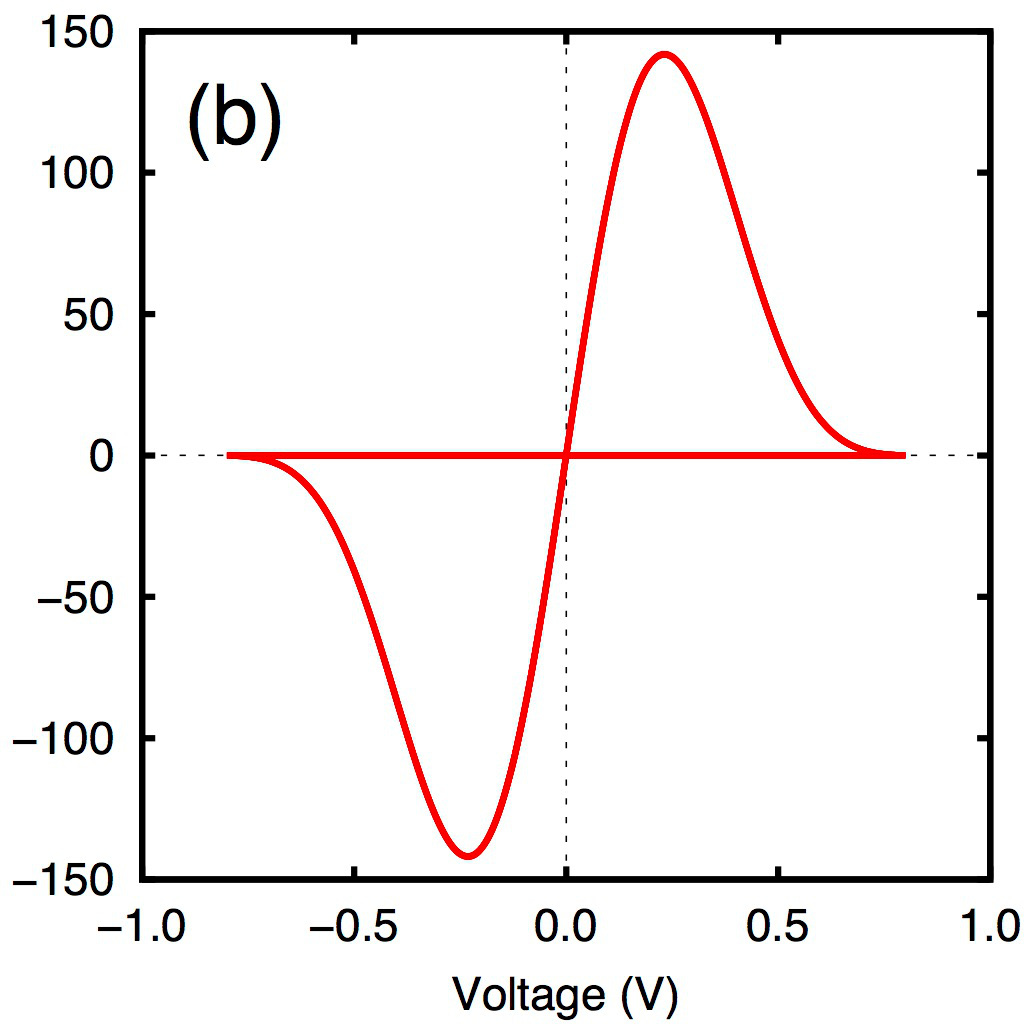
\includegraphics[height=6cm]{img/lissajous-02.jpg}
      \caption{Examples of $i \times V$ curves for (a) a third-order polynomial dependence of $\varphi$ on $q$ and (b) an exponential dependence.} 
      \label{fig:lissajous-theo} 
    \end{center}
  \end{figure}
\end{center}

A few years later, in 1976, Chua and Kang expanded the concept of memristor to a class of memristive systems \cite{Chua1976}. According to them, these devices are described by a set of equations,
\begin{align}
 v(t)&=R(x,i,t)i(t)\label{eq:memristive_devices_res} \\
 \frac{dx}{dt}&=f(x,i,t) \label{eq:memristive_devices_var}
\end{align}
where $x$ is a $n$-dimensional state vector which condensates all possible parameters that describe the state of the device, $f$ is a $n$-dimensional vector function and $R$ is a scalar continuous function. Explicit time-dependence is not mandatory for those quantities. In the particular case of the memristor, we have $x = q$, \(R(x,i,t) = M(q)\), and \(f(x,i,t) = \nicefrac{dq}{dt} = i\).

These two papers remained fairly unnoticed by the scientific community, and, until recently, this interesting theory was lacking its realization. Even though memory effects on thin films were reported throughout the 1970's, 80's, 90's and even at the beginning of the century \cite{Dearnaley1970,Pinto1971,Oxley1977,Hirose1976,Beck2000,Upadhyaya1995,Kim2006}, the connection of these results with Chua's theory was not noticed. This scenario was completely changed when an experimental group claimed they found the first memristor.

\section{The Missing Memristor Found}

In 2008, an experimental group led by Staley Williams at HP labs, working on resistance switching on thin films of titanium dioxide (TiO$_2$) claims the realization of Chua's memristor \cite{Williams2008}. A sketch of the device and the corresponding $i \times V$ curve obtained in their experiment is presented on figures \ref{fig:curva_hp_labs} (a) and (b). This realization of the memristor, as well as the following devices, is a two-terminal system where two metallic electrodes are separated by an active layer composed of a semiconductor or instulator thin film. Its $i \times V$ curve is such that both properties of memristor can be noticed: the crossing at the origin and the distinct low-bias resistances.
\begin{center}
  \begin{figure}[h!]
    \begin{center}
    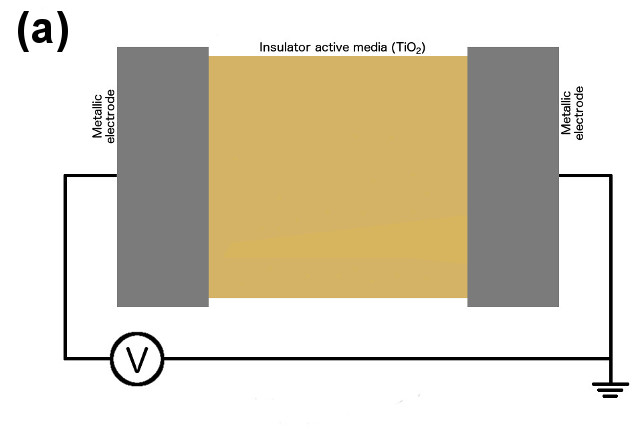
\includegraphics[height=6.2cm]{img/memristor-intro.jpg}
    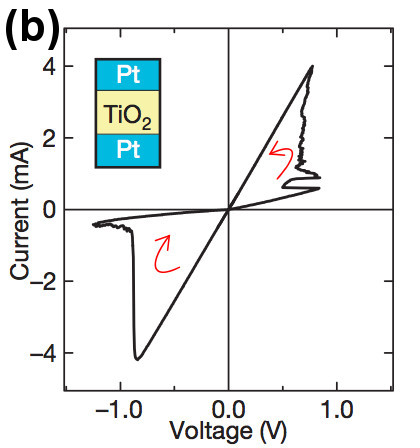
\includegraphics[height=6.2cm]{img/exp-HP.jpg}
      %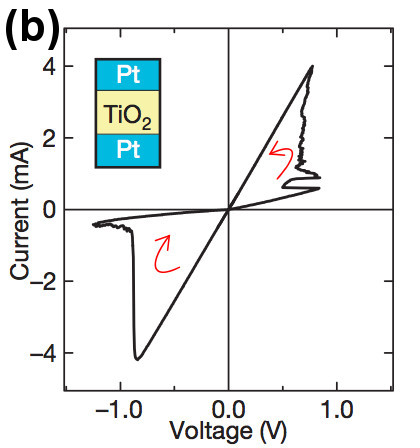
\includegraphics[width=0.7\textwidth]{img/exp-HP.jpg}
      \caption{(a) Schematic view of the TiO$_2$-based memristor. The voltage is applied at the opposing metallic electrodes throught the active layer. (b)Experimental $i \times V$ curve of a TiO$_2$-based memristor. The inset depicts the Metal/Insulator/Metal structure of the device\cite{Williams2008}.} 
      \label{fig:curva_hp_labs} 
    \end{center}
  \end{figure}
\end{center}

The model proposed by the authors considers the thin film as two one-dimensional resistors ($\mathcal{R}_{ON}$ and $\mathcal{R}_{OFF}$) connected in series and weighted by the width $w$ of the doped layer (the dopant being positively charged oxygen vacancies) of the semiconductor,
\begin{equation}
 v(t)=\left[\mathcal{R}_{ON}\frac{w(t)}{D}+\mathcal{R}_{OFF}\left(1-\frac{w(t)}{D}\right)\right]i(t),
 \label{eq:ohmic_hp_labs}
\end{equation}
where $D$ is the width of the thin film and consequently the upper boundary for $w$ ($0 \leq w \leq D$). The time evolution of $w$, {\em i. e.} the dynamics of the extent of the doped and undoped parts, is given by a phenomenological drift-diffusion model $\nicefrac{dw}{dt}= \mu_V E = \mu_V\left(\nicefrac{\mathcal{R}_{ON}}{D}\right)i(t)$, where $\mu_V$ is the dopant mobility and $E$ is the electric field, assumed constant across the device. Integration of this equation and substitution into equation \ref{eq:ohmic_hp_labs}, considering \(\mathcal{R}_{ON} \ll \mathcal{R}_{OFF}\), leads to
\begin{equation}
  v(t) = \mathcal{R}_{OFF}\left[1-\mu_V\frac{\mathcal{R}_{ON}}{D^2}q(t)\right]i(t)=M[q(t)]i(t).
  \label{eq:memristance_hp_labs}
\end{equation}

Due to the explicit dependence on $q(t)$ in \ref{eq:memristance_hp_labs}, this device is considered as the first realization of Chua's memristor. The explanation provided by the authors for the fact that nobody had never seen the realization of a memristor before was that people were not looking at the right scale: while the resistor, capacitor and inductor are feasible at the microscopic scale, the memristive property would be perceived only at the nanoscale ($D \sim 10^{-9}$ m). However, a recent historical review on memristors show that this might not be the case: gas-discharge tubes, tungsten filaments, high-pressure mercury-vapour lamps, among other macroscopic materials where a physical property presents inertia were reported to have the same characteristic $i \times V$ curves \cite{Prodromakis2012}.

As the time span between Chua's theoretical memristor and the experimental realization was nearly 40 years, the case of the memristor can be considered as a particular one: when although the theory was known, the realization was not at all simple.
\newpage

\section{Memristors and switching devices}

There was a sudden interest of the scientific community on the memristor after the paper from William's group in 2008. It happened not only because it was the first time one showed the equivalence between the memristor and the already known electric resistance switching devices, but also because the memristor brought a big promise for the computer memory industry. Those devices would be faster, denser, and less power-consuming than memory devices available today, mainly due to their smaller sizes and 3D stacking possibility (see reference \cite{Jeong2012} for a detailed comparison between memory technologies). 

In fact, the resistance switching property was already being investigated for quite some time, even before Chua's first paper on memristors. In 1965 Chopra obtains $i \times V$ curves for a series of oxides (Nb, Ta, and Ti) thin films sandwiched between metallic electrodes and detected a negative resistance when a threshold current was reached \cite{Chopra1965}. In 1968 Johnson observes unusual changes in TiO$_2$-rutile crystals' electrical resistance, which he attributed to the presence of H$^+$ impurities \cite{Johnson1968}. A recent historical compilation \cite{Prodromakis2012} shows that memristive phenomena have been detected for the last two centuries, even before the discovery of the other electronic devices such as the resistor, capacitor, and inductor. Many authors report unexpected behaviors for the electrical resistance of oxides, from the early 60's until quite recently before the William's group claim \cite{Hickmott1962,Argall1968,Oxley1977,Hirose1976,Upadhyaya1995,Beck2000,Waser2007}, but none of them could point out the link between their results and Chua's theory. There is even a model, older than Chua's, for resistance switching, given in a 1967 paper by Simmons and Verderber \cite{Simmons1967} where they study resistance switching in silicon oxide thin films containing gold impurities, but it has drawn very little attention. This lack of interest can be understood from the technological scenario of that time, where silicon integrated circuits were becoming the work horse of the computer industry and remained undisputed until the end of the 90's, when people realized that Moore's law \cite{Moore1998} could not be sustained in the long run.

Of course, not all feedback is positive to William's group paper. A few authors questioned whether the realization of the memristor was actually a discovery or just a claim looking for huge impact and consequently huge profits. Among those, we can identify some interesting arguing whether the memristor and the resistance switching devices are the same thing or not \cite{Gale2014}. One of the main points against William's group claim and the equivalence between memristors and switching devices is that while the first is defined by Chua's theory from electromagnetic theory---and the crucial point is that it explicitly includes magnetism in its mathematical derivation---, the switching devices proposed mechanisms, so far, do not rely on that. Leon Chua himself has given his opinion recently, stating that "Resistance switching memories are memristors" \cite{Chua2011} and "If it's pinched it's a memristor" \cite{Chua2014}. His point is that the required properties for a device to be considered a memristor are given by its $i \times V$ curve characteristics---a pinched hysteresis shape is the memristor's fingerprint---, which are fullfiled by the switching devices. He even presents a general differential equation to define the state vector (as defined by equation \ref{eq:memristive_devices_var}) of a memristor in terms of power series,
\begin{equation}
  \frac{dx}{dt} = \sum_{i=1}^m a_i x^i + \sum_{j=1}^n b_j i^j + \sum_{j,k=1}^{p,r} c_{jk} x^j i^k
  \label{eq:chua_2011}
\end{equation}
where the careful choice of the parameters \(\{a_i, b_i, c_{ij}\}\) would be enough to fit any experimental $i \times V$ curve of a memristor. For instance, the HP memristor model is described by \(x = w(t)\) and \(a_i = c_{ij} = 0\), \(b_1 = \mu_V \left(\nicefrac{\mathcal{R}_{ON}}{D}\right)\), and \(b_i = 0\) for \(i>1\). Despite the discussion between supporters and deniers of the equivalence between these devices, many authors today use both terms interchangeably \cite{Yang2012,Waser2009,Szot2011,Strachan2009}, which means that the first group is the larger one. I adopt the same position in this thesis, thus, from this point on the names {\em memristor} and {\em resistance switching device} or just {\em switching device} will be used indistinctly to refer to the same system. 

In a general way, memristors are composed of a thin insulator film---usually referred to as the active media---sandwiched between two electrodes. Some of the materials used as active media are binary oxides (TiO$_2$ \cite{Choi2005,Hickmott1962,Argall1968,Kim2013c,Yang2011,Miao2011b,Williams2008}, Ta$_2$O$_5$ \cite{Pinto1971,Hickmott1962,Miao2011a,Beck2000}, TaO$_x$ \cite{Yang2010,Miao2012}, Nb$_2$O$_5$ \cite{Pinto1971,Kundozerova2012}, NiO \cite{Seo2004,Wang2013}, ZnO \cite{Huang2013,Chen2013}, SiO \cite{Simmons1967,Hickmott1962,Chang2013}, Al$_2$O$_3$ \cite{Hickmott1962}, ZrO$_2$ \cite{Hickmott1962,Kim2013b}, HfO$_2$ \cite{Syu2013,Luo2013}, Fe$_2$O$_3$ \cite{Kim2013a}, and WO$_3$ \cite{He2013}), perovskites (PbTiO$_3$ \cite{Pilch2014}, SrTiO$_3$ \cite{Muenstermann2010,Szot2006}, SrZrO$_3$ \cite{Beck2000,Rossel2001,Guo2013}, (Pr,Ca)MnO$_3$ \cite{Ignatiev2006}, (Sm,Ca)MnO$_3$/(La,Sr)MnO$_3$ \cite{Sawa2006}), silicon \cite{Dong2008,Mehonic2012}, and other systems as sulfides (Ag$_2$S$_3$ \cite{Hirose1976}, (Zn,Cd)S \cite{VanderSluis2003}), carbon-based systems (C$_{60}$, C$_{70}$, and C$_{84}$ encapsulated inside double-walled carbon nanotubes \cite{Li2009}), and polymers (poly-spirofluorene \cite{Gomes2008}). Electrode materials comprise a wide range of metals as Au \cite{Chopra1965,Hickmott1962,Beck2000}, Ag \cite{Chopra1965}, Al \cite{Chopra1965,Choi2005,Hickmott1962}, Pt \cite{Kim2013b,Choi2005,Miao2011a,Beck2000,Yang2010,Miao2012,Huang2013,Chen2013}, Ru \cite{Choi2005}, Ta \cite{Hickmott1962,Miao2011a,Yang2010,Miao2012}, Zr \cite{Hickmott1962}, Ti \cite{Hickmott1962,Syu2013}, Cu \cite{Waser2009}, TiN \cite{Kim2013b,Syu2013}, and many other materials (see ref. \cite{Pan2014} and references therein). A key point that binds all these materials in the large group of memristive materials is that for all cases defects are present in the materials, either in the form of point defects in a crystalline system, or by use of amorphous thin films.

\begin{center}
  \begin{figure}[h!]
    \begin{center}

      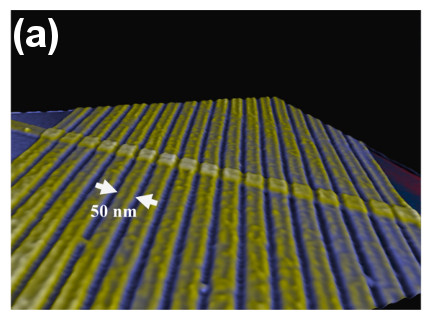
\includegraphics[height=5.5cm]{img/MiaoNanotechnology2011.jpg}
      %\includegraphics[height=5.5cm]{img/memristor.jpg}
      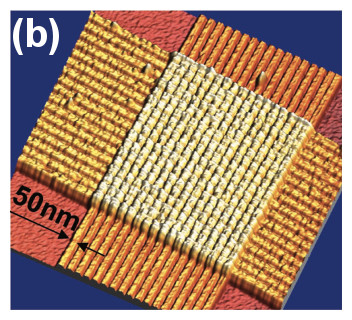
\includegraphics[height=5.5cm]{img/MiaoAdvMat2011.jpg}
      %\includegraphics[height=3.6cm]{img/YangAPL2012.jpg}
      \caption{Atomic force microscopy image of a crossbar junction network of (a) TaO-based \cite{Miao2011a} and (b) TiO$_2$-based memristors \cite{Miao2011b}.} 
      \label{fig:sketch-mem} 
    \end{center}
  \end{figure}
\end{center}

The memristor's two-terminal device spatial arrangement is obtained using lithography for the metallic layers and many deposition methods for the active layer, as sputtering \cite{Miao2011b}, pulsed laser deposition \cite{Muenstermann2010}, low-pressure chemical vapor deposition \cite{Chang2013}, and by oxidation of the bottom electrode \cite{Jeong2012}. One important detail is that none of those techniques yield perfect crystals: defects are always present. For high-density memories, the memristor cells are structured in a crossbar junction network, as shown in Figures \ref{fig:sketch-mem} (a) and (b), where each electrode crossing enclosures a memristor.

\begin{center}
  \begin{figure}[h!]
    \begin{center}
      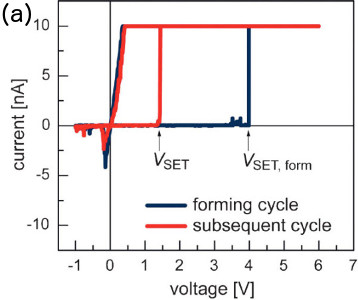
\includegraphics[height=4.1cm]{img/Wasser2009-electroform.jpg}
      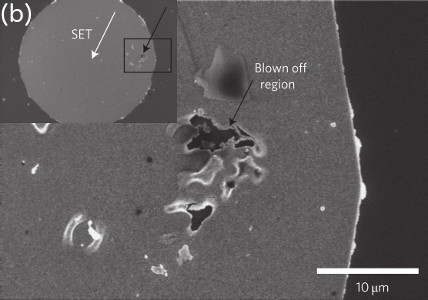
\includegraphics[height=4.1cm]{img/Kwon2010NatureNanoBolhas.jpg}
      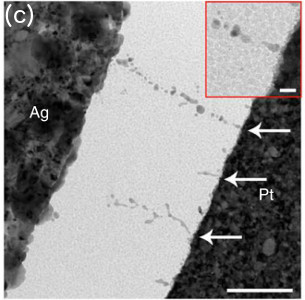
\includegraphics[height=4.1cm]{img/Yang2012NatureCommCanais.jpg}
      \caption{(a) $i \times V$ curve for a Cu/SiO$_2$/Pt memristor where the forming cycle and subsequent cycles are depicted \cite{Waser2009}. The constant current of 10 nA is the compliance current. (b) Scanning Electron Microscope (SEM) image of the blown-off region of top-electrode of a Pt/TiO$_2$/Pt device \cite{Miao2011a}. This result is explained by the formation of O$_2$ under this electrode after the electroforming. (c) Ag channels formed after electroforming step on top of a planar Ag/SiO$_2$/Pt device \cite{Yang2012}. Scale bar is 200 nm.} 
      \label{fig:electroform-channel} 
    \end{center}
  \end{figure}
\end{center}

After the process of structurally building the device, an electroforming step is required for the majority of the reported systems to properly switch. This process consists of a soft breakdown of the dielectric, which is performed by subjecting the pristine device to a voltage larger than usual switching voltage, keeping the resulting current bounded by the so-called compliance current (see fig. \ref{fig:electroform-channel}). At a microscopic level, it is believed to result in local heating and filamentary conduction before structural changes take place in the active media due to ionic migration \cite{Sharma2014,Yalon2012}. The main consequence of such process is the introduction of defects in the active media, such as oxygen vacancies---evidenced by the escape of O$_2$ gas from oxides \cite{Kwon2010,Jeong2012,Chen2013,Miao2011a}---or metal impurities---usually due to ionic migration of Cu$^+$ and Ag$^+$ species from the electrodes into the active media \cite{Yang2012,Yang2014,Guo2007}. Experimental data for both cases is presented in figure \ref{fig:electroform-channel}.

The devices after electroforming can store information via its switcheable resistance state. In order to write information, a voltage beyond a threshold value is required and this process can take place in two modes: unipolar or bipolar. In the unipolar mode, the switching from a high-resistance state (HRS) to a low-resistance state (LRS) (usually referred to as the reset process) and the other way around (the set process) can be performed using the same polarity of the applied voltage. On the other hand, devices operating in the bipolar regime are set and reset using different polarities. These two modes of operation are illustrated in figure \ref{fig:unipolar-bipolar}. The read operation is performed using a small bias, such that the system is not disturbed from its current resistance state.

Current devices show a great promise for future memory technologies. Switching times as fast as picoseconds and $\mathcal{R}_{ON}/\mathcal{R}_{OFF}$ ratios higher than 10$^9$ have been reported \cite{Pan2014}. Another important feature is the number of read/write cycles a device can stand, which is usually referred to as the endurance. For TaO-based devices, up to 10$^9$ reliable cycles have been reported \cite{Yang2010}. Due to the fact that once the system is set or reset the lifetime of programmed state is stable for years \cite{Lee2011,Waser2007}, the memristor also presents the potential to unify the volatile (such as random access memories - RAM) and non-volatile memories (magnetic media, flash). This new device shows the best attributes of the latter, as fast switching times and low power consumption, and of the former, as long retention times and large number of read/write cycles. For a comparison with other technologies such as RAM and flash, a comprehensive review is presented by Jeong {\em et al.} \cite{Jeong2012} as well as others \cite{Fujisaki2010, Chua2011, Kim2011, Waser2007, Waser2009, Yang2012, Szot2011, Pan2014}.

\begin{center}
  \begin{figure}[h!]
    \begin{center}
      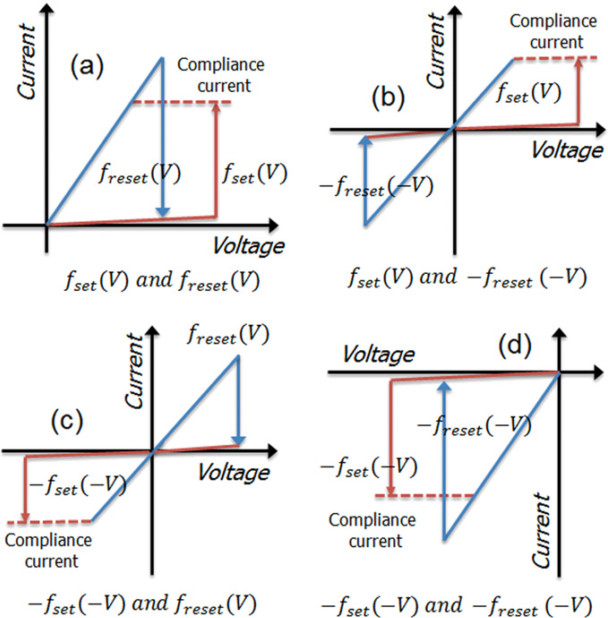
\includegraphics[height=11cm]{img/Jeong2012RepProgPhys.jpg}
      \caption{Schematic $i \times V$ curves for memristors. In (a) and (d) one sees unipolar switching while in (b) and (c) the bipolar regime is shown. $f_{\text{set}}$ and $f_{\text{reset}}$ are the sections of the $i \times V$ curves related to each process \cite{Jeong2012}.}
      \label{fig:unipolar-bipolar} 
    \end{center}
  \end{figure}
\end{center}

Even though the memristor presents remarkable properties for next-generation memory technologies, its immediate application is hindered by the lack of understanding of the working principle at a microscopic scale. For example, the switching time presents a strong non-linear dependency with respect to the applied voltage, which in turn leads to statistical variation of that time \cite{Medeiros-Ribeiro2011,Pickett2009}, making it very difficult to efficiently operate the device in a controlled fashion. Another important point is that the memristive property arises in a wide range of systems, thus suggesting that either the working principle is not material-related or it has a variety of diferent origins.
\newpage

\section{Models}
\label{sec:models}

Given the current scenario, many models were proposed to explain these promising devices, and two of them could be considered the best accepted so far: ionic drift-diffusion and purely electronic models. As explained earlier, the electroforming process is responsible for introducing a number of defects inside the active layer, which in turn may acquire the shape of a channel, as shown in Figures \ref{fig:electroform-channel} (c) and \ref{fig:canais-TiO}. The ionic model states that these channels will short circuit the device (span the whole device width, connecting both electrodes) while in the ON state, and a small part of that channel will be removed increasing the resistance of the device into the OFF state once the polarity is reversed or due to Joule heating in the unipolar case \cite{Pickett2009}. The fast switching times are made compatible with this model by assuming that the diffusion barriers for ions inside the active material can be lowered by presence of large electric fields and/or high temperature spots. This picture is known in the literature as the field/temperature enhanced acceleration of ionic movement \cite{Ielmini2012,Ielmini2011}.
\begin{center}
  \begin{figure}[h!]
    \begin{center}
      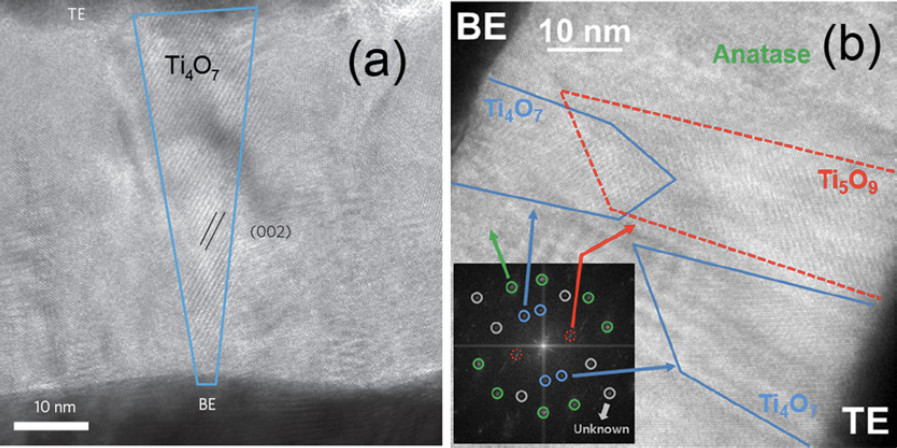
\includegraphics[width=12cm]{img/Jeong2012canaisTiO.jpg}
      \caption{Transmission Electron Microscope (TEM) images of (a) single Ti$_4$O$_7$ channel \cite{Kwon2010} and (b) multiple Ti$_4$O$_7$ and Ti$_5$O$_9$ channels \cite{HwanKim2011} inside TiO-based memristors. The inset in (b) shows X-ray diffraction data used to characterize the different parts of the active region.} 
      \label{fig:canais-TiO} 
    \end{center}
  \end{figure}
\end{center}

On the other hand, purely electronic models, which can be tracked down to the late 60's, explain the switching phenomena mainly according to the trapping and de-trapping of charges inside the active region due to the presence of intrinsic or extrinsic impurities \cite{Simmons1967}. Other less popular electronic models claim that the switching is caused by metal/insulator Mott transitions \cite{Stoliar2013,Yalishev2012} or modulation of the Schottky barrier \cite{Marchewka2015}. In any of those cases, there is an apparent dilemma from the energetic point of view: if the LHR and HRS are electronic by nature, there may be a potential barrier that separate those states. Such barrier should be low enough that the switching time is fast but in order for the final states to be stable, the same barrier should be high. This picture is referred to as the "voltage-time dilemma" by Schroeder {\em et al.} \cite{Schroeder2010}. The main issue in this work is that the authors assume a solution to the Poisson equation and give an {\em ansatz} solution as the potential energy barrier for electrons injected into the active media ({\em i. e.} the conduction band minimum - CBM) but do not solve it. As I will show, it is possible to overcome the voltage-time dilemma by performing a self-consistent calculation that treats the problem in a more realistic fashion.

Summarizing, even though many experimental results point out the existence of filaments inside the active region of the devices, there is no direct proof of the filament formation and subsequent dissolution within the timescale reported for the switching process. The electronic models however, were not throught explored, and theoretical and/or computational studies are scarce. An atomic scale picture of the memristor is still missing, even though it is a consensus that the understanding of the processes taking place at this scale is the key to unravel the memristor. Questions as why the device switches so fast and at the same time stores information for such a long time, or how unipolar switchin works, or even why the memristive property is observed in so many materials that, in principle, present no simmilarities at all, are still waiting for definite answers.

\section{The contribution of this work}
\label{sec:contrib}

Our contribution is to understand the memristor from a theoretical point of view. As most of the data on memristors was obtained experimentally---and thus via indirect measurements---, it is currently very difficult to understand the processes taking place inside the devices during switching. Even the properties of the nanometric structures formed inside the devices are not completely known. In this scenario, density functional theory (DFT) calculations are already proven to be a viable and powerfull tool able to probe the atomic-level interactions within a nanoscale system. The fast developement of numerical algorithms and hardware, as well as of the theory itself, has enabled the spread of many DFT-based electronic structure codes in the last two decades \cite{Becke2014,Capelle2006}.

The choice of focusing on TiO$_2$-based devices is twofold: i) it is one of the most popular materials for devices manufacturing \cite{Szot2011,Gale2014,Jeong2012,Miao2011b}, as is the case of the prototypical device developed by HP \cite{Williams2008}, and ii) the intrinsic defects, oxygen vacancies and titanium interstitials are known to present stable charge states \cite{Janotti2010,Lee2012} within the bandgap. Within ion-drift models, this last feature is considered only due to the action of the electric field on charged vacancies \cite{Strukov2009,Williams2008,Kwon2010}, but no recent reports on the changes of the properties of these materials upon charging and de-charging are available.

One of the first steps in any study is to choose one or more methodologies out of many. As it is known in the electronic structure community, DFT is based on an approximation for the exchange and correlation contributions to the total energy of the system \cite{Capelle2006,Becke2014}. The ground state total energy of a quantum system composed by $n$ interacting electrons subject to an external potential is a functional of the ground state electronic density within this theory. There are many levels of approximation that can be used and several ways to express this functional dependecy, the key difference is how the \textit{exchange} and \textit{correlation functionals}\footnote{From now on we will refer to the \textit{exchange} and \textit{correlation functionals} used simply as \textit{functionals}} are written given a degree of the approximation. The accuracy and suitability of the different functionals when used for specific systems should always be probed in these kinds of studies. With that in mind, our first work was to compare three different functionals: the local density approximation (LDA) \cite{Ceperley1980}, the generalized-gradient-approach (GGA) functional proposed by Perdew, Burke and Ernzerhof (PBE) \cite{Perdew1997} parametrized for better description of solids and surfaces (PBESol) \cite{Perdew2008}, the same functional with the on-site Hubbard $U$ parameter for $d$ electrons \cite{Dudarev1998} and the screened hybrid functional by Heyd, Scuseria and Ernzerhof (HSE) \cite{Heyd2003}. This study was performed for TiO$_2$ and its oxygen-deficient phases known as the Mangéli phases---present inside the TiO-based memristors after electroforming---and is presented in chapter \ref{chap:raw}.

The next question that naturally arose was how the oxygen-deficient phases interact electronically with the surrounding TiO$_2$ matrix. To answer that question, the band offset between TiO$_2$-rutile and the Magnéli phase Ti$_4$O$_7$ was obtained and is presented in chapter \ref{chap:band-offset}. To achieve this goal, a supercell approach was employed, and using crystallographic operations the Magnéli structure was derived from the rutile one, making it possible to match the structures without any stress on the interface.

Another key point was the stability of the oxygen-deficient phases. Some studies already pointed out that the Magnéli phases are more stable than the rutile structure containing some ammount of defects---either oxygen vacancies or titanium insterstitials---that mimics their non-stoichiometric composition \cite{Liborio2008}, but the exchange of electrons with the electrodes was not taken into account. We performed thermodynamical calculations to asses the stability of Ti$_2$O$_3$, Ti$_4$O$_7$, and Ti$_5$O$_9$ in such situation. Our results, reported in chapter \ref{chap:charges}, indicated that these systems could in principle store positive charges in a similar way to what happens when point defects are present inside insulators or semiconductors. This charging and de-charging process could change the electronic transport mechanism in those systems and thus enable electronic switching.

The last part of this work was to solve the Poisson equation for the memristors. This was performed using the code developed in collaboration with Dr. Hannes Raebiger from Yokohama National University, while he was working as a visiting professor at UFABC. The numerical results shown in chapter \ref{chap:bandbend} pointed out the possibility of an electronic mechanism for switching, based on deffect-assisted charge trapping inside the active media. Multiple solutions of the Poisson equation were interpreted as diferent resistance states, as each one reveals the true profile of the barrier for incoming electrons in memristors. 

%The contribution of this work is to understand the memristor from a theoretical point of view. Using density functional theory (DFT) calculations for TiO$_2$---one of the most popular materials used to build memristors---and its oxygen-deficient phases known as the Mangéli phases---present inside the TiO-based memristors after electroforming---, we could understand the properties of those materials at atomic level and evaluate their energy band alignment at the interfaces. The stability of the Magnéli phases was studied from the point of view of thermodynamic total-energy calculations when the system is allowed to exchange atoms and electrons with reservoirs. The role of charging and de-charging of electron traps was elucidated and numerical solutions of the Poisson equation were obtained, revealing the true profile of the barrier for electrons in memristors. 		          %chap 1
\chapter{Raw Materials}
\label{chap:raw}

The prototypical memristor was based on a titanium dioxide thin film sandwiched between metallic electrodes \cite{Williams2008}, and many other devices have been manufactured by following the same recipe \cite{Szot2011,Kwon2010,Jeong2012,Pan2014}. Experimental data shows that oxygen-deficient phases of TiO$_2$ are formed inside the oxide layer of these devices \cite{Kwon2010,HwanKim2011}. For this reason, we start our bottom-up study of the devices by investigating the electronic structure of the non-stoichiometric compounds known as the Magnéli phases (Ti$_n$O$_{2n-1}$, $n = 4, 5$) as well as the Ti$_2$O$_3$-corundum structure and the $\alpha-$, $\beta-$, and $\gamma-$ phases of Ti$_3$O$_5$. 

\begin{center}
 \begin{table}[h!]
  \centering
   \caption{\label{tab:symm} International and Schoenflies notations for the space groups of TiO$_2$-rutile, and Ti${}_n$O${}_{2n-1}$, ($2 \leq n \leq 5$) \cite{Belsky2002,Aroyo2006}.}
   \begin{tabular}{p{0.2\columnwidth}p{0.3\columnwidth}p{0.2\columnwidth}} 
   \hhline{===}
                              & \multicolumn{2}{c}{Space Group}    \\
                              & International (\#) &  Schoenflies  \\
    \hline
    TiO$_2$-rutile			  & $P4_2/mnm$ (136)   & $D_{4h}$      \\
    Ti${}_2$O${}_3$           & $R\bar{3}c$ (167)  & $D_{3d}$      \\
    $\alpha$-Ti${}_3$O${}_5$  & $Cmcm$ (63)        & $D_{2h}$      \\
    $\beta$-Ti${}_3$O${}_5$   & $C2/m$ (12)        & $C_{2h}$      \\
    $\gamma$-Ti${}_3$O${}_5$  & $C2/c$ (15)        & $C_{2h}$      \\
    Ti${}_4$O${}_7$           & $P\bar{1}$ (2)     & $C_i$         \\
    Ti${}_5$O${}_9$           & $P1$ (1)           & $C_1$  \\ 
    \hhline{===}
   \end{tabular}
 \end{table}
\end{center}

Table \ref{tab:symm} presents the space groups of the systems studied at this stage. The structures present larger unit cells as $n$ in Ti$_n$O$_{2n-1}$ becomes larger. In fact, the larger the value of $n$, the closer to stoichiometric TiO$_2$: for $n > 37$ the structure is rutile with point defects or Wadsley defects \cite{Szot2011}. On the other hand, for smaller values of $n$, the formation of new structures was reported by Andersson and Magnéli \cite{Andersson1957}.

For all systems the equilibrium lattice constants and ion positions were obtained via DFT calculations. Two approximations were used for the exchange-correlation functional: GGA approximation via PBESol functional and screened hybrid as implemented in HSE. The relaxation output data is presented in the table \ref{tab:struct-relax-prb}. The error in comparison with experimental data from X-ray diffraction spectra was considered small, being the highest deviation for $\alpha$-Ti$_3$O$_5$ close to 6\% with respect to unit cell volume. Further details of the parameters used in all calculations can be found in appendix \ref{sec:app-calc}.
 \begin{table*}[ht!]
  \centering
  \caption{\label{tab:struct-relax-prb} Experimental and theoretical values of lattice parameters for the Ti${}_2$O${}_3$, $\alpha-$, $\beta-$ and $\gamma$-Ti${}_3$O${}_5$, Ti${}_4$O${}_7$, and Ti${}_5$O${}_9$ structures. Mean Absolute Relative Error for unit cell volume is also presented in parenthesis. Values presented are those of the primitive cells.}
   \begin{tabular}{*{2}{p{0.012\textwidth}} p{0.14\textwidth} *{3}{p{0.06\textwidth}} *{3}{p{0.07\textwidth}} *{1}{p{0.18\textwidth}}} 
  \hhline{==========}
       &               &                          & $a$(\AA) & $b$(\AA) & $c$(\AA) & $\alpha$(${}^{\mathrm{o}}$) & $\beta$(${}^{\mathrm{o}}$) & $\gamma$(${}^{\mathrm{o}}$) & $\Omega$ (\AA${}^3$) \\
  \hhline{==========}
  &  &    Exp\cite{Robinson1974,Abrahams1963} & 5.433 & -      & -        & 56.57  & -      & -                         & 160.37               \\
  &  &    PBESol                              & 5.471   & -      & -        & 54.89  & -      & -                         & 163.80 (2.14\%)      \\
  \multicolumn{2}{c}{\multirow{-3}{*}{\begin{sideways}Ti${}_2$O${}_3$\end{sideways}}} &  HSE           & 5.370  & -      & -        & 57.62   & -      & -               & 154.87 (3.43\%)       \\
             \hhline{==========}
       &               & Exp\cite{Rusakov2002}    & 3.747    & 5.090    & 9.715    & 90.00                       & 90.00                      & 68.40                       & 172.27 \\
       &      $\alpha$ & PBESol                   & 3.760    & 5.237    & 9.937    & 90.00                       & 90.00                      & 68.96                       & 182.60 (6.00\%) \\
       &               & HSE                      & 3.682    & 5.258    & 9.978    & 90.00                       & 90.00                      & 69.50                       & 180.94 (5.03\%) \\
             \cline{2-10}
       &               & Exp\cite{Asbrink1959} & 3.802    & 5.233    & 9.442    & 91.79                       & 90.00                      & 111.30                      & 174.94 \\
       &      $\beta$  & PBESol                   & 3.834    & 5.195    & 9.215    & 90.87                       & 90.00                      & 111.65                      & 170.60 (2.48\%) \\
       &               & HSE                      & 3.791    & 5.196    & 9.173    & 90.76                       & 90.00                      & 111.40                      & 168.23 (3.61\%) \\
             \cline{2-10}
      &                & Exp\cite{Hong1982}    & 5.075    & 5.658    & 7.181    & 109.58                      & 90.00                      & 116.64                      & 170.85 \\
     &        $\gamma$ & PBESol                   & 4.997    & 5.627    & 7.180    & 109.81                      & 90.00                      & 116.36                      & 167.45 (1.99\%) \\
   \multirow{-9}{*}{\begin{sideways}Ti${}_3$O${}_5$\end{sideways}} &                  & HSE                      & 5.076    & 5.664    & 7.069    & 109.36                      & 90.00                      & 116.62                      & 168.76 (1.22\%) \\
  \hhline{==========}
 &  &   Exp\cite{LePage1984} & 5.626    & 6.892    & 7.202    & 63.71                       & 109.68                     & 105.24                      & 233.60              \\
 &  &  PBESol               & 5.569    & 6.868    & 7.092    & 64.22                       & 109.72                     & 104.91                      & 229.12 (1.92\%)            \\
 \multicolumn{2}{c}{\multirow{-3}{*}{\begin{sideways}Ti${}_4$O${}_7$\end{sideways}}}  &  HSE                  & 5.618    & 6.898    & 7.076    & 63.77                       & 108.77                     & 104.23                      & 231.09 (1.07\%) \\
  \hhline{==========}
 &  &    Exp\cite{Andersson1960} & 5.569    & 7.120    & 8.865    & 97.55                       & 112.34                     & 108.50                      & 295.33              \\
 &  &   PBESol                  & 5.558    & 7.110    & 8.846    & 97.75                       & 112.51                     & 108.61                      & 292.54 (0.94\%)             \\
 \multicolumn{2}{c}{\multirow{-3}{*}{\begin{sideways}Ti${}_5$O${}_9$\end{sideways}}} &   HSE                     & 5.550    & 7.040    & 8.763    & 96.96                       & 112.35                     & 108.09                      & 289.68 (1.91\%) \\
  \hhline{==========}
   \end{tabular}
 \end{table*}

\section{TiO$_2$-rutile}
\label{sec:tio2}

Titanium dioxide (TiO$_2$) is the stoichiometric\footnote{The use of the term \textit{stoichiometric} in this thesis is justified by the same practice in the literature on the TiO phases. The stoichiometric compound is most of the time TiO$_2$, due to the fact that the Ti atom is in the $+4$ oxidation state with the 3s$^2$3p$^6$ configuration (3d and 4s are empty) and oxygen assumes the $-2$ state.} compound of the TiO family. Its naturally occurring structures are the rutile, anatase and brookite structures. While the first is the most stable one, anatase is metastable and brookite is a high-pressure phase \cite{Dachille1968}. Due to its low cost and high catalytic activity, TiO$_2$ is employed in a variety of applications, such as water-splitting for energy harvesting \cite{Scanlon2013}. TiO$_2$-rutile is a well known wide-bandgap (experimental value $E_g \approx 3.1$ eV \cite{Amtout1995}) semiconductor. 

\begin{figure}[!ht]
 \centering
  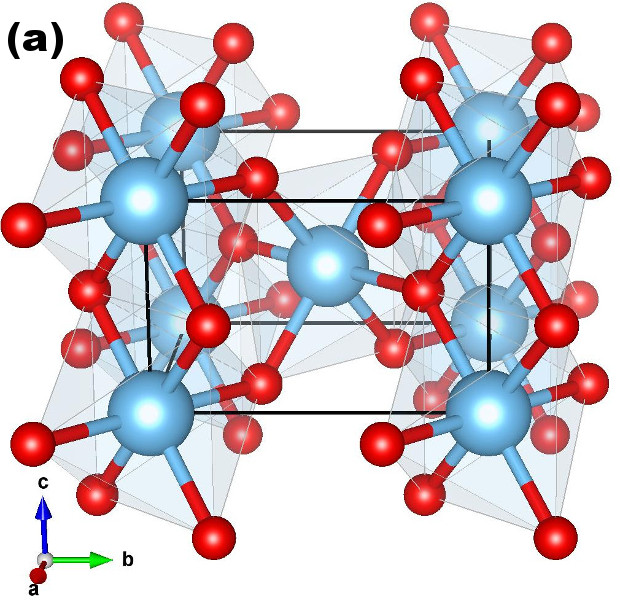
\includegraphics[height=5cm]{img/tio2-rutile.jpg}
  \qquad
  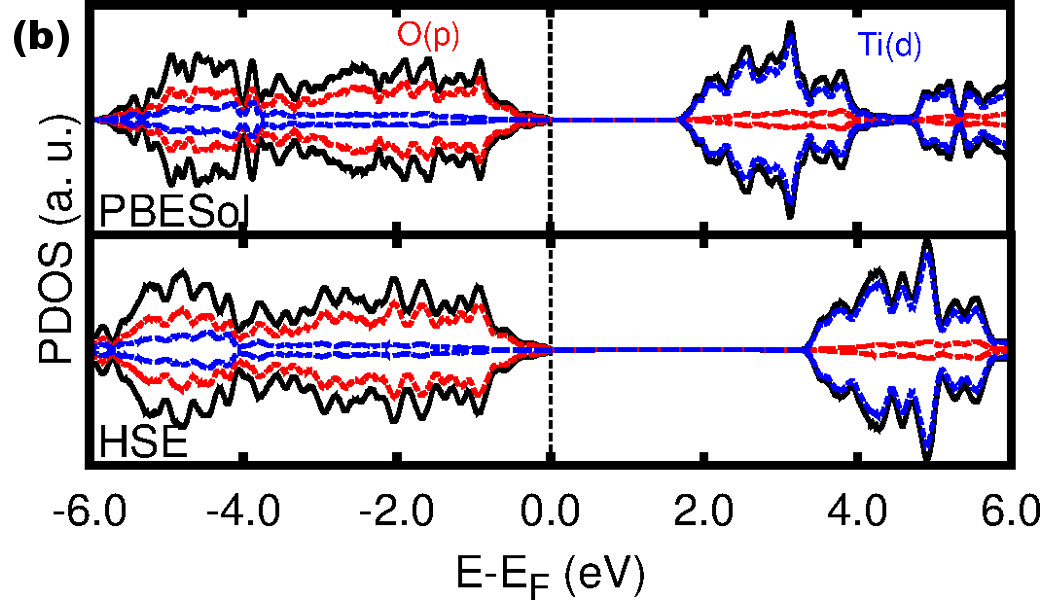
\includegraphics[height=5cm]{img/dos-tio2-rutile.jpg}
  \caption{(a) TiO$_2$-rutile structure. Blue spheres are Ti atoms and red spheres are O atoms. TiO$_6$ octahedra are featured by the transparent blue polyhedra enclosing the Ti atoms. (b) PDOS of TiO$_2$-rutile obtained either by PBESol (upper panel) and HSE (lower panel) functionals. The two spin components are depicted by positive and negative values along the vertical axis, and the vertical dashed line features the valence band maximum (VBM). The contribution from Ti(d) to CB and O(p) to VB are depicted by the blue and red dashed lines respectively while total DOS is given by the black full line.} 
  \label{fig:tio2}
\end{figure}

Its structure is depicted in figure \ref{fig:tio2} (a) where one can see the corner-sharing arrangement between its TiO$_6$ octahedra. The projected density of states (PDOS) was obtained for this compound using both the PBESol and HSE functionals and are presented in figure \ref{fig:tio2} (b). From these graphs one can notice that while the valence band (VB) is composed mainly by O(p) orbital contribution, the conduction band (CB) is mainly of Ti(d) character. It is also noticeable that HSE delivers a bandgap energy much closer to the experimental value than PBESol. This bandgap underestimation is a well known deficiency of GGA functionals \cite{Perdew2001}.

\section{Ti$_2$O$_3$-corundum}
\label{sec:ti2o3}

TiO presents a large range of non-stoichiometric compounds, and the most oxygen-deficient one before titanium monoxide (TiO) is the corundum structure Ti$_2$O$_3$. This compound presents a rhombohedral structure with space group $R\bar{3}c$ where its basic units, the TiO$_6$ octahedra, are displaced in face-sharing pairs, as shown in figure \ref{fig:struct-ti2o3}.
\begin{figure}[!ht]
 \centering
  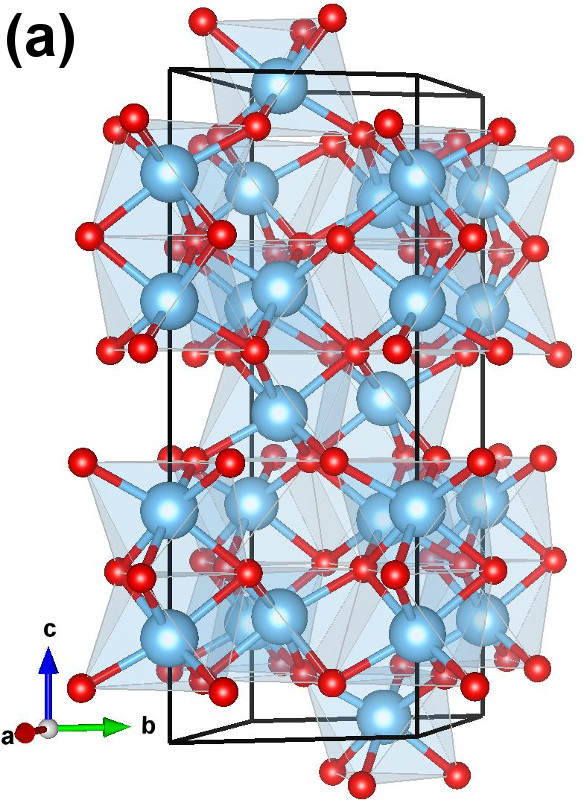
\includegraphics[height=7cm]{img/ti2o3-conv.jpg}
  \qquad
  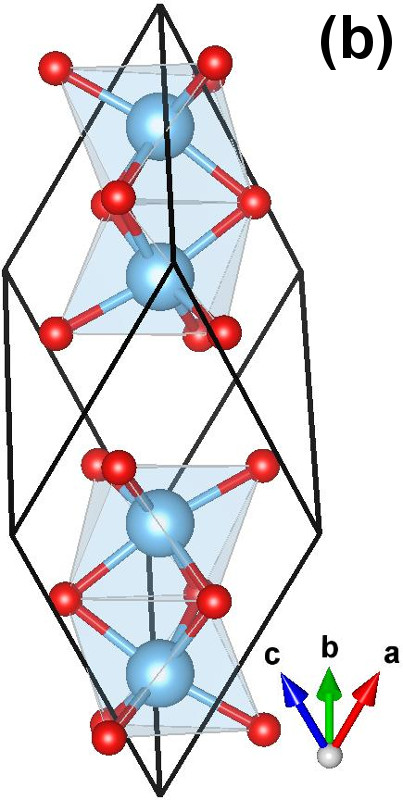
\includegraphics[height=7cm]{img/ti2o3-prim.jpg}
  \caption{Ti$_2$O$_3$ structures presented by the (a) conventional unit cell, and (b) primitive unit cell. Blue spheres are Ti atoms and red spheres are O atoms. TiO$_6$ octahedra are featured by the transparent blue polyhedra enclosing the Ti atoms.} 
  \label{fig:struct-ti2o3}
\end{figure}

As a first test of methodology, the band structure of the compound was obtained using the Local Density Approximation togheter with the Hubbard $U$ parameter (LDA$+U$), where the $U$ parameter was set to Ti(d) orbitals and its value was tuned in order to understand the impact in the final results. The same calculations were performed using the PBESol functional and the HSE functional for comparison. Results are presented in Figure \ref{fig:bands-ti2o3} where it is noticeable the effect of increasing $U$: two half-filled bands in $U = 0$ and PBESol calculations become splitted from the unoccupied bands above, thus revealing a semiconductor behavior for higher values of $U$ and for the hybrid HSE functional calculation\footnote{The $U$ parameter is usually employed in electronic structure calculations aiming to correct the DFT bandgap issue: the Local Density Approximation (LDA) and Generalized Gradient Approximation (GGA) are known to result in overestimated bandgaps. However, this bandgap correction is a consequence of a better localization of d or f electrons, due to an on-site Coulomb interaction (see appendix \ref{sec:app-dftu} and references therein for further details)}. This last result is in agreement with the experimental data, which states that this material is an insulator for low temperatures \cite{Uchida2008,Guo2012}.
\begin{figure}[!ht]
 \centering
  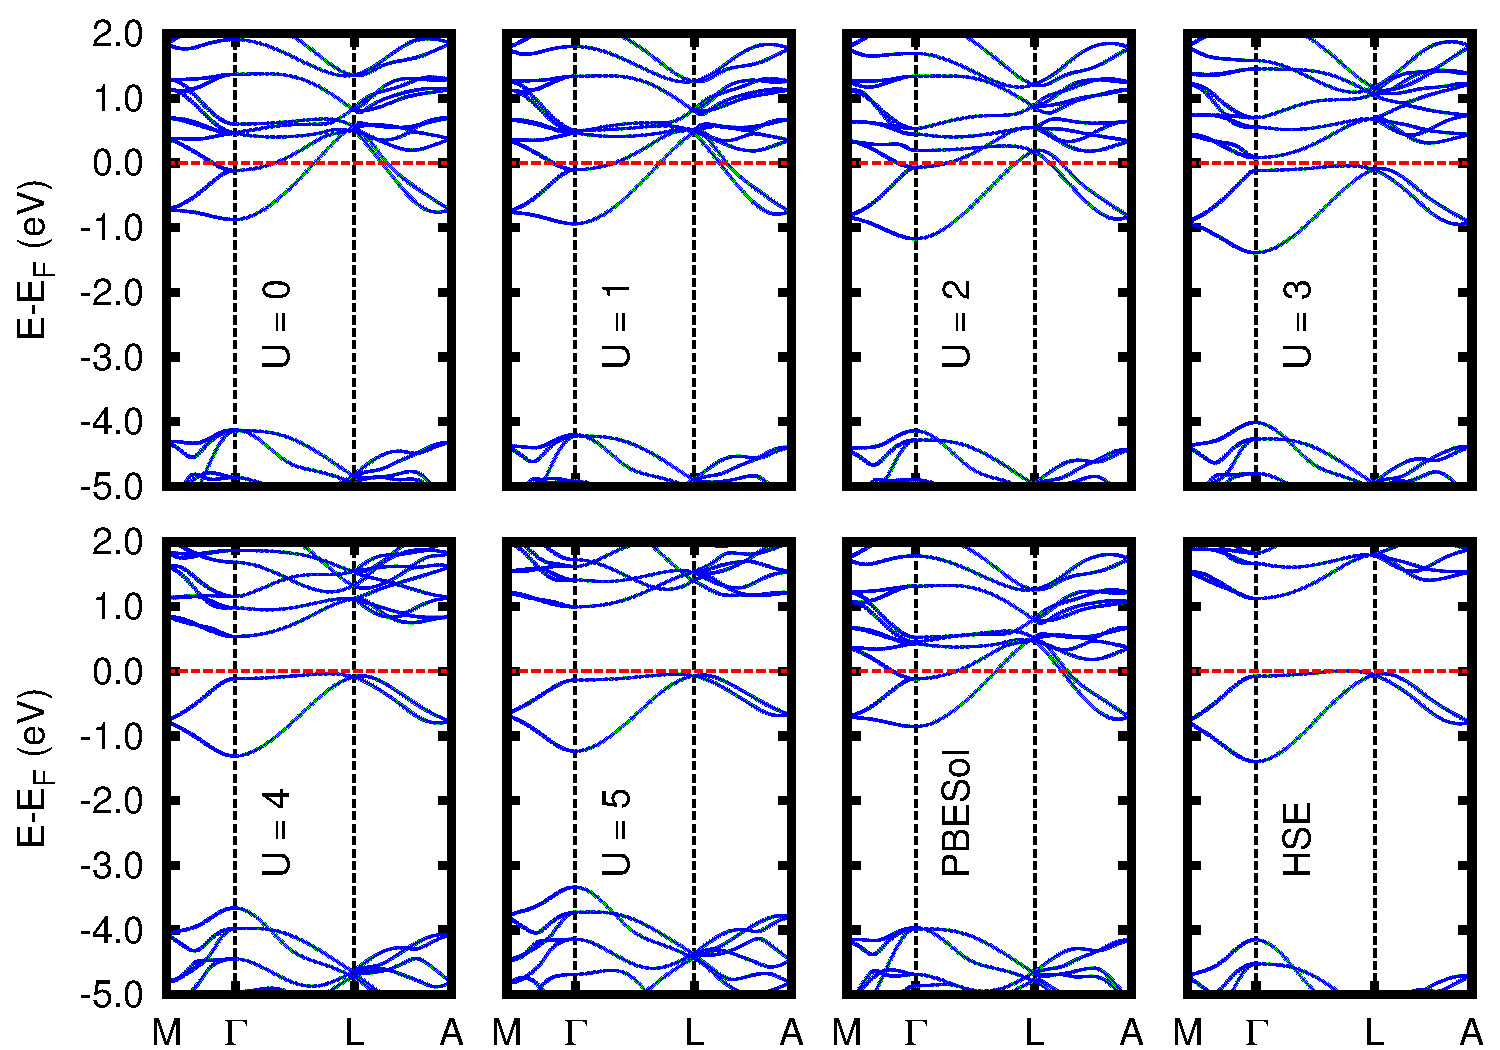
\includegraphics[width=0.95\textwidth]{img/ti2o3-bands.jpg}
  \caption{Band structure of Ti$_2$O$_3$ obtained using LDA+$U$ for increasing values of the Hubbard parameter $U$, ($0 \leq U \leq 5$) as well as PBESol and HSE functionals. The vertical red dashed line at zero energy is the Fermi energy. For $U \geq 3$ eV, as well as for the HSE calculation the system is a semiconductor, while in the other situations it is a metal.} 
  \label{fig:bands-ti2o3}
\end{figure}

 The PDOS was calculated using both PBESol, PBESol+$U$ ($U = 5$ eV) and HSE functionals and is presented in figure \ref{fig:dos-ti2o3-prb}. Once more the equivalence of the use of Hubbard $U$ and hybrid functional HSE is evident, and the incorrect description of a metal is provided solely by GGA functional PBESol. Another important information extracted form the PDOS is that the CB is mainly Ti(d), and when a bandgap is observed, the CB is also of the same character. In fact, this last occupied band can be regarded as an impurity band, very similar to the localized levels present in the TiO$_2$ bandgap when point defects are present \cite{Lee2012,Janotti2010}. The VB in this case can be identified as the levels laying around $-3$ eV for PBESol+U and $-4$ eV for HSE in figure \ref{fig:dos-ti2o3-prb}, mainly of O(p) character. In this picture, these systems have a large bandgap of $4-5$ eV and a filled intermediate band (IB) close to CBM, which could be an intrinsic $n$ dopant for the material.  
 
 \begin{center}
  \begin{figure}[ht!]
      \begin{center}
        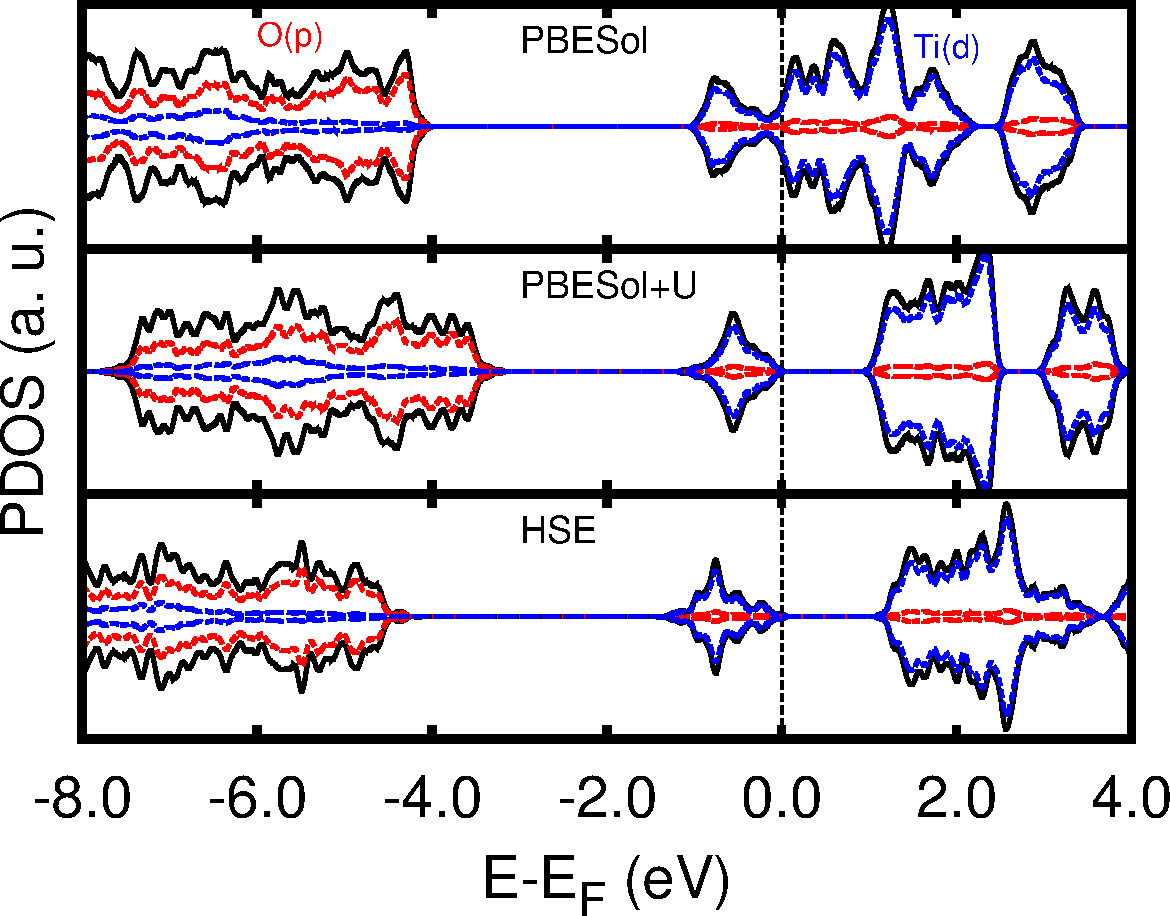
\includegraphics[width=0.6\textwidth]{img/dos-ti2o3-prb.jpg}
      \end{center}
      \caption{PDOS of Ti$_2$O$_3$ calculated by PBESol (upper panel), PBESol$+U$, where $U = 5$ eV (middle panel), and HSE (lower panel). The two spin components are depicted by positive and negative values along the vertical axis, and the vertical dashed line features the most energetic occupied level. The contribution from Ti(d) to CB and O(p) to VB are depicted by the blue and red dashed lines respectively while total DOS is given by the black full line.}.
      \label{fig:dos-ti2o3-prb} 
  \end{figure}
 \end{center}

The real-space projections of the IB (for PBESol the levels taken into account were the ones lower than $E_F$) are presented in figure \ref{fig:parchg-ti2o3-prb}. From these projections, it is evident that both the PBESol$+U$ and HSE calculations resulted in better descriptions of the Ti(d)-like levels, presenting the same hybridization. This was expected due to the fact that the introduction of the $U$ parameter leads to a stronger localization of these electrons arising from the on-site Coulomb interaction while the HSE functional introduces a part of the exact exchange, leading to a partial cancellation of the self-interaction problem of DFT \cite{Kim2009}. For a more detailed discussion please see appendices \ref{sec:app-dftu} and \ref{sec:app-hybrid}.
 \begin{center}
  \begin{figure}[ht!]
      \begin{center}
        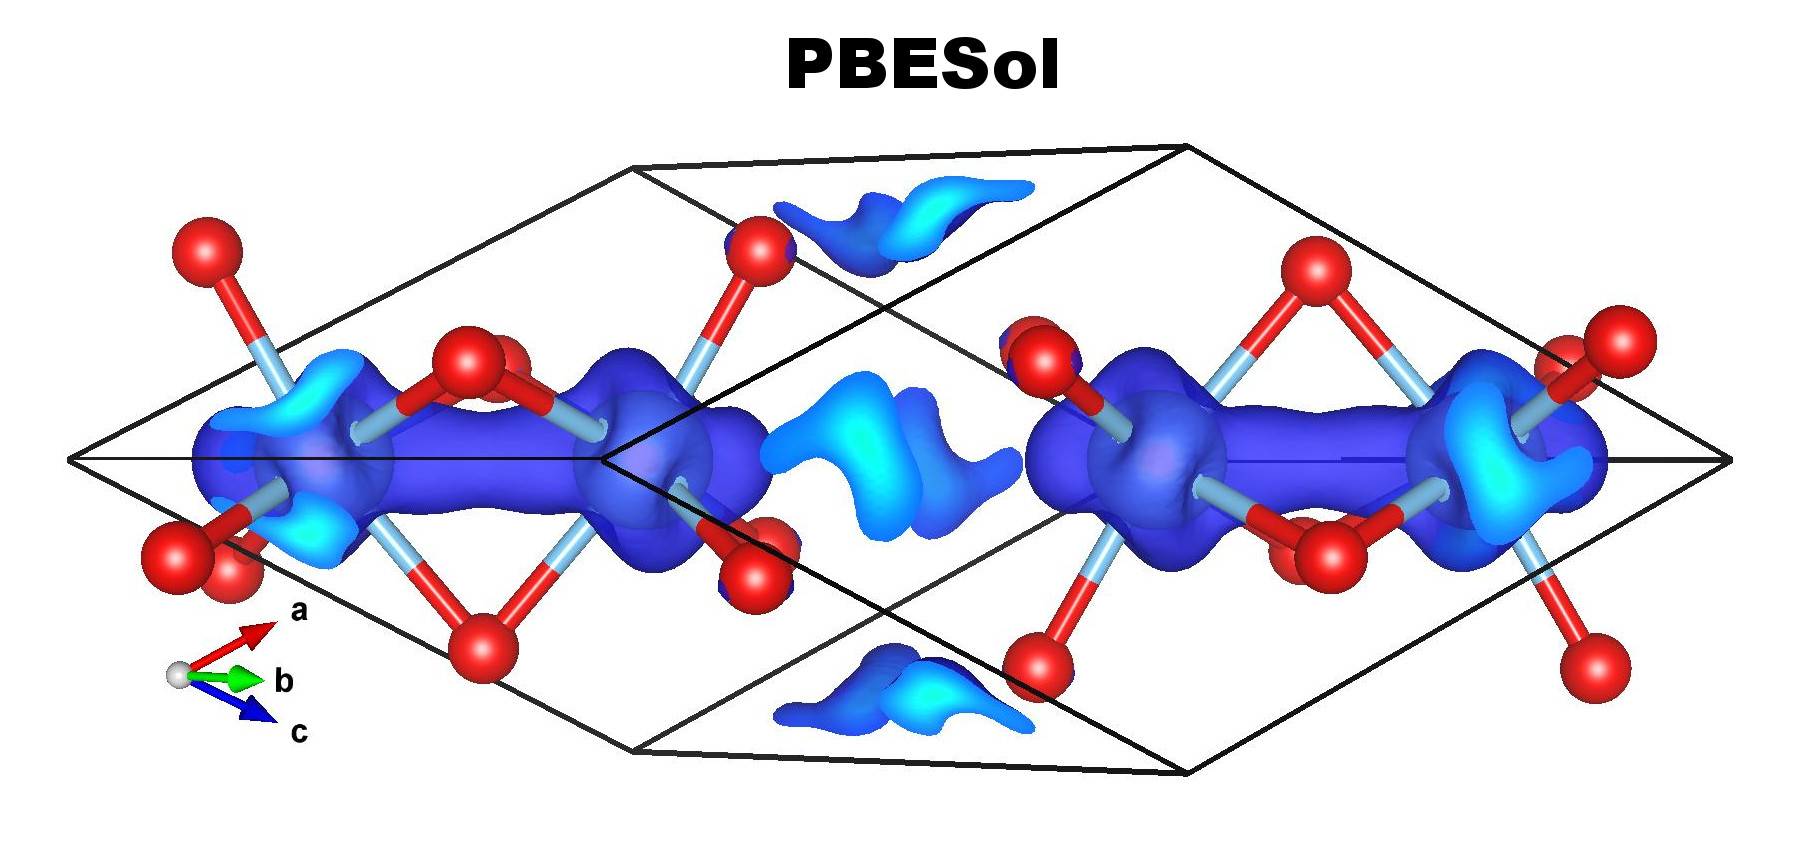
\includegraphics[width=0.3\textwidth]{img/ti2o3-parchg-pbesol+u-0.jpg}
        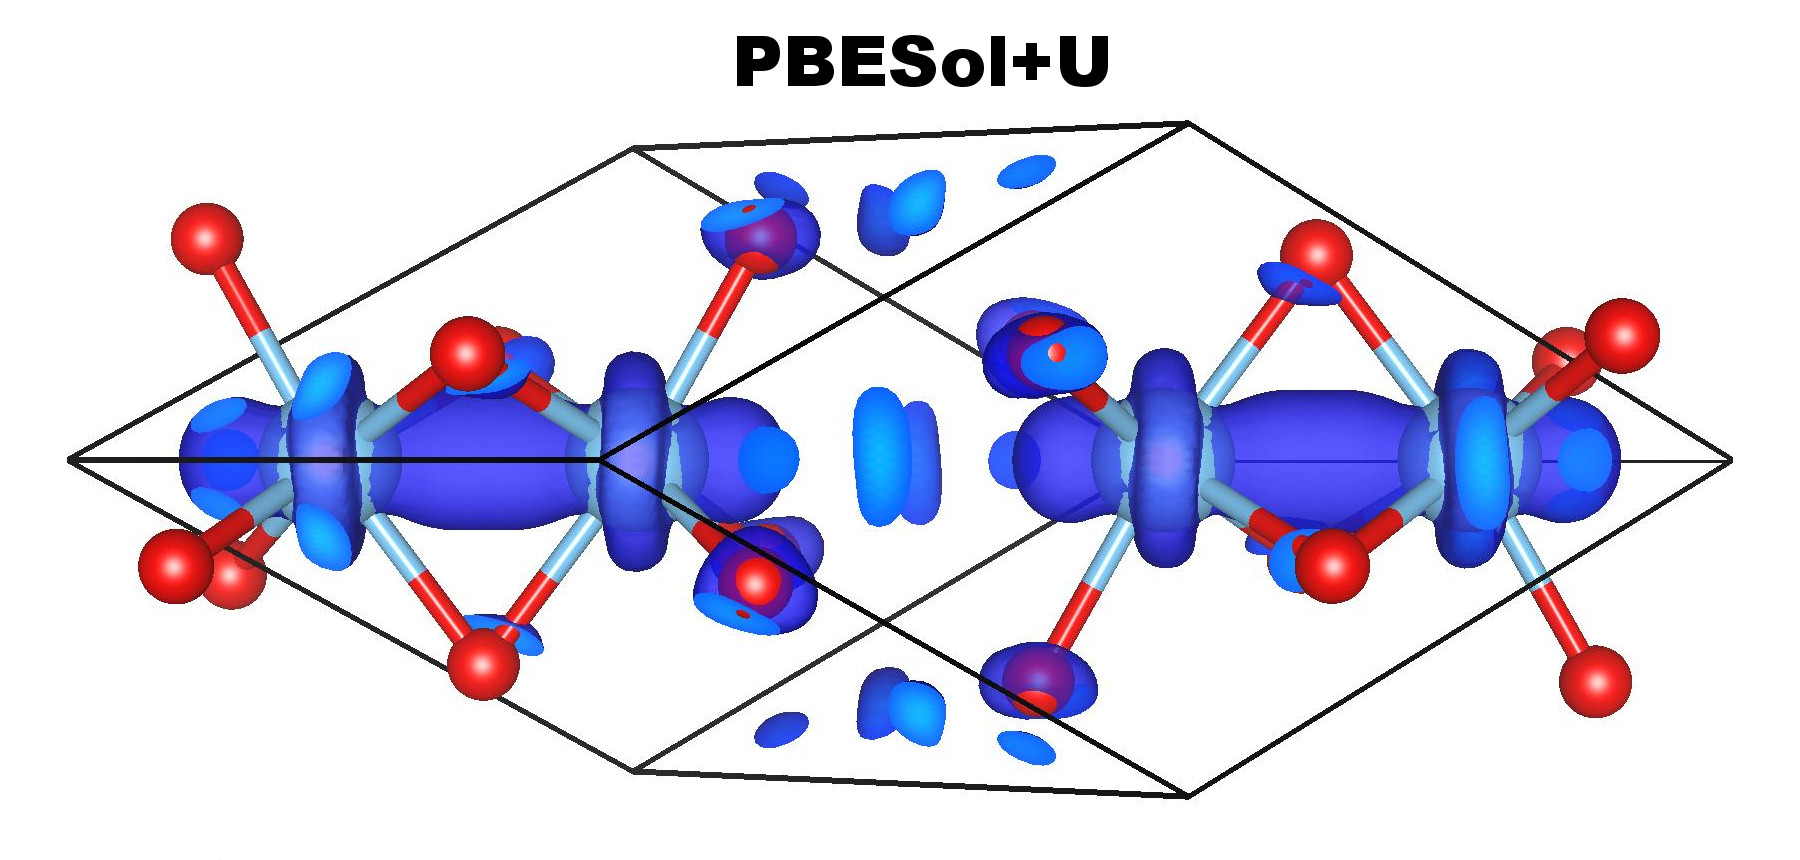
\includegraphics[width=0.3\textwidth]{img/ti2o3-parchg-pbesol+u-5.jpg}
        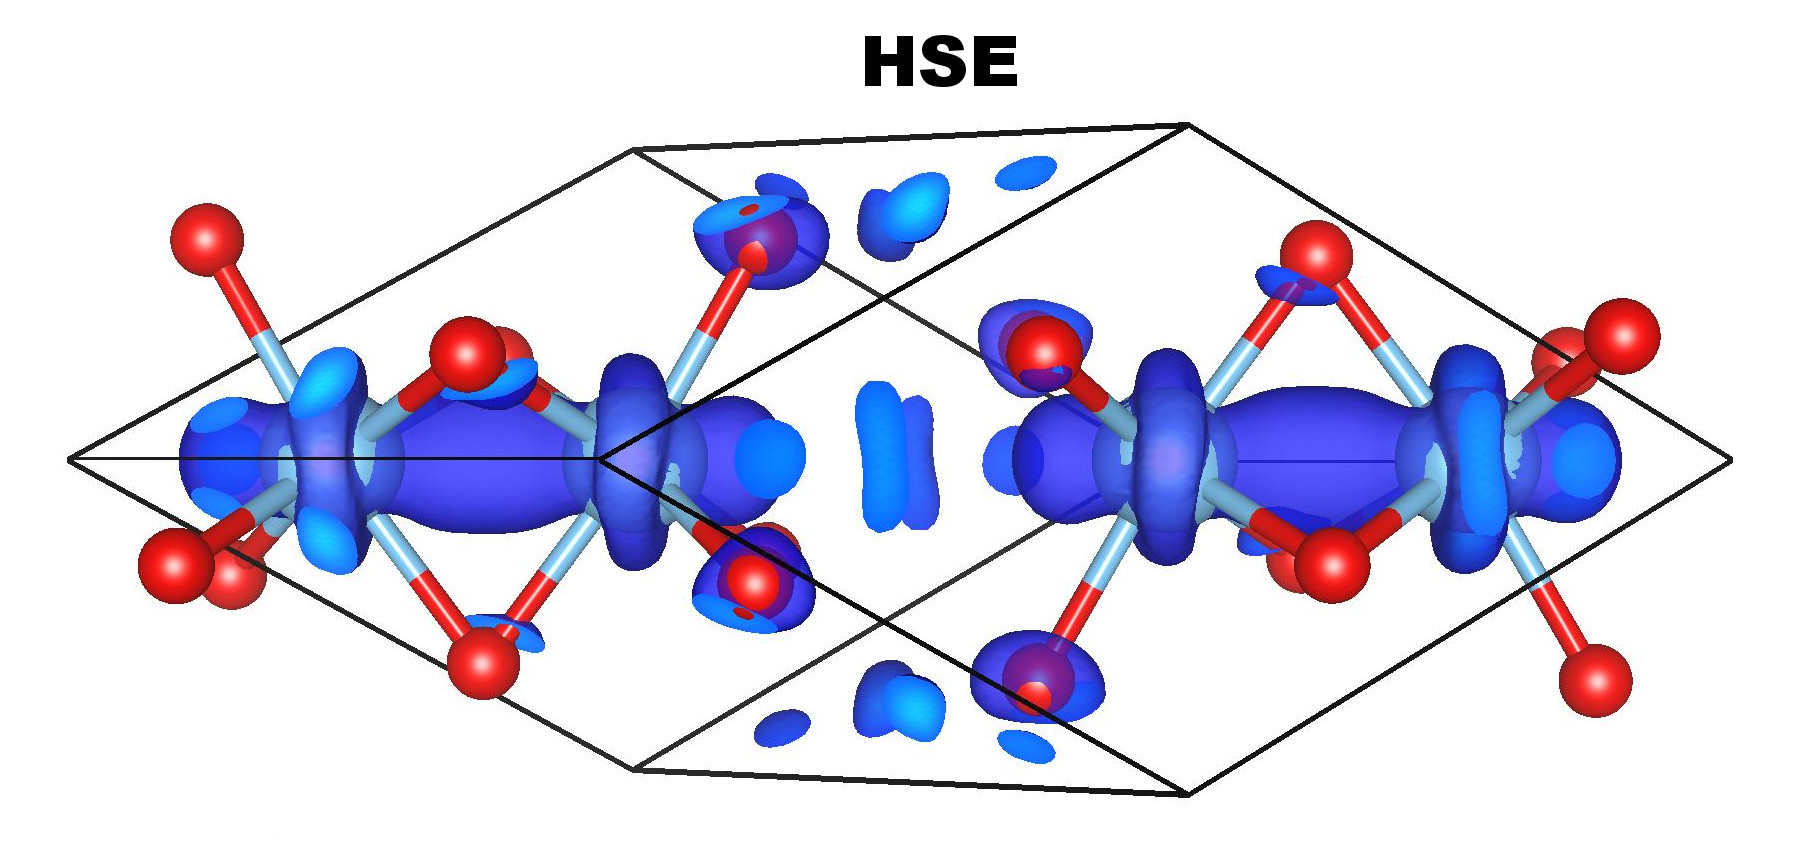
\includegraphics[width=0.3\textwidth]{img/ti2o3-parchg-hse.jpg} 
      \end{center}
      \caption{Real-space projection of the IB of Ti$_2$O$_3$ calculated by PBESol (left), PBESol$+U$, where $U = 5$ eV (middle), and HSE (right). The same isovalue of 1\% was used to plot the three bands.}.
      \label{fig:parchg-ti2o3-prb} 
  \end{figure}
\end{center}

\section{Ti$_3$O$_5$}

The crystal structure of Ti$_3$O$_5$ is not unique. A variety of phases were synthesized and characterized for this compound, thus, we chose to study the electronic structures of the three most common ones (presented in Figure \ref{fig:struct-ti3o5}): the $\alpha-$ (orthorhombic, anosovite-like, group $Cmcm$) \cite{Rusakov2002}, $\beta-$ (monoclinic, group C2/m) \cite{Asbrink1959,Grey1994}, and $\gamma-$Ti$_3$O$_5$ (monoclinic, $I2/c$) \cite{Hong1982}. A first-order phase transition at approximately $440-460$ K between $\alpha-$ and $\beta-$ phases was reported by Onoda \textit{et\ al.} \cite{Onoda1998} and another transition between $\beta-$ and $\gamma$-Ti$_3$O$_5$ close to $250$ K was reported by Hong and \AA sbrink \cite{Asbrink1959}. 
\begin{center}
  \begin{figure}[ht!]
      \begin{center}
        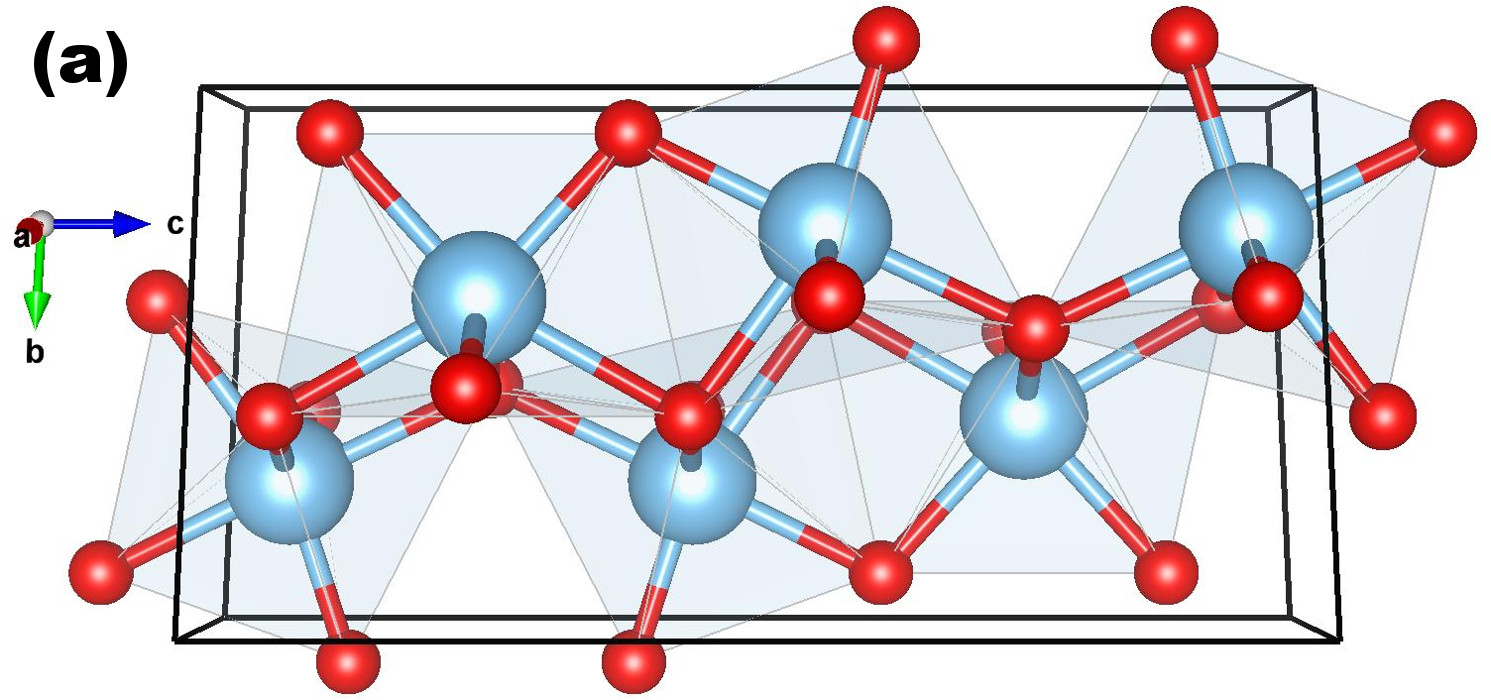
\includegraphics[height=2.5cm]{img/alpha-ti3o5.jpg}
        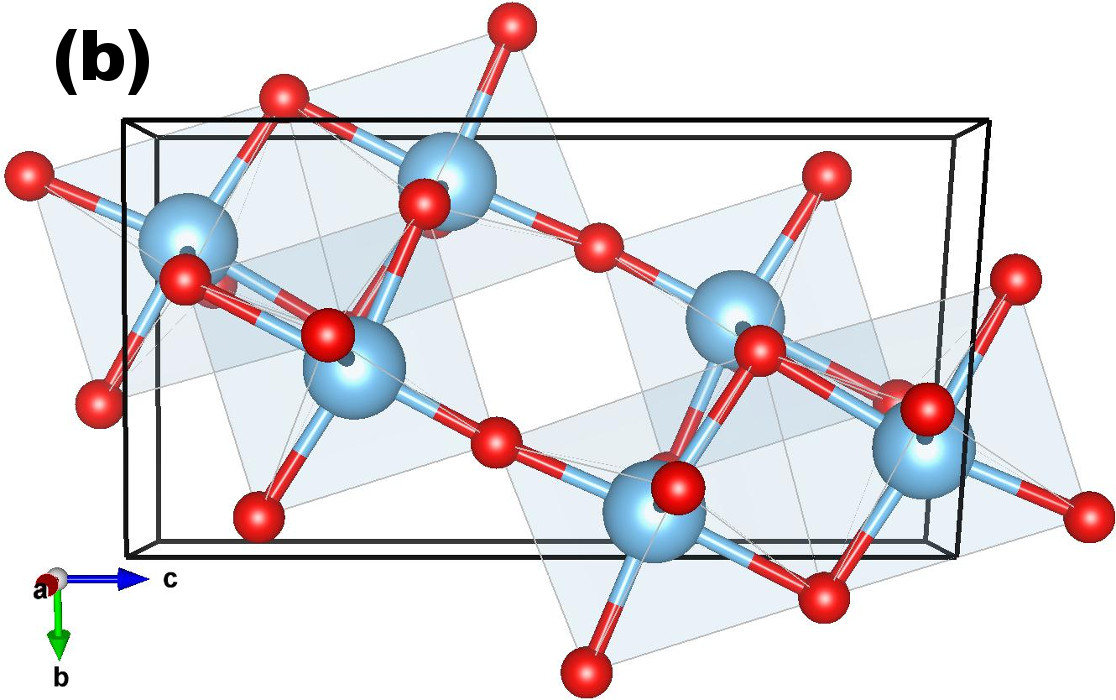
\includegraphics[height=2.5cm]{img/beta-ti3o5.jpg}
        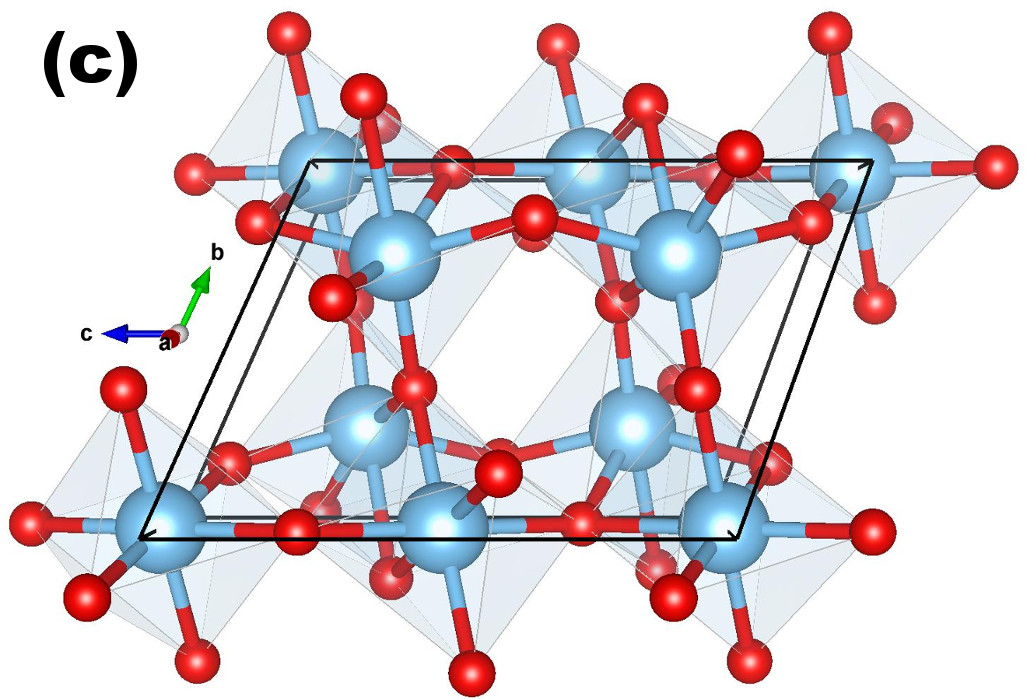
\includegraphics[height=2.5cm]{img/gamma-ti3o5.jpg} 
      \end{center}
      \caption{Crystalline structures of (a) $\alpha$-Ti$_3$O$_5$, (b) $\beta$-Ti$_3$O$_5$, and (c) $\gamma$-Ti$_3$O$_5$. Blue spheres are Ti atoms and red spheres O atoms. The TiO$_6$ octahedra are depicted in light blue.}
      \label{fig:struct-ti3o5} 
  \end{figure}
\end{center}

The PDOS for those three phases was obtained via the same methods employed for Ti$_2$O$_3$ and is presented in figure \ref{fig:dos-ti3o5-prb}. From these graphs, the same behavior as in the previous systems is noticed: the CB is mainly Ti(d), VB is mainly O(p), and IB's are basically of Ti(d) character and close to CBM. Also in this case the role of the functionals used for the calculations was evaluated, leading to the observation that the PBESol description as a metal is by no means correct---experimental data describe Ti$_3$O$_5$ as a semiconductor at low temperatures \cite{Rao1971,Bartholomew1969}. In fact, HSE calculations also resulted in metallic behavior for the $\beta$ and $\gamma$ phases, suggesting that this functional may not be the most suited for this system.
\begin{center}
  \begin{figure}[ht!]
      \begin{center}
        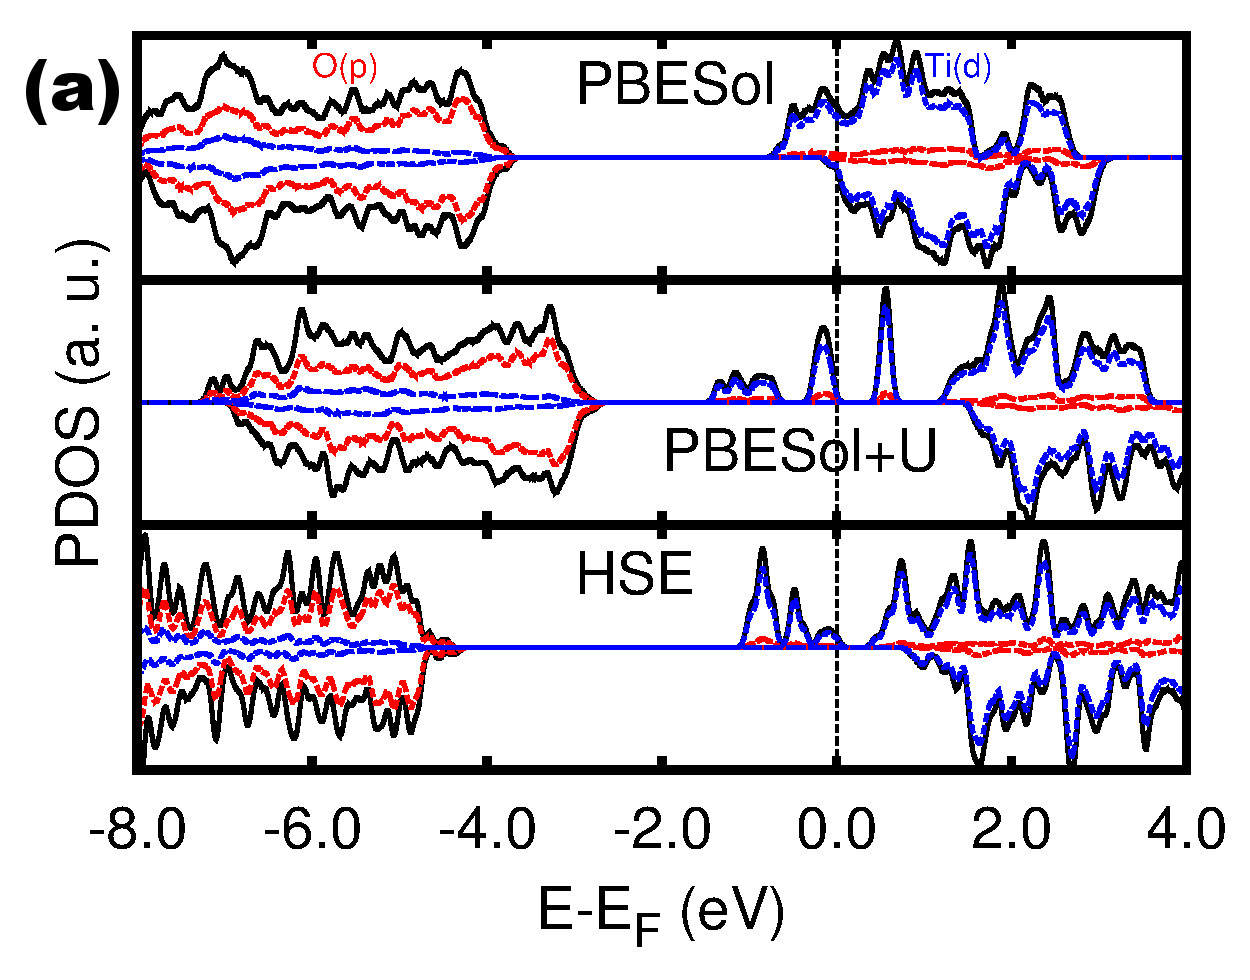
\includegraphics[width=0.3\textwidth]{img/dos-alpha-ti3o5.jpg}
        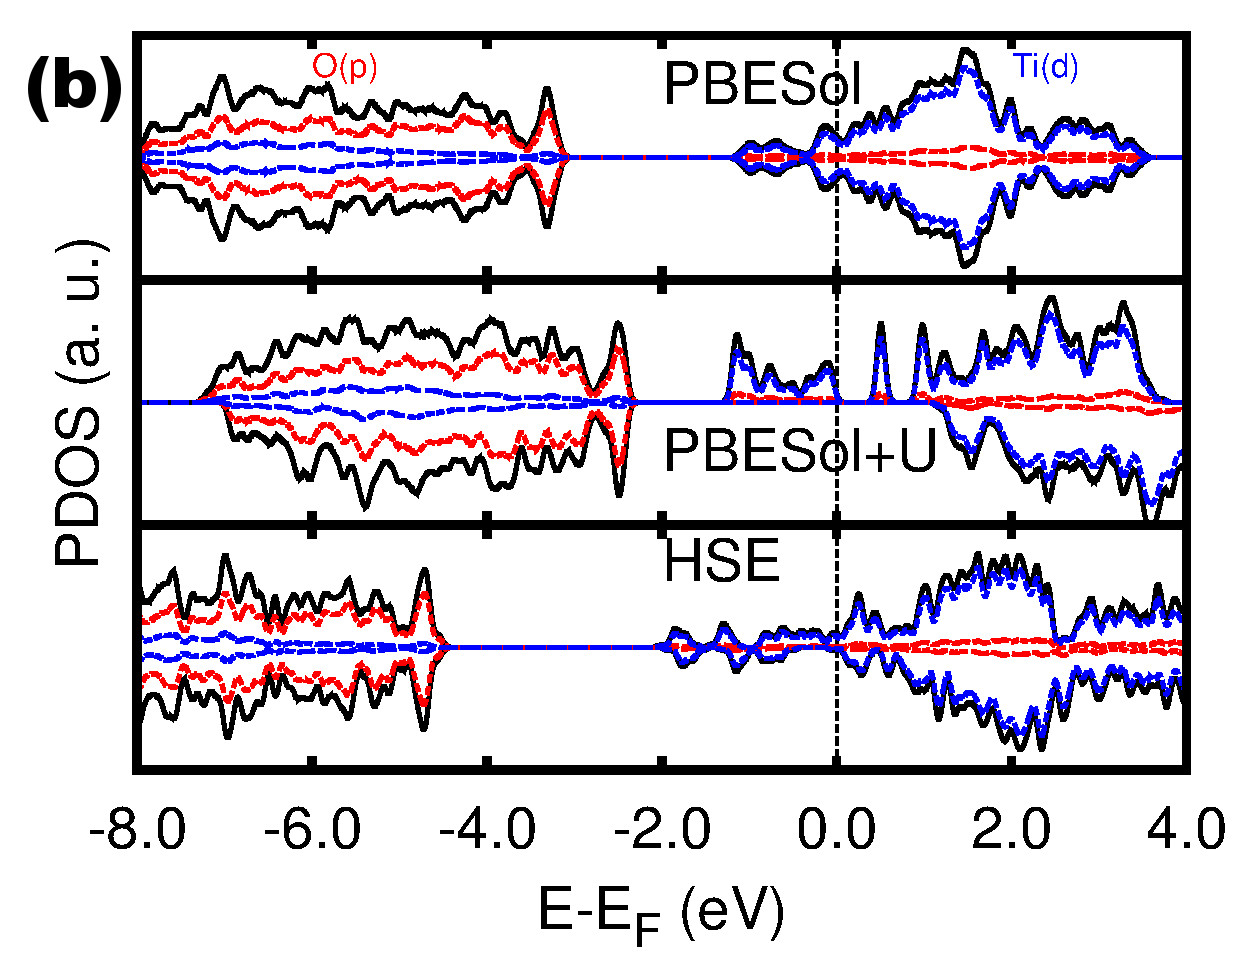
\includegraphics[width=0.3\textwidth]{img/dos-beta-ti3o5.jpg}
        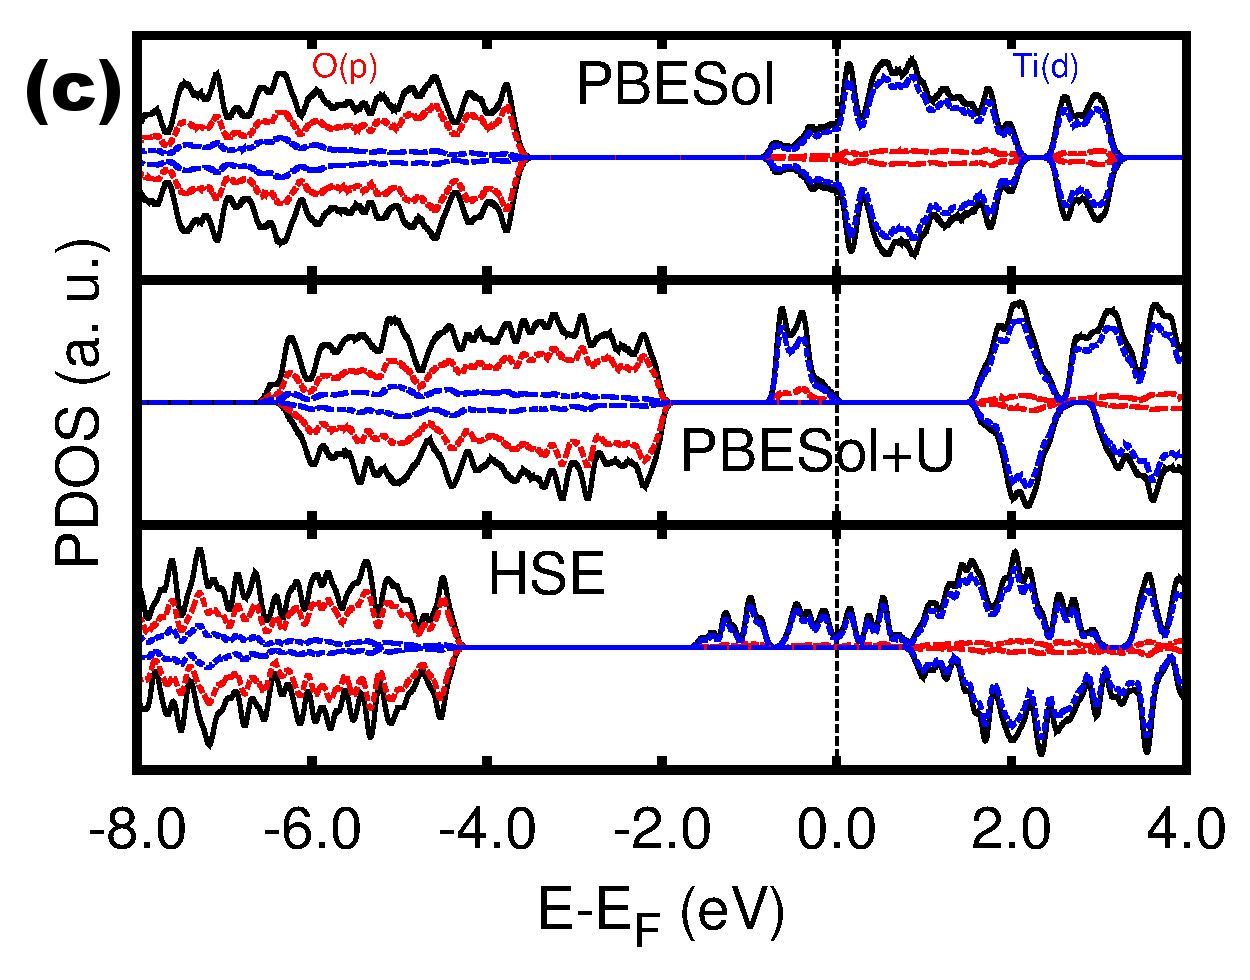
\includegraphics[width=0.3\textwidth]{img/dos-gamma-ti3o5.jpg} 
      \end{center}
      \caption{PDOS of (a) $\alpha$-Ti$_3$O$_5$, (b) $\beta$-Ti$_3$O$_5$, and (c) $\gamma$-Ti$_3$O$_5$ calculated by PBESol (upper panel), PBESol$+U$, where $U = 5$ eV (middle panel), and HSE (lower panel). The two spin components are depicted by positive and negative values along the vertical axis, and the vertical dashed line features the most energetic occupied level. The contribution from Ti(d) to CB and O(p) to VB are depicted by the blue and red dashed lines respectively while total DOS is given by the black full line.}.
      \label{fig:dos-ti3o5-prb} 
  \end{figure}
\end{center}

\section{Ti$_4$O$_7$ and Ti$_5$O$_9$ Magnéli phases}
\label{sec:magneli}

The results reported in this section, for both Ti$_4$O$_7$ and Ti$_5$O$_9$ Magnéli phases are the most important among those oxygen-deficient compounds, due to the fact that channels composed of these structures were detected inside memristors (see figure \ref{fig:canais-TiO}). 
\begin{figure}[!ht]
\centering
  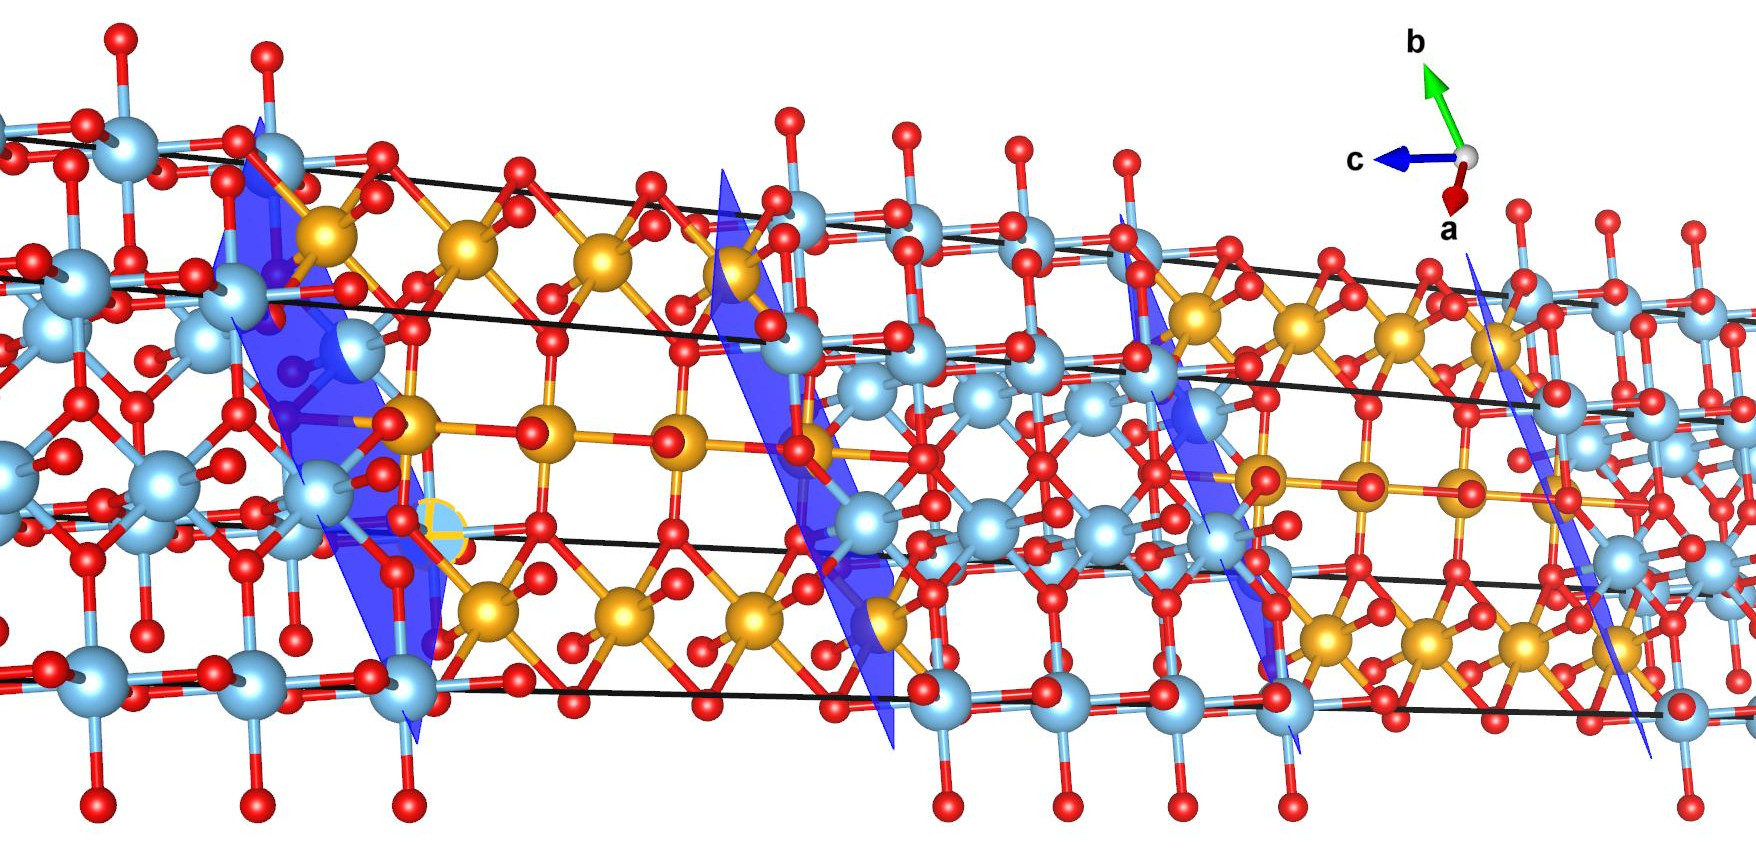
\includegraphics[width=0.9\textwidth]{img/ti4o7-multiple-c.jpg}
  \caption{Crystalline structure of Ti$_4$O$_7$. The blue and golden spheres are Ti atoms while the red spheres are O atoms. Different colors were used for Ti atoms to emphasize the rutile-like chains bounded by the shear planes, which are on the $ab$-plane and are featured in blue.}% The inset shows a cut of the same structure where the rutile-like chains are contained in the plane of the page. Ti$_5$O$_9$ presents a similar structure with one TiO$_6$ octahedra longer rutile-like chains.} 
  \label{fig:ti4o7-struct}
\end{figure}

All Magnéli phases are also composed of TiO$_6$ octahedra and present general formula Ti$_n$O$_{2n-1}$ ($4 \leq n \leq 10$), where $n$ is the number of octahedra in a rutile-like chain bounded by corundum-like structures. An illustration of the Ti$_4$O$_7$ structure is presented in figure \ref{fig:ti4o7-struct}. Ti$_4$O$_7$ presents three phases: low-temperature (LT, $T \leq$ 140 K), intermediate-temperature (IT, 140 K $\leq T \leq$ 150 K), and high temperature (HT, $T >$ 150 K) \cite{Bartholomew1969}. All phases present triclinic unit cell and space group $P\bar{1}$ \cite{LePage1984,Marezio1973,Marezio1971}, being the only difference between the structures a slight displacement of the atoms with respect to each other. After ionic relaxation, all structures converged to the same energy minimum with respect to ionic coordinates, thus, we report only the calculations for the LT phase. Ti$_5$O$_9$ has also a triclinic cell and space group $P1$ \cite{Andersson1960}.

The methodology employed for the previous materials was again tested for Ti$_4$O$_7$ calculations, and the band structure of this material is presented for LDA$+U$ functional [$0 \leq U \leq 5$ eV for Ti(d) electrons] in figure \ref{fig:bands-ti4o7}. The same behavior as in the Ti$_2$O$_3$ case was noticed: four bands became split from the unoccupied bands and a small gap of about 0.5 eV was observed when $U = 5$ eV.
\begin{figure}[!ht]
\centering
  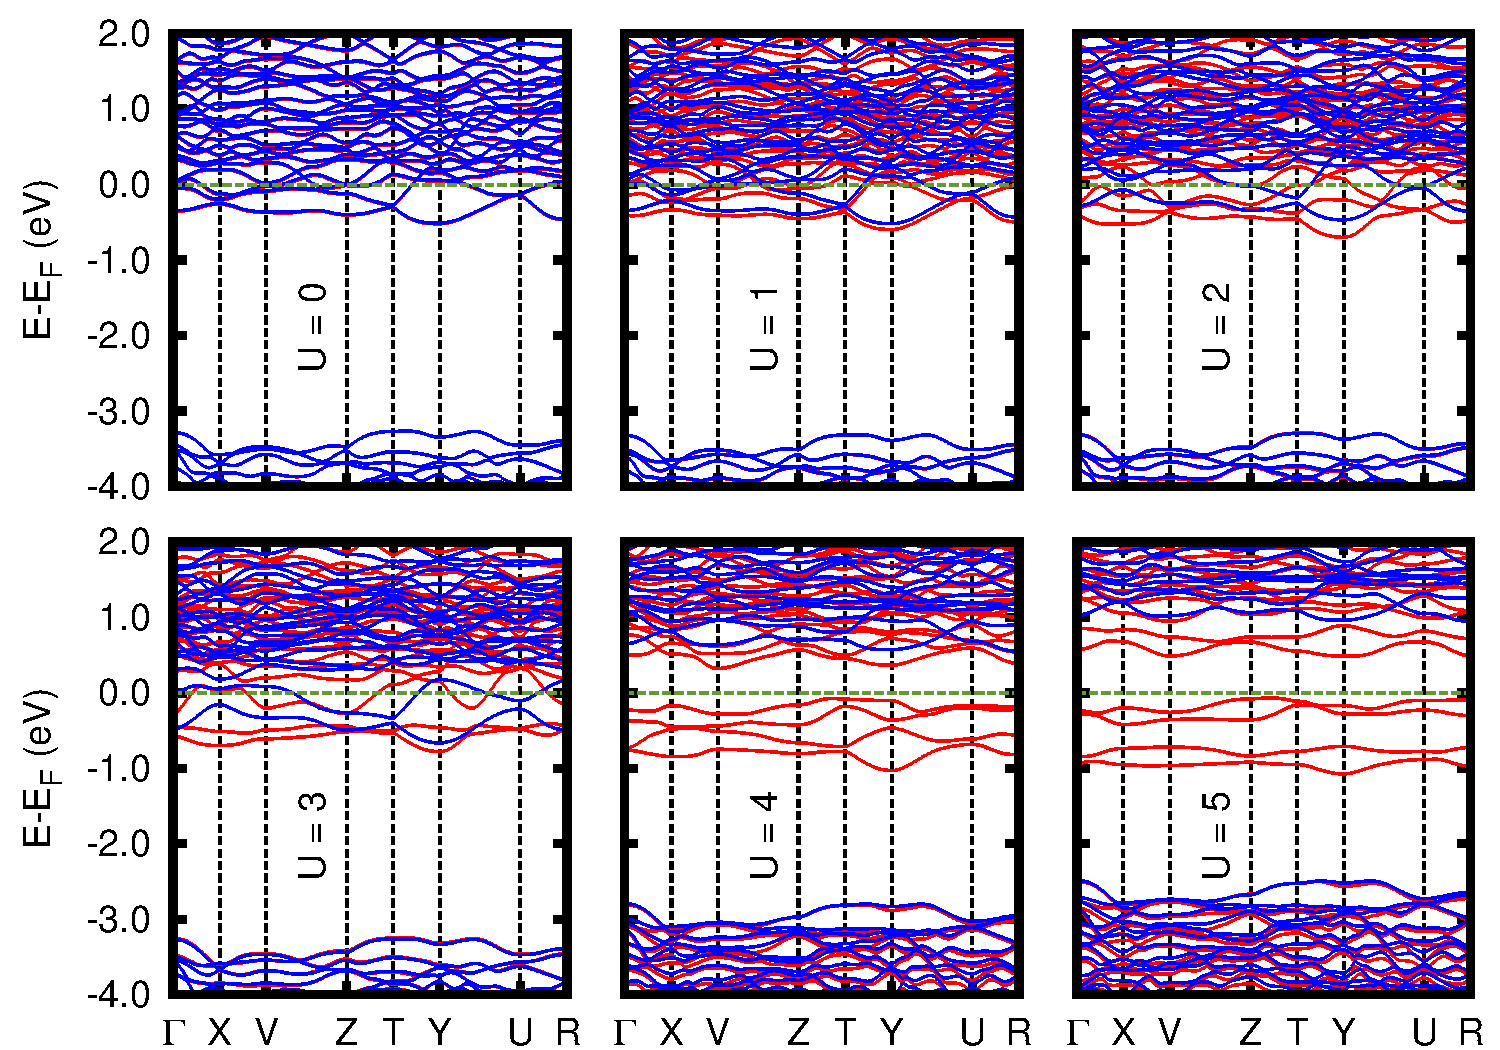
\includegraphics[width=0.95\textwidth]{img/bands-ti4o7.jpg}
  \caption{Band structure of Ti$_4$O$_7$ obtained using LDA+$U$ for increasing values of the Hubbard parameter $U$, ($0 \leq U \leq 5$). The spin components are plotted using either blue or red curves and the vertical green dashed line at zero energy is the Fermi energy. For $U = 4$ and $5$ the system is a semiconductor, while in the other cases it is a metal.} 
  \label{fig:bands-ti4o7}
\end{figure}

Comparison with PBESol, PBESol$+U$, and HSE functionals was made by plotting the PDOS of those systems. The results for both Ti$_4$O$_7$ and Ti$_5$O$_9$ are presented in figure \ref{fig:dos-magneli-prb}. From those graphs it is possible to notice that PBESol describes both systems as metals while the use of $U$ for Ti(d) electrons or HSE functional describe Ti$_4$O$_7$ and Ti$_5$O$_9$ as a small gap and large gap semiconductors respectively. The description of the electronic structure in these cases can be analogous to the previous discussion for Ti$_2$O$_3$: CB is mainly of Ti(d) contribution, VB is O(p), and IB has Ti(d) character. Comparison with experimental data in this case is difficult once there are no reports of the bandgap energy for Ti$_5$O$_9$, and for Ti$_4$O$_7$ a handful of values, from nearly metallic (0.041 eV from conductivity measurements \cite{Mulay1970}) to small-gap semiconductor (0.6 eV from spectroscopy analysis \cite{Abbate1995}), was reported.
\begin{center}
  \begin{figure}[ht!]
      \begin{center}
        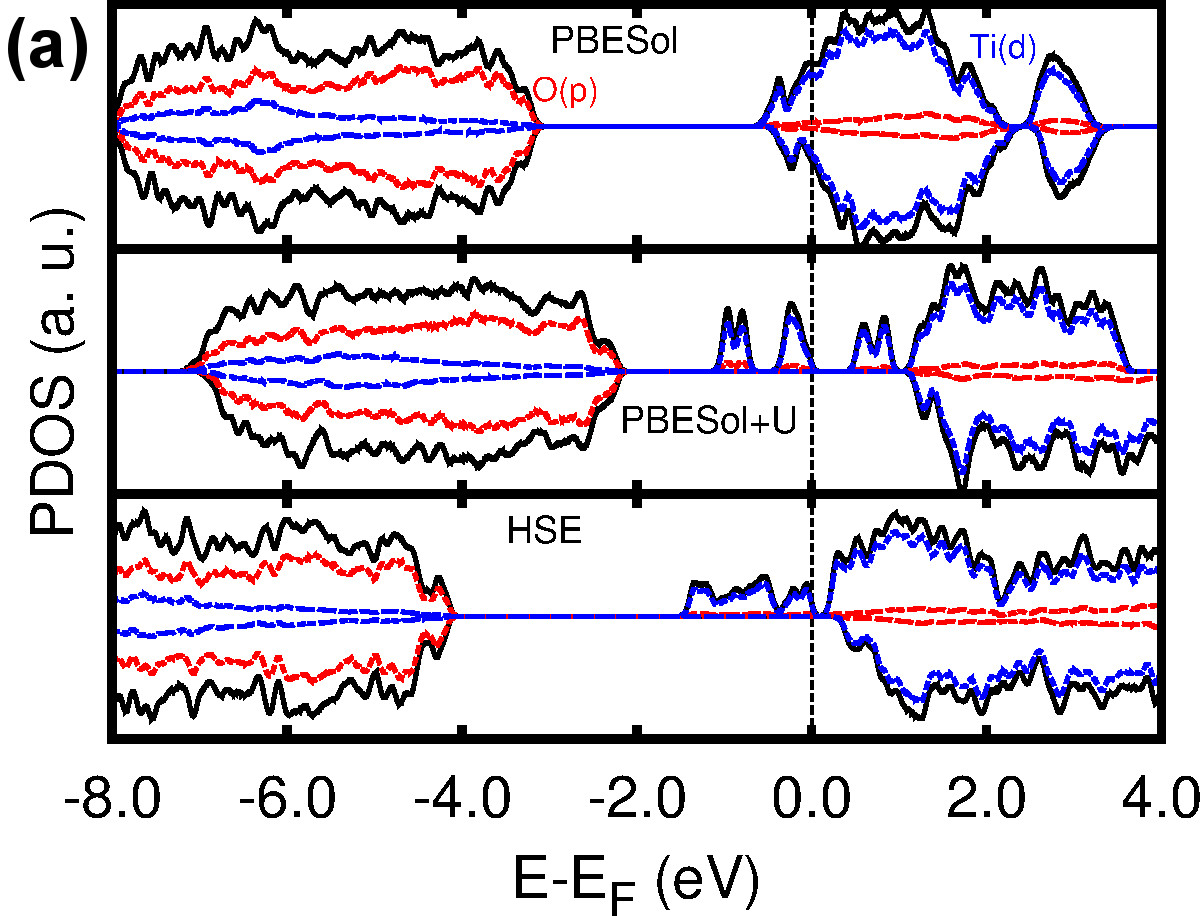
\includegraphics[width=0.45\textwidth]{img/dos-ti4o7-prb.jpg}
        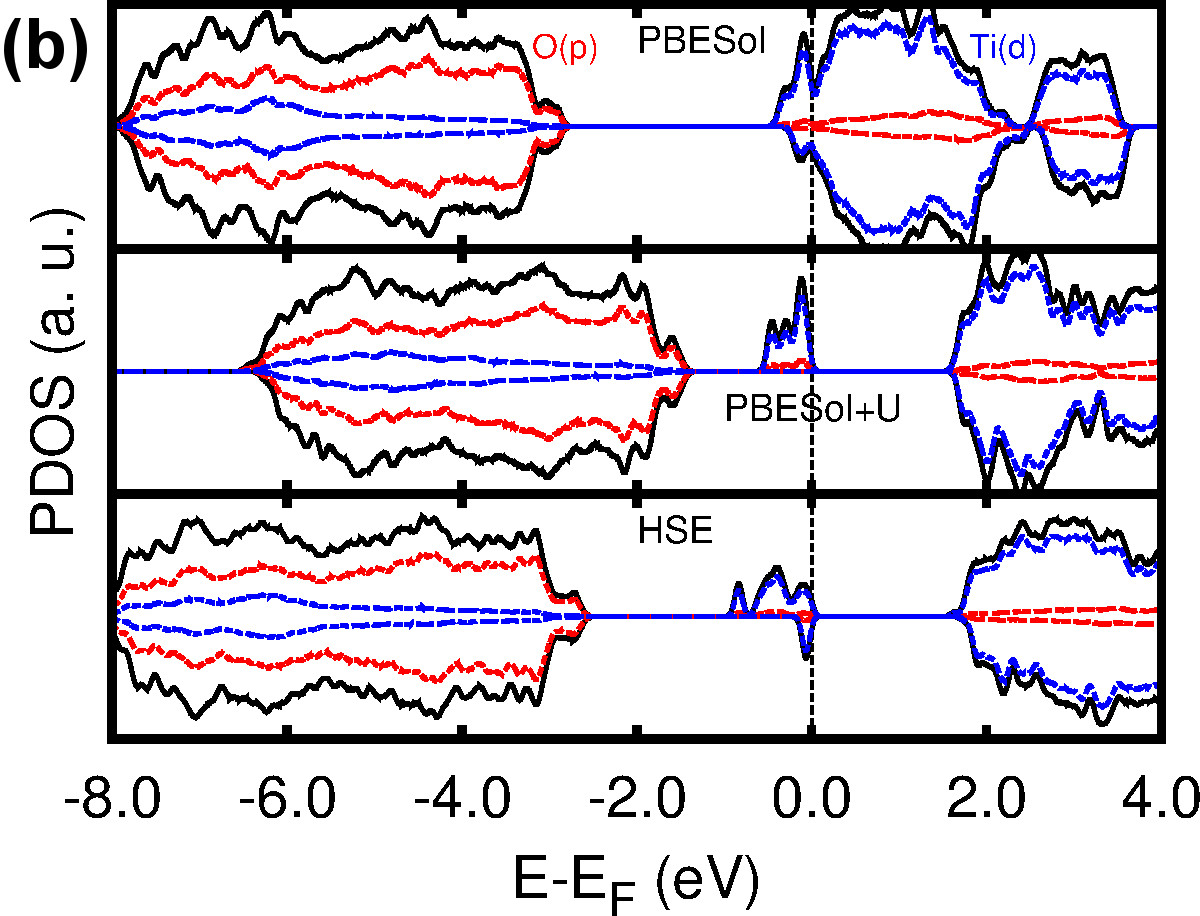
\includegraphics[width=0.45\textwidth]{img/dos-ti5o9-prb.jpg} 
      \end{center}
      \caption{PDOS of (a) Ti$_4$O$_7$, and (b) Ti$_5$O$_9$ calculated by PBESol (upper panel), PBESol$+U$, where $U = 5$ eV (middle panel), and HSE (lower panel). The two spin components are depicted by positive and negative values along the vertical axis, and the vertical dashed line features the most energetic occupied level. The contribution from Ti(d) to CB and O(p) to VB are depicted by the blue and red dashed lines respectively while total DOS is given by the black full line.}.
      \label{fig:dos-magneli-prb} 
  \end{figure}
\end{center}

Real-space projection of the IB of Ti$_4$O$_7$ was obtained in the same way as it was done for Ti$_2$O$_3$. The visual inspection of the orbitals plotted in figure \ref{fig:ti4o7-parchg} reveals a better localization by both PBESol$+U$ and HSE in comparison with PBESol calculation.
\begin{center}
  \begin{figure}[ht!]
      \begin{center}
        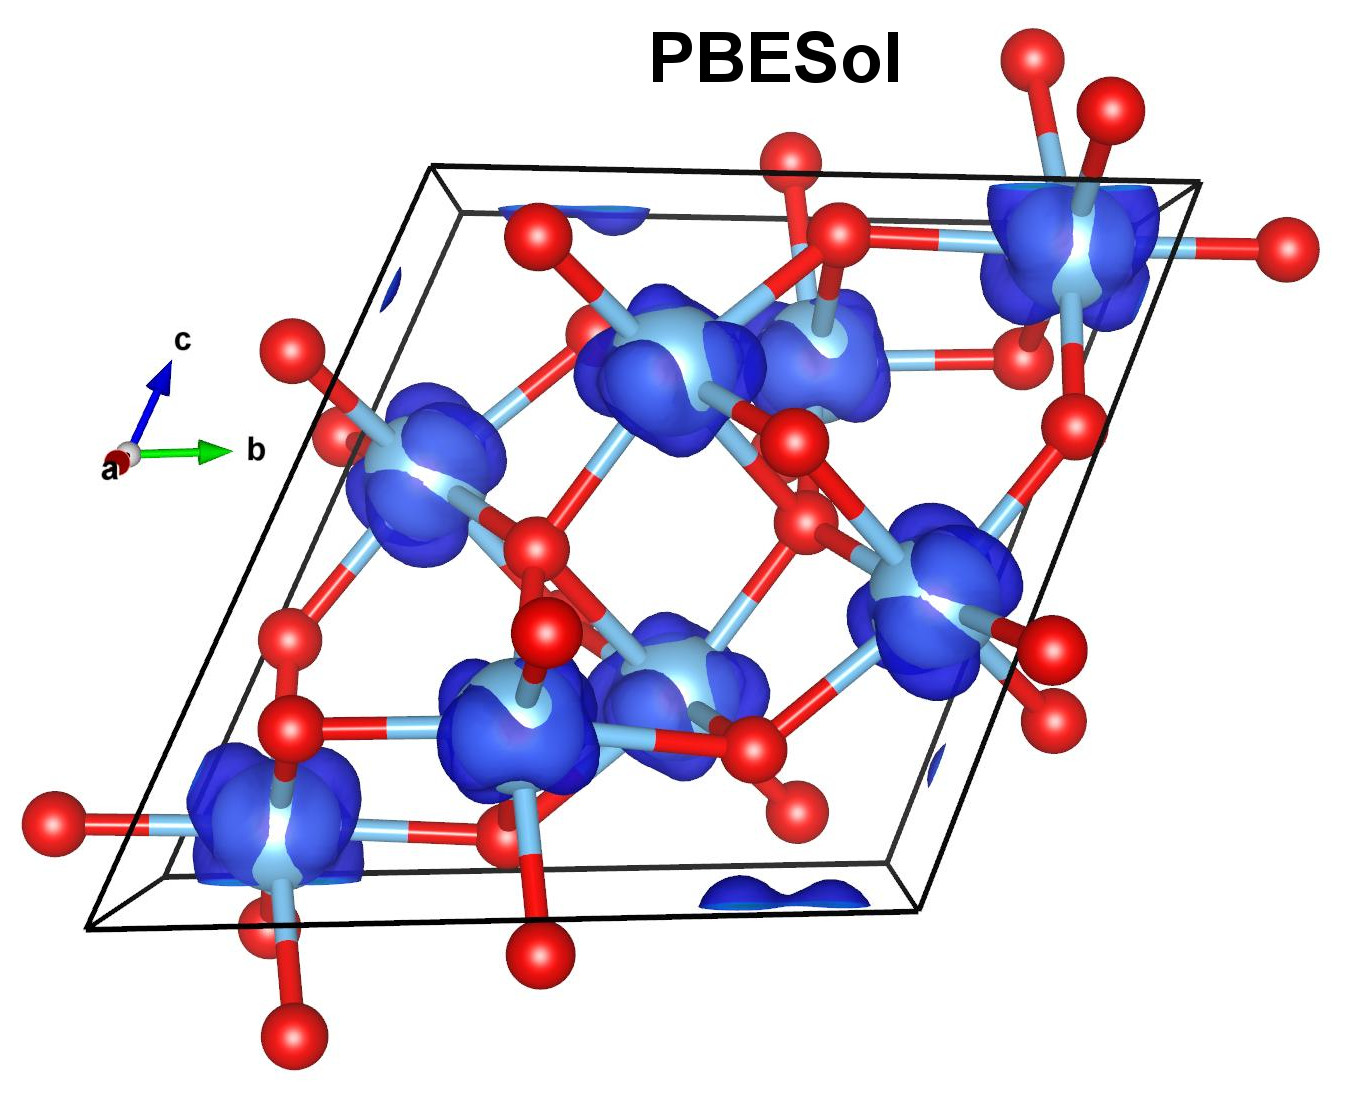
\includegraphics[width=0.3\textwidth]{img/ti4o7-parchg-pbsol+u0.jpg}
        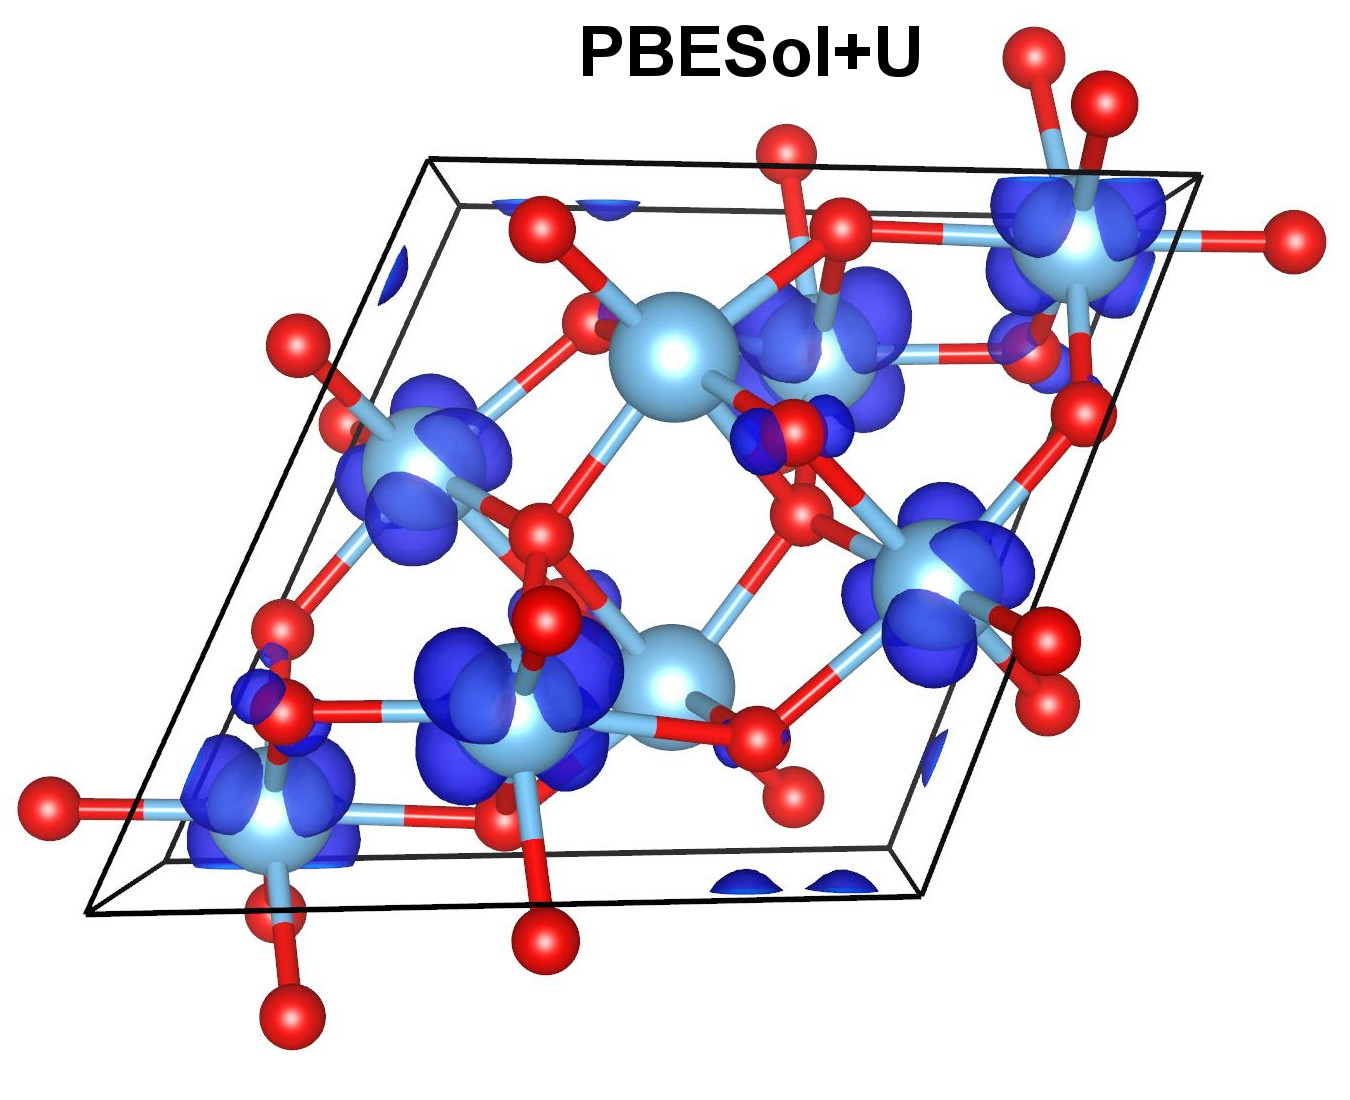
\includegraphics[width=0.3\textwidth]{img/ti4o7-parchg-pbsol+u5.jpg}
        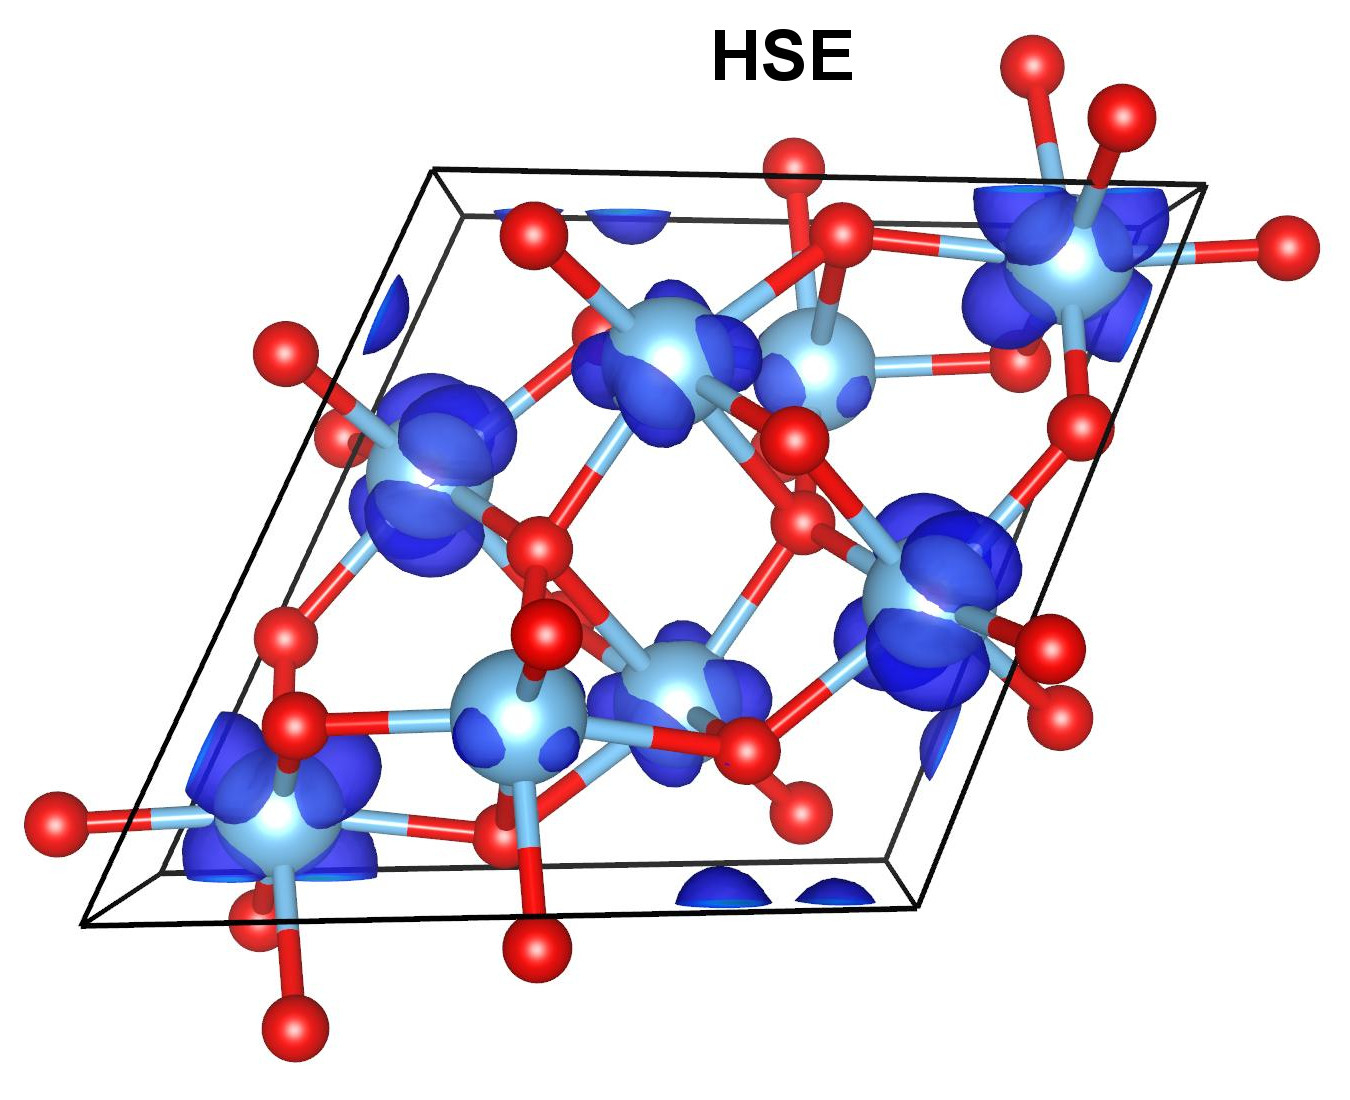
\includegraphics[width=0.3\textwidth]{img/ti4o7-parchg-hse.jpg}
      \end{center}
      \caption{Real-space projection over the primitive cell of the IB of Ti$_4$O$_7$ calculated by PBESol (left), PBESol$+U$, where $U = 5$ eV (middle), and HSE (right). The same isovalue of 1\% was used to plot the three bands.}.
      \label{fig:ti4o7-parchg} 
  \end{figure}
\end{center}

\section{Oxygen-deficiency in TiO$_2$}

Whenever native point defects are introduced into TiO$_2$, an excess of electron arises due to the deviation from stoichiometry. In the case of oxygen vacancy introduction (\textit{i. e.} the removal o oxygen atoms), a pair of unbound electrons is left behind, and if titanium interstitials are inserted, due to the $3d^24s^2$ configuration, a similar situation takes place \cite{Janotti2010,Lee2012}. With the exception of Ti$_2$O$_3$, which is a diamagnet at low temperatures \cite{Guo2012}, all the other oxygen-deficient phases of TiO$_2$ might present some degree of magnetism. Table \ref{tab:mags} shows the resulting total magnetization density per unit cell [$\mu(\mathrm{r})=\rho_{\uparrow}(\mathrm{r})-\rho_{\downarrow}(\mathrm{r})$] for all those systems. There it is noticeable that, with exception of $\beta$-Ti$_3$O$_5$ and Ti$_5$O$_9$, the magnetization density results for both PBESol$+U$ and HSE are essentially the same, indicating the presence of four parallel-spin electrons per cell\footnote{The unit cells of all systems presented here comprise two formula units, thus, the expected number in this case is indeed 4 $\mu_B$.}. This is an evidence of the better suitability of these methods rather than pure GGA functionals to study these crystals, and additionally, the PBESol$+U$ leads to even better results in comparison to HSE. This might be due to the fact that the energy landscape with respect to spin polarization degree of freedom presents a series of local minima, being necessary a more computationally expensive method to fully map the possible configurations of minimum energy, as \textit{e. g.} quantum dynamics or annealing methods.
\begin{table}[ht!]
  \centering
  \caption{\label{tab:mags} Total magnetization per unit cell in units of Bohr magnetons ($\mu_B$) for all Ti${}_n$O${}_{2n-1}$ structures presented in this work obtained with PBESol, PBESol$+U$, and HSE functionals.}
   \begin{tabular}{*{7}{c}}
  \hhline{=======} 
    & Ti${}_2$O${}_3$ & $\alpha$-Ti${}_3$O${}_5$ & $\beta$-Ti$_3$O$_5$ & $\gamma$-Ti$_3$O$_5$ & Ti${}_4$O${}_7$ & Ti${}_5$O${}_9$ \\
    \hline
   PBESol & -0.06  & 3.75   & 0.00    & 0.15    & 1.12       & 2.19                    \\
    %\hline
     PBESol$+U$ &  0.00    & 4.00   & 3.99     & 4.00   & 4.00       & 4.00           \\
    %\hline
  HSE &  0.00   & 4.00   & 0.94  & 4.00   & 4.00     & 2.75      \\ 
  \hhline{=======} 
   \end{tabular}
 \end{table}

As a final remark, these results point towards the existence of an \textit{intermediate band} inside the bandgap for all the oxygen-deficient phases of TiO$_2$. These levels are close to the conduction band in all cases, and their character is mainly of Ti(d). This is similar to what is reported about point defects in the TiO$_2$ \cite{Janotti2010,Lee2012}. Owing to the fact that the Fermi level lies above those levels, charge transfer from them to the unoccupied levels can take place if an external perturbation is introduced in the system, as an external voltage---this is exactly what happens in the operation of a memristor. 

Indeed, some of those systems were already studied by DFT calculations: Guo \textit{et al.} used a screened exact exchange functional and reported an indirect ($L-\Gamma$) bandgap of 0.55 eV for Ti$_2$O$_3$ in agreement with our calculations \cite{Guo2012}. The three phases of Ti$_4$O$_7$ were studied by Liborio \textit{et al.} using B3LYP hybrid functional, resulting in small gaps and electronic levels similar to our IB \cite{Liborio2009}, while Weissmann reported HT-Ti$_4$O$_7$ as a metal and both IT- and LT-Ti$_4$O$_7$ as semiconductors using LDA+$U$ level of theory \cite{Weissmann2011}. Leonov reported a bandgap of 0.29 eV using the same methods \cite{Leonov2006}. Slipukhina and Le\v{z}ai\'{c} reported a very similar behavior to what is reported in this chapter with respect to increasing values of the $U$ parameter \cite{Slipukhina2014}. Our results present a systematic comparison between methodologies, by using both the GGA functional PBESol without and with the Hubbard $U$, and the hybrid functional HSE, showing that are compatible with these previous reports, as well as with the experimental data on the electrical properties of these systems. In this sense, our contribution in the study of these oxygen-deficient phases is a step further in the literature, by showing that these methods are suitable for further, more intrincate studies on these materials, being the use of the Hubbard $U$ a faster a reliable way in comparison with hybrids. The majority of the results presented in this chapter were published in Physical Review B \cite{Padilha2014}. The article is attached to this thesis in appendix \ref{sec:app-pub}.     %chap 2
\chapter{Band Offset}
\label{chap:band-offset}

The next step on the bottom-up approach of the memristors is the simulation of the interfaces between the raw materials. Microscopy analysis shows the formation of Ti$_4$O$_7$ and Ti$_5$O$_9$ channels spanning a great part of TiO$_2$-based memristors (see Figure \ref{fig:canais-TiO}), but so far no theoretical work aiming to describe the electronic structure of such interface was presented. It is known that bulk Ti$_4$O$_7$ and Ti$_5$O$_9$ are metals in high temperatures \cite{Bartholomew1969}, but in the nanometric scale it may not be the case. As shown in the last chapter, these oxygen-deficient phases might donate electrons from the IB to the host material of the memristor, changing its properties. The knowledge of the electronic properties of the interfaces is then paramount to further investigate the memristor. With that goal in mind, we build a supercell which contains the Ti$_4$O$_7$-TiO$_2$ interface and obtain the valence band-offset of this system, thus, a common reference for all electronic levels is available and the band alignment is understood. 

This offset is a key quantity for many applications, such as heterojunction solar cells, where incoming photons create electron-hole pairs which in turn are separated due to the band offset, giving rise to electrical current \cite{Liu2013}. Another example is the separation of charge carriers in photocatalysis using the TiO$_2$-rutile and -anatase mixed-phase, which was elucidated by this type of calculations \cite{Scanlon2013}. In both cases the excitation of the electron from the valence band (VB) to the conduction band (CB) of one material and the migration of this electron to the CB of the other material due to the fact that its CB is lower in energy is the desired process, thus, the knowledge of the band offset is paramount.

In periodic calculations such as the ones performed in this step, the energies are given with respect to an arbitrary reference \cite{Ihm1979,Blochl1994}. This is a problem when one tries to compare energy levels of different structures, as is the case of the study of interfaces. The standard procedure in this case is the calculation of the average electrostatic potential, which is performed for the isolated materials and for bulk-like regions of a supercell containing the interface, and then the levels are shifted accordingly.

All results in this chapter were obtained by means of DFT calculations. The parameters used in the simulations are presented in appendix \ref{sec:app-calc}.

\section{Construction of the Ti$_4$O$_7$-TiO$_2$ interface}
\label{sec:interface}

One of the key points in the process of building an interface between two distinct materials is to match two of the three unit cell vectors of each compound in the interfacial region. Usually the individual unit cells are multiplied along the interfacial vectors' directions in order to impose the lowest strain on each phase, such that the deviation from the bulk electronic structure away from the interface is minimum. For the materials considered here, this is a very difficult task, owing to the fact that TiO$_2$ and Ti$_4$O$_7$ present very different unit cells (see sections \ref{sec:tio2} and \ref{sec:magneli} respectively).

To overcome this difficulty, two operations are performed to derive the Ti$_4$O$_7$ Magnéli structure from the TiO$_2$-rutile. The first operation is to transform the TiO$_2$ tetragonal unit cell into the Ti$_4$O$_7$ triclinic cell \cite{Wood1981} (see table \ref{tab:struct-relax-prb}):
\begin{equation}
 \begin{array}{cccc}
 \left[ \begin{array}{c} a_M^{(n)} \\ b_M^{(n)} \\ c_M^{(n)} \end{array} \right] & = & \left[ \begin{array}{ccc} -1 & 0 & 1 \\ 1 & -1 & 1 \\ 0 & 0 & 2n-1 \end{array} \right] & \left[ \begin{array}{c} a_r \\ b_r \\ c_r \end{array} \right],
 \end{array}
 \label{eq:transf}
\end{equation}
where $a_M^{(n)}, b_M^{(n)}$ and $c_M^{(n)}$ are the cell vectors of the Magnéli structure of index $n$. This operation only affects the unit cell, the ions are not displaced, thus the crystal after the use of equation \ref{eq:transf} is still TiO$_2$-rutile. The second operation involves the displacement of the ions according to the formula \cite{Andersson1960,Harada2010,Anderson19671393}
\begin{equation}
  (121) \frac{1}{2}[0\bar{1}1],
  \label{eq:displ}
\end{equation}
where $(121)$ refers to a crystallographic plane of the rutile unit cell, and $[0\bar{1}1]$ is a vector of the same structure. This operation can be understood by successive displacements of ions. All atoms above a $(121)$ plane which was shifted $n$ times along the $c$ vector of the rutile structure [see figures \ref{fig:tio2} (a) and \ref{fig:ti4o7-struct}] are shifted by $\nicefrac{1}{2}[0\bar{1}1]$. This process is repeated until all the possible planes within the unit cell were considered. Since this operation affects only the atomic positions, the unit cell is preserved in this step.

The transformations presented above result in identical unit cells, thus, no strain is present at the interface. For our calculations, we use $n = 4$ in equation \ref{eq:transf} in order to derive the Ti$_4$O$_7$ unit cell as well as the same value of $n$ for the periodic displacements given by equation \ref{eq:displ}. Next, both cells are extended in the $c$ direction by periodic repetition, resulting in the structures presented in figure \ref{fig:struct-interface} (a) and (b). The last step was simply to join the structures at the plane secant to the $c$ axis, which resulted in the structure presented in figure \ref{fig:struct-interface} (c). The extension of the unit cells before performing this joining operation is justified by the necessity to create a bulk-like region for each compound inside the final supercell.
\begin{center}
 \begin{figure}[ht!]
   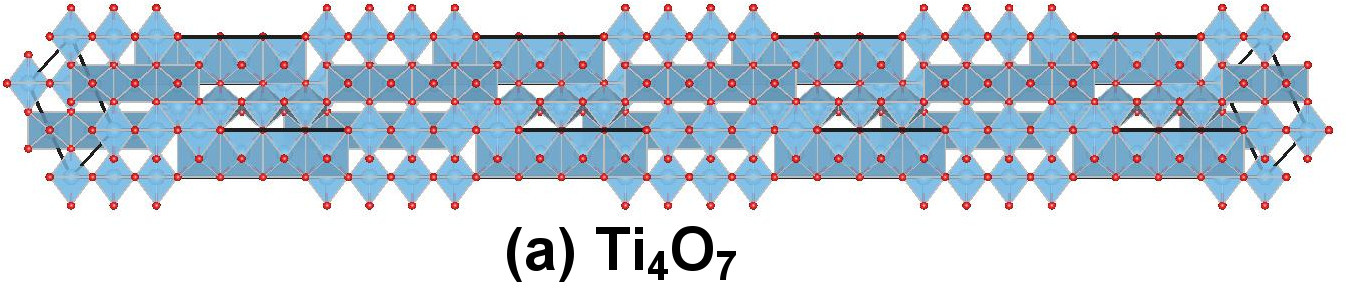
\includegraphics[width=0.5\textwidth]{img/ti4o7-big.jpg}
   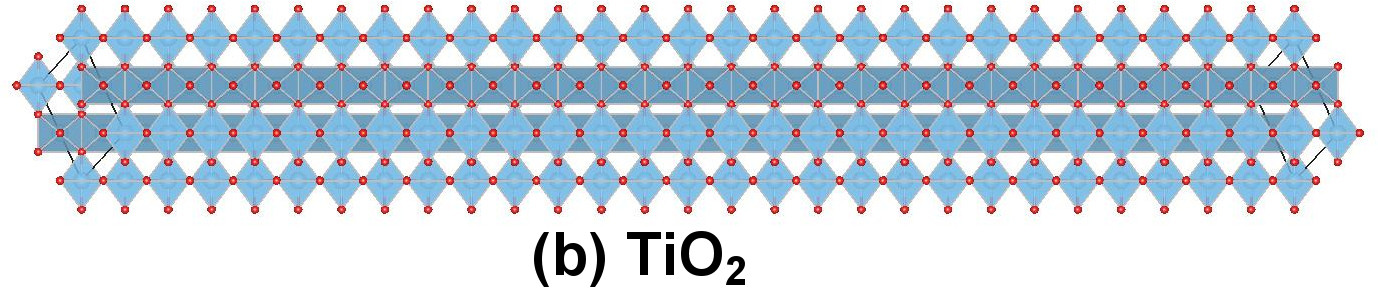
\includegraphics[width=0.5\textwidth]{img/tio2-big.jpg}
   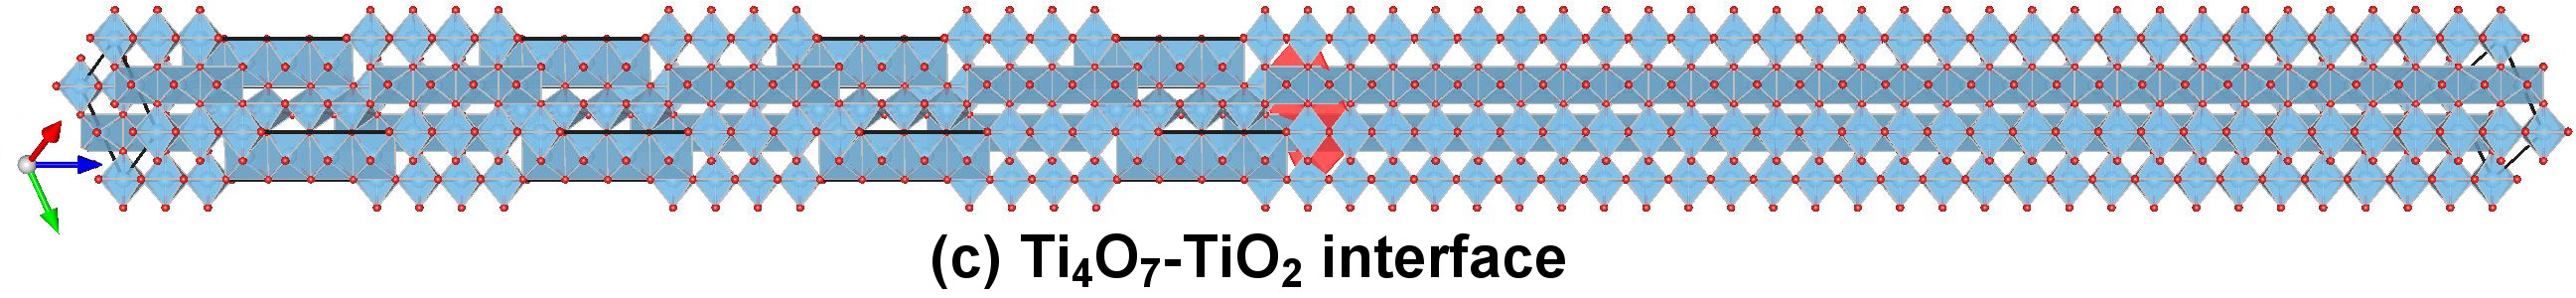
\includegraphics[width=1.0\textwidth]{img/interface-big.jpg}
  \caption{(a) Ti${}_4$O${}_7$ structure generated via the operations given by equations \ref{eq:transf} and \ref{eq:displ}, (b) TiO${}_2$ transformed according to equation \ref{eq:transf}, (c) and Ti${}_4$O${}_7$-TiO${}_2$ interface. The red plane in (c) indicates the interface region and the blue horizontal arrow corresponds to the $c$ crystal vector.}
  \label{fig:struct-interface}
 \end{figure}
\end{center}

\section{The band offset}
\label{sec:band-offset}

With the three structures obtained in the last section (both isolated materials and the supercell containing the interface), it is possible to calculate the valence band offset between the electronic levels of the bulk materials. The expression for the offset is given by \cite{Li2009b}
\begin{align}
 \Delta E_v(\text{TiO}_2|\text{Ti}_4\text{O}_7) =& \Delta E_{v,\phi}(\text{Ti}_4\text{O}_7)-\Delta E_{v,\phi}(\text{TiO}_2) \nonumber \\ &+\Delta E_{\phi}(\text{TiO}_2|\text{Ti}_4\text{O}_7),
 \label{eq:band-offset}
\end{align}
where $\Delta E_{v,\phi}(\text{Ti}_4\text{O}_7)$ and $\Delta E_{v,\phi}(\text{TiO}_2)$ are the differences between the Valence Band Maximum energy ($E_{VBM}$) and the electrostatic potential averaged over a certain volume of the unit cell of the isolated materials, while $\Delta E_{\phi}(\text{TiO}_2|\text{Ti}_4\text{O}_7)$ is the difference between the averaged electrostatic potential of the different materials calculated in bulk-like regions of the relaxed heterostructure supercell and the same averaged quantity obtained from the isolated material. An energy band diagram of the quantities involved in equation \ref{eq:band-offset} is presented in figure \ref{fig:bands-diagram}.
\begin{figure}[!ht]
\centering
  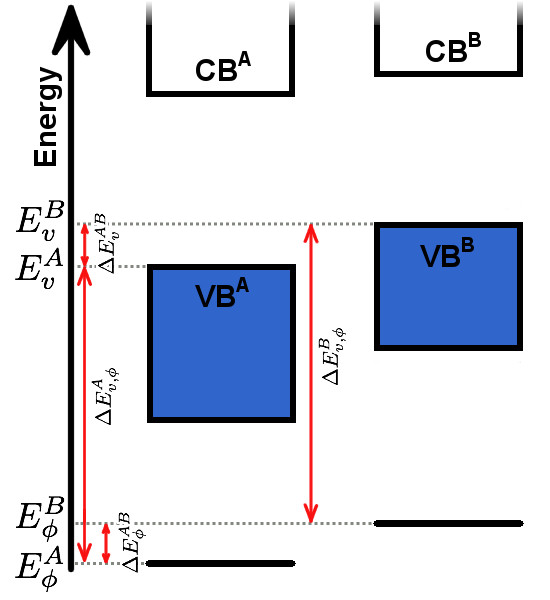
\includegraphics[width=0.5\textwidth]{img/band-offset-schematics.jpg}
  \caption{Band diagram of the valence band-offset between materials $A$ and $B$. $E_v^{A,B}$ and $E_{\phi}^{A,B}$ correspond to the energy of VBM and reference level of each material, respectively. $\Delta E_{v,\phi}^{A,B}$ is the energy difference between the reference energy level (in this work, the averaged electrostatic potential) and the VBM energy of compounds $A$ and $B$ respectively, while $\Delta E_{\phi}^{AB}$ and $\Delta E_v^{AB}$ are the offsets between the reference and the VBM's of the compounds.} 
  \label{fig:bands-diagram}
\end{figure}

Two of the quantities required by equation \ref{eq:band-offset} are readily obtained from DFT calculations using PBE$+U$ ($U = 5$ eV). This choice for the methodology is justified by the correct description of the oxygen-deficient phases presented in the previous chapter. In this manner, $E_{VBM}$ is obtained directly from the energy spectra of the isolated compounds, while the electrostatic potential [$\varphi(x,y,z)$] is obtained from the charge density calculated using the same method. The average of the potential along the $c$ axis is calculated by a simple integration along the planes secant to this vector,
\begin{equation}
 \phi(z) = \frac{1}{ab}\int_0^a \int_0^b \varphi(x,y,z) \, \mathrm{d}x \mathrm{d}y.
 \label{eq:partial}
\end{equation}
This average is plotted for all structures involved in the determination of the band offset in figure \ref{fig:potential}. In the potential profile it is possible to determine regions where the bulk potential is reproduced by the supercell results, being denoted by $\Delta z_1$ for the Ti$_4$O$_7$ part and $\Delta z_2$ for the TiO$_2$ part. The reference energy $E_{\phi}$ is obtained from the integration of $\phi(z)$ in those regions, either for the bulk materials as well as in the supercell. The values obtained from the bulk calculations for $E_{\phi}$ are used to calculate the first two terms of the right-hand side of equation \ref{eq:band-offset} while the ones obtained from the supercell are used in the last term.
\begin{center}
 \begin{figure}[ht!]
  \begin{center}
   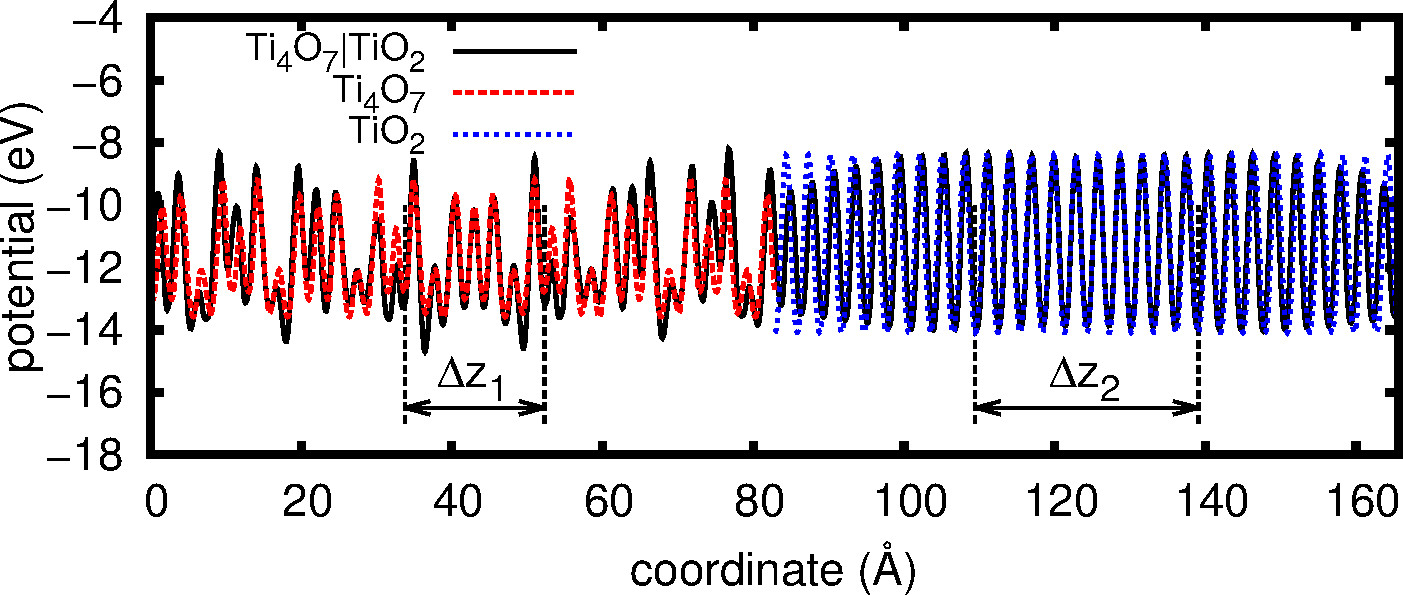
\includegraphics[width=0.9\columnwidth]{img/potential.jpg}
   \caption{Electrostatic potential profiles along the $c$ vector for all structures presented in this work: isolated TiO${}_2$ and Ti${}_4$O${}_7$, and the interface. $\Delta z_{1,2}$ denote the bulk-like region of the Ti$_4$O$_7$ and TiO$_2$ parts of the supercell, respectively.}
   \label{fig:potential} 
  \end{center}
 \end{figure}
\end{center}

The last step in this kind of calculation is the determination of the energy shift due to the strain introduced when interfacing the materials. Luckily in this case both cells used to build the interface are exactly the same by construction, thus, this final step presents no contribution. Finally, the calculated value for the valence band offset was $\Delta E_v (\text{TiO}_2|\text{Ti}_4\text{O}_7) = 2.18$ eV. The PDOS of both isolated systems is referenced by the TiO$_2$ VBM energy and the corresponding PDOS of Ti$_4$O$_7$ is shifted according to this result. These plots are presented in figure \ref{fig:pdos-bo}.

From the upper diagram in figure \ref{fig:pdos-bo} it is possible to extract two important informations: the localization of VBM and CBM in the compound system is at the Ti$_4$O$_7$ and TiO$_2$ respectively, and the energy difference between these levels---which is the bandgap---is 160 meV. However, by comparison with the results for the bulk Ti$_4$O$_7$ (section \ref{sec:magneli}) the last occupied level is the IB present in this structure, which can in turn donate electrons and $n$-dope the TiO$_2$. As the channels inside TiO$_2$-based memristors are made of Magnéli phases Ti$_4$O$_7$ and Ti$_5$O$_9$ channels immersed inside a TiO$_2$ matrix, this process of doping might take place inside the device, resulting in the change of the electronic properties of the active layer, and thus the electronic conductivity. This is further investigated in chapter \ref{chap:bandbend}, where the Poisson equation is solved for memristors and the role of the dopants in the transport properties is elucidated.

\begin{center}
 \begin{figure}[ht!]
  \begin{center}
   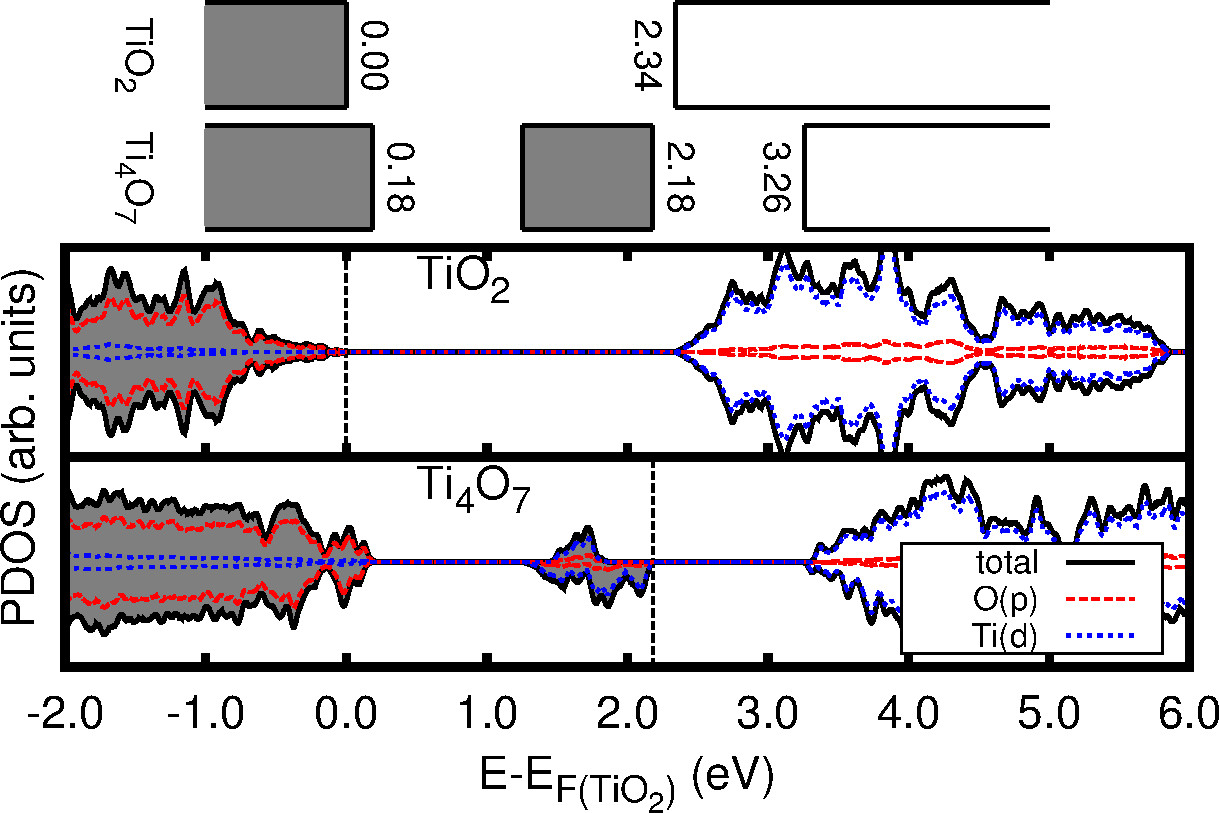
\includegraphics[width=0.8\columnwidth]{img/pdos-bo.jpg}
   \caption{PDOS of TiO${}_2$ rutile and Ti${}_4$O${}_7$. Gray shaded areas denote the occupied levels (below $E_F$, which is highlighted by the dotted vertical lines) and the two spin components are pictured by positive and negative values along the vertical axis. The upper panel shows the band alignment between the two materials.}
   \label{fig:pdos-bo} 
  \end{center}
 \end{figure}
\end{center}

Further evidence of the separation between VBM (more precisely, the Ti$_4$O$_7$ IB) and CBM by the interface is presented in the form of real-space projections of these frontier orbitals, given in figure \ref{fig:parchg-bo}. These projections are performed for the last occupied (VBM) and first unoccupied (CBM) electronic bands, using only the $\Gamma$ point eigenfunctions. From these projections it is possible to see that, while the VBM is mainly located on the Ti atoms of the Ti$_4$O$_7$ side which are close to the interface plane (presenting a small contribution of some Ti atoms of the TiO$_2$ structure), the CBM is delocalized over the same atomic species on the other side. As both levels present Ti(d) character, some degree of hybridization may be responsible for the contribution of the TiO$_2$ part to the VBM. The length of the $c$ vector also seemed to be of some influence in that result, as test calculations using a smaller supercell (the $c$ vector was half the size) present a higher degree of hybridization. Therefore, it is expected that in the limit of $c \rightarrow \infty$ the orbitals will be fully separated on the two phases.
\begin{center}
 \begin{figure}[ht!]
   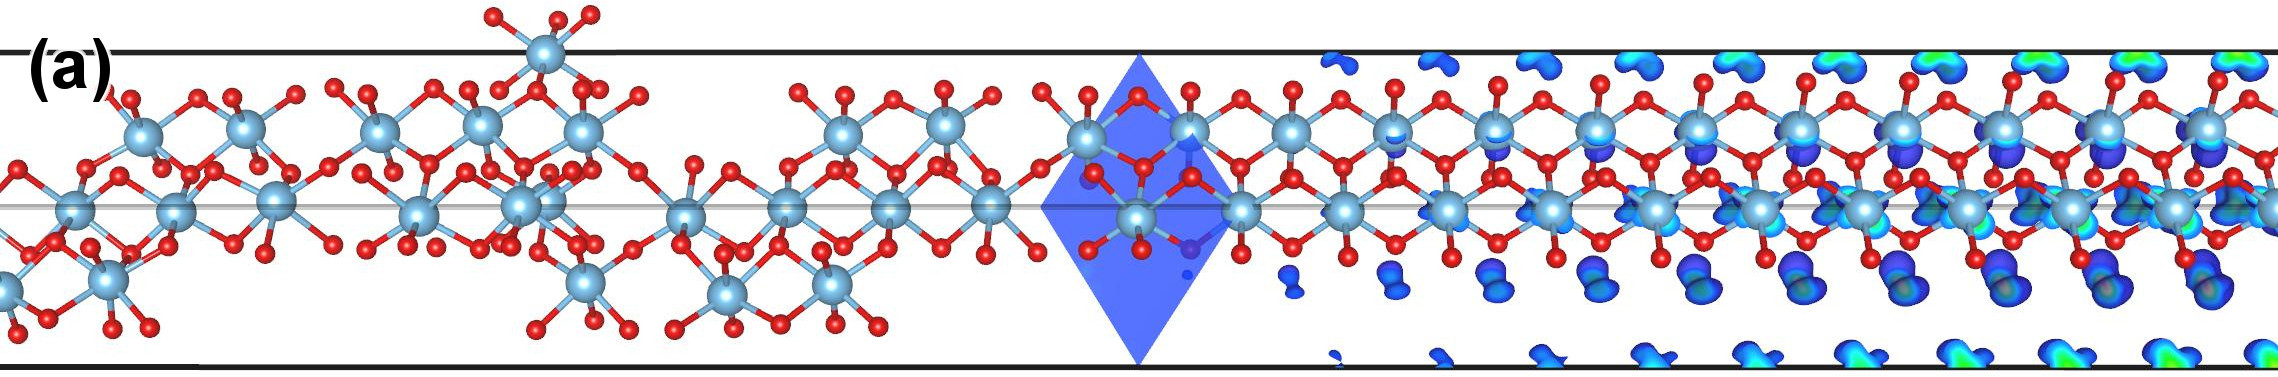
\includegraphics[width=\columnwidth]{img/parchg-cbm-gamma-ti4o7-tio2-new.jpg}
   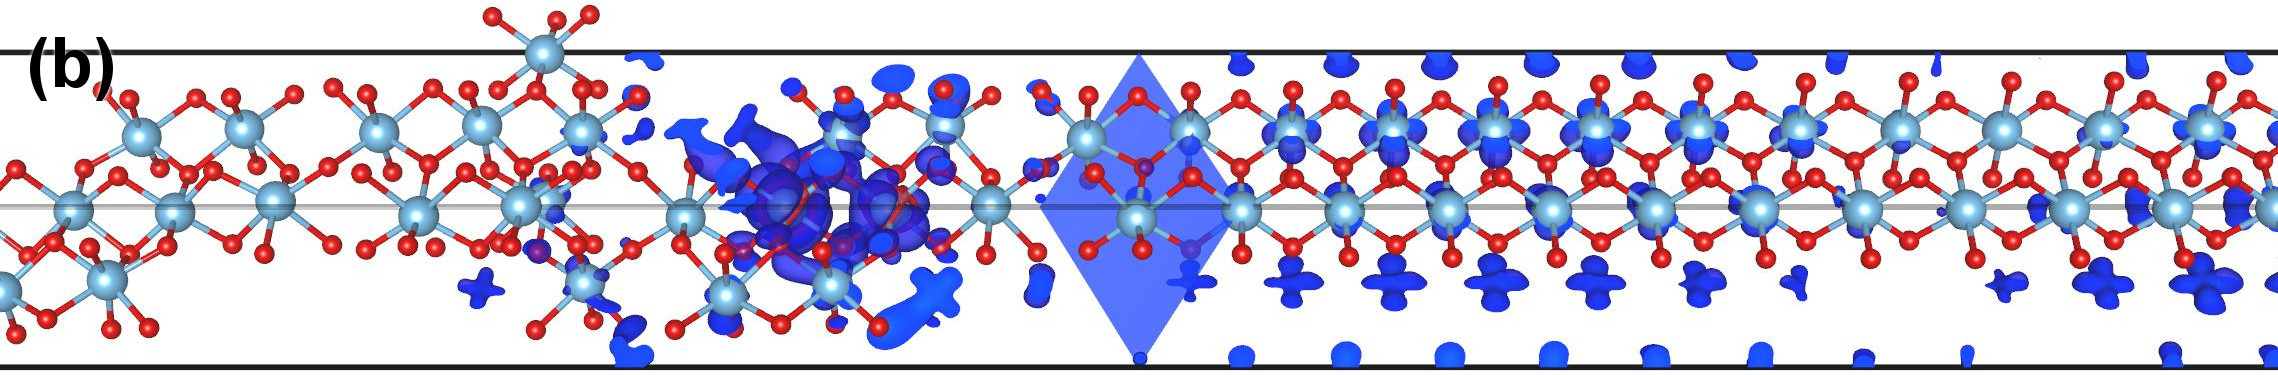
\includegraphics[width=\columnwidth]{img/parchg-vbm-gamma-ti4o7-tio2-new.jpg}
  \caption{Projected charge density for the (a) CBM and (b) VBM of the Ti${}_4$O${}_7$-TiO${}_2$ interface after ionic relaxation. The yellow plane features the interface region of the superstructure, being composed of Ti${}_4$O${}_7$ to the left and TiO${}_2$ to the right.}
  \label{fig:parchg-bo}
 \end{figure}
\end{center}

In conclusion, the results presented show that the IB lies inside the TiO$_2$ bandgap, close to the CM of this compound. This is type II band alignment, where the CB is in one material and the VB (in our case, it is the IB, which is the last occupied level) in the other. This suggests that electrons may be excited from Ti$_4$O$_7$ IB by means of an external perturbation, \textit{e. g.} an electric field of local heating in the active layer of the memristor, to the CB of the TiO$_2$ matrix, thus acting as dopants to this last material. This is a strong evidence of the role of the electronic processes in the memristive phenomena. It is important to emphasize that at this point no dynamical processes were considered: the band offset only is a static feature, but already capable of unraveling important aspects of the memristor that have never been probed before. All results presented in this section were published in Physical Review Applied \cite{Padilha2015}, and the article is attached in appendix \ref{sec:app-pub}.       %chap 3
\chapter{Charge States}
\label{chap:charges}

The results presented in the two previous chapters show that the Ti$_n$O$_{2n-1}$ ($n = 4, 5$) Magnéli phases present an intermediate band (IB) that can act as a $n$-dopant to the TiO$_2$ layer of memristors. This is analogous to the situation where point defects are present in the same stoichiometric structure: the introduction of both the oxygen vacancy ($V_{\text{O}}$) and the interstitial titanium (Ti$_i$) leads to localized levels inside the bandgap \cite{Janotti2010,Lee2012}, usually referred to as \textit{defect levels}. DFT methods are routinely used to assess the stability of such defect levels, by calculating formation enthalpies, via the supercell approach \cite{Haldane1976,Zhang2000,Lany2007}.

In this chapter we use the same methodology to study the stability of the oxygen-deficient phases of TiO$_2$. Indeed, these calculations are not restricted to point defects: they are basically a thermodynamical approach for any reaction, even if the final products present a different number of particles---either atoms or electrons---given that these particles are exchanged with reservoirs that are kept at a constant chemical potential. Reports on the thermochemistry \cite{Liborio2008,Harada2010}, electrical properties \cite{Bartholomew1969}, and electronic structure \cite{Liborio2009,Weissmann2011,Leonov2006} of these systems are available, but the possibility of electronically charging them is unexplored territory. This kind of study is important in our case, where these materials are immersed inside the active layer of memristors, which is in turn subjected to an external voltage, thus, exchange of electrons with a reservoir, \textit{e. g.} the metallic electrodes, must be taken into account.

Surprisingly, for this material, the amount of charge that can be exchanged with this electron reservoir is quite large. Comparison with supercapacitors---mainly composed of oxide thin films capable of charge storage due to defects \cite{Young2015,Simon2008}---shows that these oxygen-deficient materials might be important raw materials for this application due to the fact that their electronic structure \textit{mimics} what is observed for point defects in TiO$_2$. For this reason, we propose the term \textit{pseudodefects} for these structures, owing to the fact that no defects are present in this case but the bulk materials behave as if they contained defects.

The use of the oxygen-deficient phases of TiO$_2$ is proposed by us as raw materials for supercapacitors within a charge storage application. A behavior similar to charge switching levels \cite{Young2015}, which are mainly due to point defects in semiconductor structures and can be occupied and de-occupied by an external perturbation is proposed.

\section{Chemistry of Ti$_n$O$_{2n-1}$ phases}
\label{sec:formation}

The extraction of oxygen from TiO$_2$ can described by two processes: either the removal of oxygen atoms and formation of $V_{\text{O}}$'s or the insertion of titanium atoms as Ti$_i$'s,
\begin{align}
	n\text{TiO}_2 + V_{\text{O}} & \rightarrow \text{Ti}_n\text{O}_{2n-1} \label{eq:vacancy} \\
    (2n-1)\text{TiO}_2 + \text{Ti}_{\text{i}} & \rightarrow 2\text{Ti}_n\text{O}_{2n-1}. \label{eq:interstitial}
\end{align}
In both cases, the Ti:O ratio deviates from the stoichiometric value 0.5, which can be interpreted as the limit $n \rightarrow \infty$. For the first case, given by equation \ref{eq:vacancy}, the shear planes in the TiO$_2$ structure (see figure \ref{fig:ti4o7-struct}) are composed by $V_{\text{O}}$'s which are inserted in the structure via loss of oxygen. On the other hand, equation \ref{eq:interstitial} describes the formation of these planes as caused by the insertion of Ti$_i$. To choose which process best describes the formation of the Magnéli phases, two key observations were made. First, the vector $[0\bar{1}1]$ used to derive the Ti$_n$O$_{2n-1}$ Magnéli phase from the TiO$_2$ structure (see equation \ref{eq:displ}) is a Bravais vector of the oxygen subnet. This means this vector connects two equivalent oxygen sites in the rutile structure, as depicted in figure \ref{fig:rutile-vector}, thus, the operation used to derive the Magnéli structure from the rutile one leaves the oxygen subnet unchanged, \textit{i.\ e.} the oxygen's positions are invariant with respect to that operation.
\begin{center}
 \begin{figure}[ht!]
  \begin{center}
   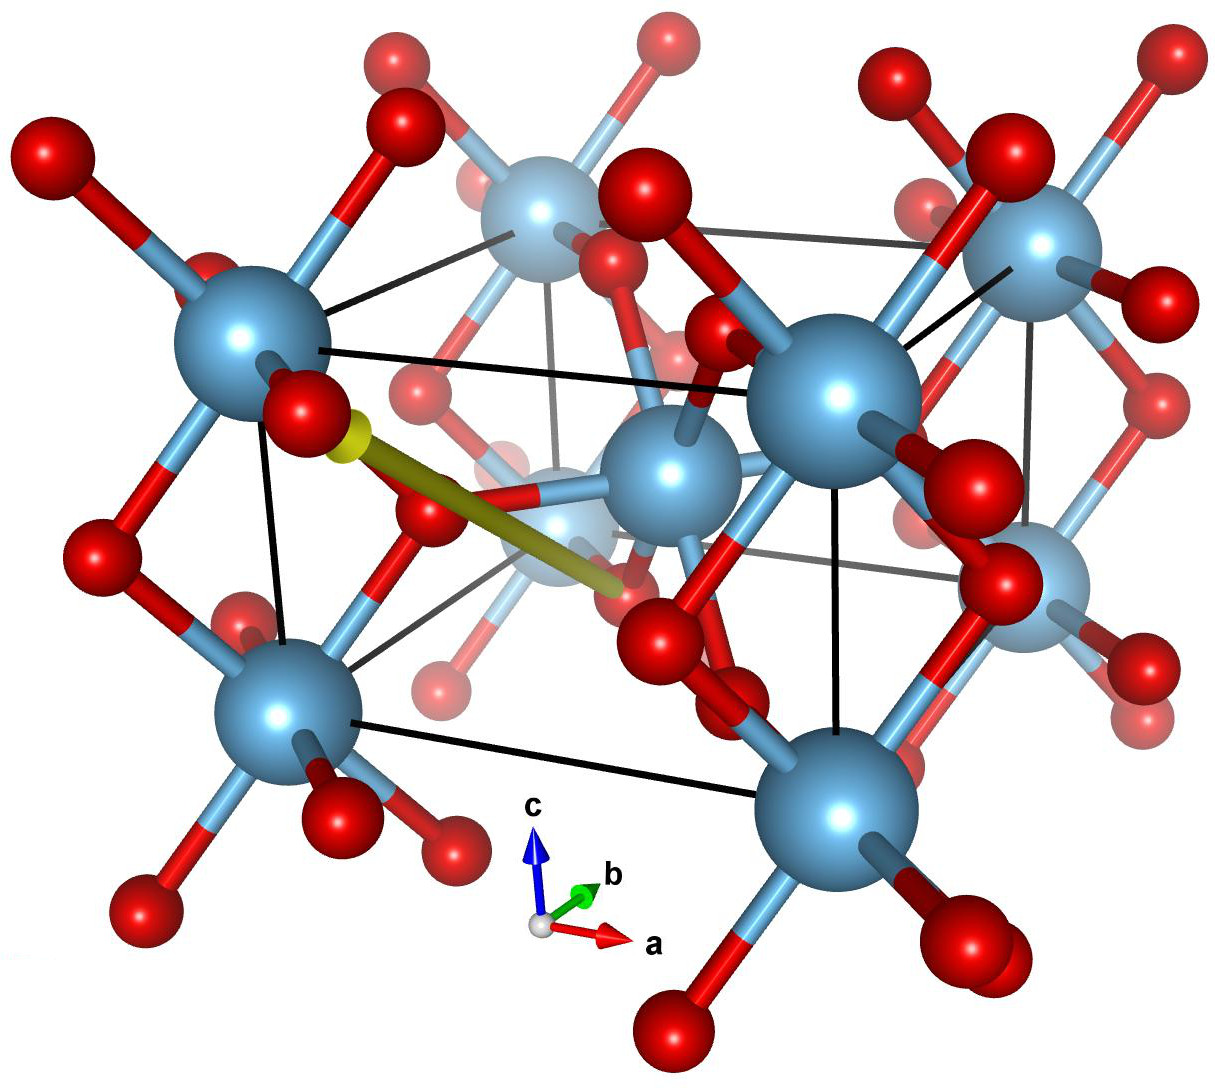
\includegraphics[width=0.45\textwidth]{img/TiO2-rutile-vector.jpg}
   \caption{Unit cell of TiO$_2$-rutile. The $[0\bar{1}1]$ vector, connecting two equivalent oxygen sites, is featured in yellow.}
   \label{fig:rutile-vector} 
  \end{center}
 \end{figure}
\end{center}

The second observation is that in the resulting Magnéli structure, after performing the operations given by equations \ref{eq:transf} and \ref{eq:displ}, some titanium atoms are displaced to interstitial positions with respect to neighboring Ti chains. This can be better visualized in figures \ref{fig:structures-c-prl} (a) and (b), where in the first case, for the TiO$_2$ structure, one can see straight Ti chains along the $c$ vector while in the second case, the Ti$_4$O$_7$ Magnéli structure presents discontinuities in the same chains where interstitial atoms are present. An important detail is that the Ti chains are periodically displaced as if the Ti atoms at their ends were in interstitial positions---and this is exactly where one finds the shear planes---with respect to the neighboring chains along the $c$ direction.
\begin{center}
 \begin{figure}[ht!]
  \begin{center}
   \includegraphics[width=0.45\textwidth]{img/TiO2-c-prl.jpg}
   \includegraphics[width=0.45\textwidth]{img/Ti4O7-c-prl.jpg}
   \caption{Structures of (a) TiO$_2$-rutile, and (b) Ti$_4$O$_7$ Magnéli view along the $c$ axis.}
   \label{fig:structures-c-prl} 
  \end{center}
 \end{figure}
\end{center}

These observations are crucial to determine that it is indeed equation \ref{eq:interstitial} which best describes the formation of the Magnéli phases, thus, the whole process can be regarded as the insertion of Ti atoms into the rutile structure.

\section{Formation Enthalpies}
\label{sec:formation}

For the calculation of the formation enthalpies $\Delta H_f^D$ for the Ti$_2$O$_3$-corundum, and Ti$_4$O$_7$ and Ti$_5$O$_9$ Magnéli phases, reservoirs of atoms at constant chemical potential $\mu_{\alpha}$ ($\alpha = \text{Ti}, \text{O}$) and electrons with the potential at $E_F$ were considered, and the unit cell was kept fixed while ionic relaxation was allowed. The expression for $\Delta H_f^D$ with respect to TiO$_2$-rutile, the host material, is given by,
\begin{align}
	\label{eq:e-form-isolated}
	\Delta H_f^D (E_F, \mu, q) &= E_D(q) - E_H + \sum_{\alpha} m_{\alpha} \mu_{\alpha} + \nonumber \\
							   &+ q (E_F + E_{VBM} + \Delta V),
\end{align}
where $E_H$ and $E_D(q)$ stands for the total energy of the system before (TiO$_2$) and after (Ti$_n$O$_{2n-1}$) exchange of $m_{\alpha}$ atoms and $q$ electrons with the respective reservoirs. VBM energy ($E_{VBM}$) is obtained from the bulk TiO$_2$ while $\Delta V$ is an energy shift obtained from core level eigenvalues. 

\begin{center}
 \begin{figure}[ht!]
  \begin{center}
   \includegraphics[width=0.75\textwidth]{img/e-form-all.jpg}
   \caption{Formation enthalpies for (a) Ti$_2$O$_3$, (b) Ti$_4$O$_7$, (c) Ti$_5$O$_9$, and (d) Ti$_i$ point defect in TiO$_2$-rutile. Each line is the plot of the formation enthalpy for a different charge state, which is the slope, according to equation \ref{eq:e-form-isolated}. The thick black lines feature the lowest energy for each occupation across the bandgap ($E_F$) while the charge transitions are featured by the black arrows.}
   \label{fig:e-form-full} 
  \end{center}
 \end{figure}
\end{center}

According to the discussion in the previous section, in this case one should consider the case where only Ti atoms are inserted into the structure, thus, $\alpha = \text{Ti}$ and $m_{\alpha} = +1$ for the unit cell used in our calculations. This quantity is plotted for each charge state from neutral up to $+4$, given that Ti atoms present oxidation numbers ranging in this interval. The results for the three oxygen-deficient phases are compared with the same quantity obtained for the Ti$_i$ point defect from the literature \cite{Lee2012}, and are presented in figure \ref{fig:e-form-full}. O-rich and Ti-rich conditions are the limiting cases for the $\mu_{\text{Ti}}$, which are given by the stability condition.

From these graphs it is noticeable that Ti$_2$O$_3$ presents a fully ionized state ($q = +4$) as the most stable one across the whole span of the bandgap. This means that, when in the vicinity of TiO$_2$-rutile, this compound is stabilized by donating its four electrons per unit cell. While the same situation happens for most of the bandgap, in the case of Ti$_4$O$_7$ and Ti$_5$O$_9$ there is a transition from $+4$ to neutral state close to $E_{CBM}$: $\varepsilon(+4/0) = E_{CBM} - 0.36$ eV and 0.48 eV respectively. This is very similar to what happens in the case of Ti$_i$, where the same charge transition lies close to the same region: $\varepsilon(+4/0) = E_{CBM} - 0.29$ eV. Thus, these oxygen-deficient structures, which present no crystallographic defects---these are new crystals---behave similarly to Ti$_i$ point defects from an electronic structure point of view. For this reason, we choose to refer to these systems as containing \textit{pseudodefects}. Moreover, the abrupt transition from  $+4$ to neutral state and the large structural relaxation present is a strong evidence of a negative-$U$ behavior \cite{Watkins1984}.

\section{Charge storage}
\label{sec:charge-storage}

The charged states in the Ti$_4$O$_7$ and Ti$_5$O$_9$ structures were investigated by means of the PDOS, presented in figure \ref{fig:pdos-charged}. For each charge state a graph was plotted aiming to understand the changes in the electronic levels due to charging. It is possible to see that the electrons are removed from an \textit{intermediate band} inside the bandgap. As electrons are removed, the most energetic occupied level increases in energy. This effect is more pronounced in the Ti$_4$O$_7$ PDOS but still present in the Ti$_5$O$_9$ case. The consequence of that increase is that the system will switch from the neutral state directly to $+4$ state as long as the Fermi energy is enough lowered by an external perturbation, for example an electrode subject to a given potential.
\begin{center}
 \begin{figure}[ht!]
  \begin{center}
   \includegraphics[width=0.45\textwidth]{img/dos-ti4o7-prl-ef.jpg}
   \includegraphics[width=0.45\textwidth]{img/dos-ti5o9-prl-ef.jpg}
   \caption{PDOS for all charge states of (a) Ti$_4$O$_7$, and (b) Ti$_5$O$_9$. The full black line is the total DOS while the red dashed line is the Ti(d) contribution. The positive and negative values along the vertical axis are the spin components, the vertical red line is the last occupied level and the dashed blue vertical line is the TiO$_2$ CBM. Energies are referenced from the TiO$_2$ VBM.}
   \label{fig:pdos-charged} 
  \end{center}
 \end{figure}
\end{center}

In fact, 3d transition metal-related defects in semiconductors exhibit multiple charge states \cite{Haldane1976}, even in the case where these defects are extended \cite{Raebiger2014}. Cation defects in MnO$_2$ where reported to introduce switching states, which could be used to store charge \cite{Young2015}. In the case of the Magnéli phases presented here, the same switching states are present, but due to an intermediate band introduced by pseudodefects, instead of localized states introduced by point defects. The real-space projection of the intermediate band is presented in figure \ref{fig:ti5o9-parchg-prl}, where it is possible to see that the band is delocalized over several Ti atoms of the structure.
\begin{center}
 \begin{figure}[ht!]
  \begin{center}
   \includegraphics[width=0.18\textwidth]{img/ti5o9-q0-parchg-prl.jpg}
   \includegraphics[width=0.18\textwidth]{img/ti5o9-q1-parchg-prl.jpg}
   \includegraphics[width=0.18\textwidth]{img/ti5o9-q2-parchg-prl.jpg}
   \includegraphics[width=0.18\textwidth]{img/ti5o9-q3-parchg-prl.jpg}
   \includegraphics[width=0.18\textwidth]{img/ti5o9-q4-parchg-prl.jpg}
   \caption{Real-space projection of the intermediate band of Ti$_5$O$_9$ for all studied charge states. The isosurface chosen was $10^{-2}e\cdot \text{Bohr}^{-3}$ while the energy range was $E_F - 1.5 \, \text{eV} < E < E_F$. For the $+4$ state the structure is presented only for completion, once it presents no intermediate band.}
   \label{fig:ti5o9-parchg-prl} 
  \end{center}
 \end{figure}
\end{center}

In conclusion, these systems could be charged and de-charged if a proper setup of electrodes is provided, just as it is the case of the memristors. The switching is then closely related to this charge storage mechanism, and additionally, a charge storage application is possible. Given the fact that the Magnéli phases studied here can donate 4 electrons per unit cell, we estimate that the maximum charge storage capability of a device made of these materials operating at 1 V is 600 F/g for Ti$_4$O$_7$ and 500 F/g for Ti$_5$O$_9$, which places these devices as possible supercapacitors. These results have been submitted for publication and the manuscript is attached in appendix \ref{sec:app-sub}.
     %chap 4
\chapter{Band Bendings}
\label{chap:bandbend}

At this point we begin to have a fairly clear picture of the TiO$_2$-based memristor: the oxygen-deficient phases that arise inside the active layer of the device are responsible for a new ingredient, the intermediate band, which in turn can be charged and de-charged and moreover, $n$-dope the surrounding TiO$_2$ structure. This is enough evidence to consider an electronic model for memristors. In fact, a very similar model has already been proposed for gold impurities inside a SiO$_2$ thin film by Simmons \cite{Simmons1967} long before the discussion about the memristor became popular. Experimental reports at nearly the same time also claim that the transport phenomena could be related to space charge conduction on oxide thin films \cite{Argall1968,Chopra1965}.

However, the so-called \textit{voltage-time dilemma} for purely electronic models claim that the average lifetime of the different charge states---and consequent different resistance states---would be much shorted than the retention times reported \cite{Schroeder2010}. For this reason, many models based on the ionic drift-diffusion of impurities inside the memristor were proposed and became popular among experimentalists. Ielmini \textit{et al.} proposed a \textit{field- and/or temperature-enhanced acceleration} model for ions, which could form and dissolve a conductive channel inside a HfO$_2$ memristor \cite{Ielmini2011,Ielmini2012}. %Curiously, the timescale obtained by direct or indirect measurements for these processes is of the order of seconds or minutes \cite{Yang2014,Kudo2014}, while the reported switching times can reach nanoseconds or even picoseconds \cite{Pan2014}.

The key point is that in most of the claims supporting the ionic drift models and criticizing the electronic models, the profile of the potential energy inside the active region of memristors is assumed to be of a certain shape. For the voltage-time dilemma, typical metal-insulator \textit{band bendings} are assumed as solutions to Poisson equation and the resulting barriers are approximated by triangles or trapezoids \cite{Schroeder2010}, while for the accelerated ionic motion models the potential is assumed to be a straight line (constant electric field across the active region) \cite{Ielmini2011,Ielmini2012}. Unfortunately, no explicit solution of the Poisson equation is presented in the literature. The role of the electronic processes in the switching is readily discarded, but there is no reason, in principle, to consider that either the electronic models or the ionic models should be considered as the only driving force of the mechanism. The assessment of the importance of the electronic contribution is the subject of this chapter, where the solution of the Poisson equation for fixed ions is presented.

\section{Solving the Poisson equation}
\label{sec:poisson}

As a first approximation, the memristor can be modeled as a 1D device\footnote{Owing to periodic boundary conditions in the transverse ($x$ and $y$) coordinates, the potential is constant in these directions.}, thus, the total energy of the system can be written as a functional of the electrostatic potential $\phi$,
\begin{equation}
	F[\phi(z)] = \int_a^b \mathrm{d}z \left[ \frac{1}{2}\left( \frac{\mathrm{d}\phi}{\mathrm{d}z}\right)^2+\frac{\phi \rho}{\epsilon \epsilon_0}\right],
	\label{eq:poisson}
\end{equation}
where $z$ is the direction perpendicular to the metal/semiconductor interface, $\rho$ is the charge density along this direction, and $\epsilon$ and $\epsilon_0$ are the relative and vacuum permittivities respectively. This expression comprises the energy density of the electric field ($|\vec{E}|^2=(\mathrm{d}\phi/\mathrm{d}z)^2$) and the same quantity due to the interaction between the charge density and the potential. The function $\phi$ that minimizes \ref{eq:poisson} is the solution to the Poisson equation, \textit{i. e.} the electrostatic potential. The Euler-Lagrange equation for this functional is
\begin{equation}
	\frac{\mathrm{d}^2 \phi}{\mathrm{d}z^2}=\frac{\rho}{\epsilon \epsilon_0} + \frac{\phi}{\epsilon \epsilon_0}\frac{\partial \rho}{\partial \phi}.
	\label{eq:euller-lagrange}
\end{equation}

Owing to the fact that the charges are not fixed inside the active layer of the memristor, $\rho$ is a functional of $\phi$, \textit{i.e.}, $\rho = \rho[\phi(z),z]$, and its expression is given by
\begin{equation}
	\rho = -n_e + n_h + N_D(q_D - n_D)
	\label{eq:charge-density}
\end{equation}
where $N_D$, and $n_D$ are respectively the concentration, and the charge state of defects inside the active region, $q_D$ the number of electrons trapped in these defects, while $n_e$ and $n_h$ are the concentrations of electrons in the CB and holes in the VB respectively, which are given by
\begin{equation}
	n_e = \int_{\phi}^{+\infty} \frac{g_c(\varepsilon)\mathrm{d}\varepsilon}{e^{\nicefrac{\varepsilon}{kT}}+1}, \qquad
	n_h = \int_{-\infty}^{\phi-E_g} \frac{g_v(\varepsilon)\mathrm{d}\varepsilon}{e^{\nicefrac{-\varepsilon}{kT}}+1},
	\label{eq:e-h-dens}
\end{equation}
where $k$ is Boltzmann's constant, $T$ is the temperature, $\varepsilon$ is the energy, and $g_c$ and $g_v$ are the density of states for the electrons in CB and holes in VB respectively, given by
\begin{equation}
	g_c(\varepsilon) = \frac{m_c^{*\nicefrac{3}{2}}}{\hbar^3 \pi^2}\sqrt{2(\varepsilon-\phi)}, \qquad
	g_v(\varepsilon) = \frac{m_v^{*\nicefrac{3}{2}}}{\hbar^3 \pi^2}\sqrt{2(\phi-E_g-\varepsilon)},
\end{equation}
where $m_c^*$ and $m_v^*$ are the effective masses of electrons and holes respectively, $\hbar = \nicefrac{h}{2\pi}$ is Planck's constant and $E_g$ is the bandgap energy. Finally, the occupation of the defect levels is given by a Boltzmann distribution,
\begin{equation}
	n_D = \frac{\sum_j N_j e^{\nicefrac{-\varepsilon_j}{kT}}}{\sum_j e^{\nicefrac{-\varepsilon_j}{kT}}}.
\end{equation}
where $\varepsilon_j$ and $N_j$ are the energy and number of electrons in state $j$ within the bandgap. Equation \ref{eq:euller-lagrange} can be discretized by rewriting the second derivative as
\begin{equation}
	\frac{\mathrm{d}^2 \phi}{\mathrm{d}z^2} \approx \frac{\phi_{i-1}-2\phi_i+\phi_{i+1}}{h^2}, \qquad 1 \leq i \leq N,
\end{equation}
where $h = \nicefrac{(b-a)}{N}$ is the finite element in a real-space grid, $\phi_j = \phi(z_j)$ is the electrostatic potential in the $j$-th grid point, and imposing Dirichlet boundary conditions $\phi_0 = \phi(a) = \phi_a$, and $\phi_{N+1} = \phi(b) = \phi_b$, which correspond to the Schottky barriers at the insulator/metal interfaces, the final result can be written in matrix form,
\begin{equation}
\tiny
	\left[ 
		\begin{array}{cccccc}
 			-\frac{2}{h^2}-\frac{\partial_{\phi} \rho_1}{\epsilon \epsilon_0} & \frac{1}{h^2} & 0 & 0 & \cdots & 0 \\
 			\frac{1}{h^2} & -\frac{2}{h^2}-\frac{\partial_{\phi} \rho_2}{\epsilon \epsilon_0} & \frac{1}{h^2} & 0 & \cdots & 0 \\
 			\vdots & \vdots &  & &  & \vdots \\
 			0 & 0 & \cdots & \frac{1}{h^2} & -\frac{2}{h^2}-\frac{\partial_{\phi} \rho_{N-1}}{\epsilon \epsilon_0} & \frac{1}{h^2} \\
 			0 & 0 & \cdots & 0 & \frac{1}{h^2} & -\frac{2}{h^2}-\frac{\partial_{\phi} \rho_N}{\epsilon \epsilon_0}
		\end{array} 
	\right] 
	\left[
		\begin{array}{c} 
			\phi_1 \\ 
			\phi_2 \\ 
			\vdots \\ 
			\phi_{N-1} \\
			\phi_N 
		\end{array} 
	\right] 
	= 
	\left[
		\begin{array}{c}
			\frac{\rho_1}{\epsilon \epsilon_0} - \phi_a \\ 
			\frac{\rho_2}{\epsilon \epsilon_0} \\ 
			\vdots \\ 
			\frac{\rho_{N-1}}{\epsilon \epsilon_0} \\
			\frac{\rho_N}{\epsilon \epsilon_0} - \phi_b
		\end{array}
	\right]
	\normalsize
	\label{eq:matrix-euller-lagrange}
\end{equation}
where the derivatives $\partial_{\phi} \rho_i =\nicefrac{\partial \rho_i}{\partial \phi}$ are obtained numerically by finite differences. According to equations \ref{eq:charge-density} and \ref{eq:e-h-dens}, the charge density is a functional of the potential, $\rho = \rho[z,\phi(z)]$, thus, we start from a parabolic \textit{ansatz} for $\phi$ and evaluate $\rho$ by numerical integration.
\begin{center}
  \begin{figure}[h!]
    \begin{center}
      \includegraphics[width=0.8\textwidth]{img/switch-2x2.jpg}    
      \caption{Multiple solutions of the Poisson equation for a 20 nm wide memristor. The curves are the potential barrier for charges to flow through the device. The dashed horizontal line depicts the Fermi Level. The HRS is featured in the left column while the LRS for the corresponding voltage is featured in the right column.} 
      \label{fig:multiple-poisson} 
    \end{center}
  \end{figure}
\end{center}

Using these results in equation \ref{eq:matrix-euller-lagrange} we solve the system numerically \footnote{By use of a Lapack routine \cite{lapack}} and obtain the first iteration, subsequently calculating the potential in every point of the real-space grid $\phi_j$. This result allows the calculation of a new charge density by integration of equations \ref{eq:e-h-dens} and substitution into \ref{eq:charge-density}. The \textit{self-consistent solution} to this set of equations is obtained by repeating this process until the Dirichlet energy (equation \ref{eq:poisson}) is converged. The resulting $\phi$ are the potential barriers for electrons to flow through the active region, which in this case presents multiple stable solutions, \textit{i. e.} there are two solutions, one is the High Resistance State (HRS) while the other is the Low Resistance State (LRS), for a given potential, as shown in figure \ref{fig:multiple-poisson}. 
\begin{center}
  \begin{figure}[h!]
    \begin{center}
      \includegraphics[width=0.9\textwidth]{img/switch-4x3.jpg}    
      \caption{Snapshots of the resulting potential energy barriers for a 20 nm wide memristor. The dashed horizontal line depicts the Fermi Level. Each step is an increase or decrease of 0.1 V, which is basically the height of the Schottky barrier at the electrode at the origin.} 
      \label{fig:potentials} 
    \end{center}
  \end{figure}
\end{center}

More results obtained from the code implemented by Dr. Raebiger are presented in figure \ref{fig:potentials}. For each run the dielectric Schottky barrier at the right electrode is kept fixed at 1 V ($\phi_b = 1$) while the left electrode barrier is varied according to the voltage. The first switch takes place at step 12, when $\phi$ touches the Fermi level and the device goes from HRS to LRS. From step 17 to step 52, the left barrier $\phi_a$ is raised\footnote{Our convention is that the voltage $V = 0$ if the Schottky barrier $\phi_a = 1$ V. When the voltage is raised the barrier is lowered and vice-versa.} and in step 53 $\phi$ \textit{detaches} from the Fermi level abruptly: this is the switching from LRS to HRS.
\begin{center}
  \begin{figure}[h!]
    \begin{center}
      \includegraphics[width=0.8\textwidth]{img/charge-energy.jpg}    
      \caption{Total energy $F$ (given by equation \ref{eq:poisson}) for defect scenarios: (a) i) a homogeneous concentration of $5 \cdot 10^{-3} \, \text{nm}^{-3}$ of $V_{\text{O}}$, and (c) ii) homogeneous concentration of $5 \cdot 10^{-3} \, \text{nm}^{-3}$ of Ti$_i$ together with $2.5 \cdot 10^{-3} \, \text{nm}^{-3}$ of $V_{\text{O}}$. Total charge $Q$ for scenarios: (b) i), and (d) ii). Switch between LRS and HRS is shown by arrows labeled 1 and 2, while arrows 3 and 4 depict the switching to and from the IRS. The inset in (d) shows the hysteresis loop for the switching between HRS and IRS.} 
      \label{fig:charge-energy} 
    \end{center}
  \end{figure}
\end{center}

The total charge $Q$, obtained by integrating the resulting $\rho$ on the real-space grid, is shown to be distinct for the two solutions, as well as the Dirichlet (or total) energy $F$ of the system, given by equation \ref{eq:poisson}, as presented in figure \ref{fig:charge-energy} for two homogeneous defect concentration scenarios: i) $5 \cdot 10^{-3} \, \text{nm}^{-3}$ of oxygen vacancies ($V_{\text{O}}$), and ii) $5 \cdot 10^{-3} \, \text{nm}^{-3}$ of titanium interstitials (Ti$_i$) with $2.5 \cdot 10^{-3} \, \text{nm}^{-3}$ of $V_{\text{O}}$. An intermediate resistance state (IRS) is detected in scenario ii), due to the multiple defect states present within the bandgap. In these graphs one can see two [defect scenario i)] or three [defect scenario ii)] distinct values of energy or charge for each value of the applied voltage. By raising or lowering the voltage the distinct curves overlap and the switching occurs. Arrows 1 and 2 are respectively the reset and set processes in defect scenario i) [figure \ref{fig:charge-energy} (a) and (b)], while arrows 1 and 2 play the same role for defect scenario ii) with an additional hysteresis loop from HRS to IRS and back described by arrows 3 and 4 [figure \ref{fig:charge-energy} (c) and (d)]. While for HRS and IRS the total charge is slightly positive for the most part of the switching cycle, the LRS shows an accumulation of negative charge. This is consistent with a scenario where the HRS and IRS present fully or partially ionized defect levels and poor conduction, while the LRS is such that band conduction is possible owing to the presence of electrons in the CB of the material.
\begin{center}
  \begin{figure}[h!]
    \begin{center}
      \includegraphics[width=0.8\textwidth]{img/field.jpg}    
      \caption{Potentials $\phi$ and corresponding electric fields $E$ for HRS (red), IRS (orange), and LRS (blue) in defect scenario ii) and different applied voltages. The gray dashed line depicts the constant electric field $E_0 = V/L$ for comparison.} 
      \label{fig:field-pot} 
    \end{center}
  \end{figure}
\end{center}

The electric field $E = \partial \phi / \partial z$\footnote{Notice that the signal convention is not the usual here due to the fact that we are interested in the barriers for electrons.} and corresponding potential $\phi$ for defect scenario ii) are shown in figure \ref{fig:field-pot}, where one can see huge electric fields close to the electrodes. These fields are responsible for expelling electrons from the active media while the system is in HRS and doing the opposite in the LRS and IRS. See for example figure \ref{fig:field-pot} (a) where $E > 0$ close to the left electrode and $E < 0$ close to the opposing electrode for the HRS state and vice-versa for LRS and IRS. In this situation, the HRS state responds to an insertion of electrons by expelling them, and the LRS does the opposite: these are stationary solutions. Of course, the large values of the electric field close to the electrodes might lead to ionic migration, or even to the breakdown of the material. Such extreme situation might be avoided by a rearrangement of the defects in these interfacial layers, as it is detected by experiments \cite{Kwon2010,Szot2011,HwanKim2011}.
\begin{center}
  \begin{figure}[h!]
    \begin{center}
      \includegraphics[width=0.8\textwidth]{img/energy-width.jpg}    
      \caption{Total energy $F$ (solid lines) and its contribution due to the interaction between charge density and potential $F_{\rho} = \int_a^b \mathrm{d}z \left(\nicefrac{\rho \phi}{\epsilon \epsilon_0}\right)$ (dashed lines) as a function of device width $L$. HRS, IRS, and LRS are the red, orange, and blue curves respectively. Defect concentrations are: (a) $1.0 \cdot 10^{-3} \, \text{nm}^{-3}$, (b) $5.0 \cdot 10^{-3} \, \text{nm}^{-3}$, and (c) $1.0 \cdot 10^{-2} \, \text{nm}^{-3}$ of homogeneously distributed $V_{\text{O}}$ and half these values of Ti$_i$.} 
      \label{fig:fxl} 
    \end{center}
  \end{figure}
\end{center}

Finally, the sensitivity to device parameters is assessed for our memristor model. By controlling the width of the device ($L = b - a$) and the concentration of defects ($N_D$), as well as the defect state charge $q_{D,0}$ and energy $E_D$ with respect to CBM, different profiles are obtained. Plots of the total energy $F$ and $F_{\rho} = \int_a^b \mathrm{d}z \left(\nicefrac{\rho \phi}{\epsilon \epsilon_0}\right)$, the contribution to $F$ arising from the interaction between the charge density $\rho$ and the potential $\phi$ with respect to the device width $L$ are shown in Figure \ref{fig:fxl} for various defect concentrations. For higher concentrations, both $F$ and $F_{\rho}$ diverged quickly as the thickness increases, owing to the fact that larger charges are stored inside the device in this case, leading to strong electrostatic repulsion. This shows that the interplay between defect concentration and the thickness of the device might be responsible for the memristive property to arise at the nanoscale. Large defect concentrations, as provided by the Magnéli phases fit in this model. %All results shown here are once more presented in our preprint \cite{Raebiger2014} (appendix \ref{sec:app-sub}).

\section{Electronic Transport}
\label{sec:transport}

The simplest model for the electronic transport across the device consists of scattering and/or tunneling of electrons through a potential energy barrier. Within our first approximation, electrons are regarded as free waves incident, reflected and transmitted across a 1D barrier. The corresponding wavefunctions in the neighboring regions to the active region are
\begin{equation}
	\psi_L(z) = e^{ik_Lz}+re^{-ik_Lz}, \qquad
	\psi_R(z) = te^{ik_Rz},
	\label{eq:wavefunct}
\end{equation}
where $k_{L/R}=\sqrt{\nicefrac{2m}{\hbar^2}(\varepsilon-U_{L/R})}$ are the 1D wave vectors of the electrons in the left and right electrodes respectively, and $\varepsilon$ is the total energy of the electron. 

\begin{center}
  \begin{figure}[h!]
    \begin{center}
      \includegraphics[width=0.6\textwidth]{img/transm-01.jpg}    
      \caption{Diagram of the electron tunneling process across a 1D memristor of width $L$. The potential $U(z)$ is obtained from the Poisson solver while the right electrode potential $U_R$ is kept fixed and the left electrode potential $U_L$ is varied.} 
      \label{fig:transm-01} 
    \end{center}
  \end{figure}
\end{center}

The diagram in figure \ref{fig:transm-01} depicts this situation. According to what was done in the solution of the Poisson equation, the potential in the right electrode is kept fixed for all calculations ($U_R = 1.0$ V) while the potential in the opposite electrode ($U_L$) is changed according to the voltage to which the device is subject. 

The wavefunction in the scattering region is the solution of the 1D single-particle time-independent Schr\"odinger equation
\begin{equation}
	-\frac{\hbar^2}{2m}\frac{\mathrm{d}^2}{\mathrm{d}z^2}\psi(z)+U(z)\psi(z)=\varepsilon \psi(z),
	\label{eq:schrodinger}
\end{equation}
which can be in turn discretized in the same way as it was done in the previous section, 
\begin{equation}
	\frac{\mathrm{d}\psi}{\mathrm{d}z}\approx \frac{\psi_i-\psi_{i-1}}{h}, \qquad 1 \leq i \leq N-1, 
\end{equation}
resulting in a finite-differences equation \cite{NR,King},
\begin{equation}
	\frac{1}{h^2}\psi_{j-1}+\left[ \frac{2m}{\hbar^2} (\varepsilon-U_j) - \frac{2}{h^2}\right] \psi_j + \frac{1}{h^2}\psi_{j+1}=0, \qquad 1 \leq j \leq N - 1,
	\label{eq:finite-diff-schrodinger}
\end{equation}
where $h = \nicefrac{L}{N}$ is one segment of the $N$-positions real-space grid, and $\psi_j = \psi(z_j)$ is the solution to the Schr\"odinger equation for a constant potential $U_j = U(z_j)$ in this segment. Imposing the continuity of the wavefunction at the metal/insulator interfaces $\psi_0=\psi_L(z_0)$, and $\psi_N=\psi_R(z_N)$, as well as for the derivatives $\psi_0'=\psi_L'(z_0)$, and $\psi_N'=\psi_R'(z_N)$, and eliminating $r$ and $t$ from these equations, it is possible to write equation \ref{eq:finite-diff-schrodinger} in matrix form
\begin{equation}
	%\begin{array}{cccc}
	\tiny
		\left[\begin{array}{cccccc}
			-\frac{1}{h}+ik_L & \frac{1}{h} & 0 & \dots & 0 & 0 \\
			\frac{1}{h^2} & k_1^2-\frac{2}{h^2} & \frac{1}{h^2} & \dots & 0 & 0 \\
			\vdots & \vdots & & \ddots & \vdots & \vdots \\
			0 & 0 & \dots & \frac{1}{h^2} & k_{N-1}^2-\frac{2}{h^2} & \frac{1}{h^2} \\
			0 & 0 & \dots & 0 & -\frac{1}{h} & \frac{1}{h}-ik_R
		\end{array}\right]
		\left[\begin{array}{c}
			\psi_0 \\ \psi_1 \\ \vdots \\ \psi_{N-1} \\ \psi_N
		\end{array}\right]
		=
		\left[\begin{array}{c}
			2ik_Le^{ik_Lz_0} \\ 0 \\ \vdots \\ 0 \\ 0
		\end{array}\right]
		\normalsize
		\label{eq:schroedinger-discrete-matrix}
	%\end{array}
\end{equation}
where $k_j^2 = \nicefrac{2m^*}{\hbar^2}(\varepsilon-U_j), 1 \leq j \leq N-1$. This equation is then solved numerically by a Fortran 90 code. The parameters used were $z_0 = 0$, $z_N = L = 20$ nm, the effective mass for electrons in TiO$_2$, $m^* = 0.8m_e$ (from DFT bandstructure calculations) while the values of $\varepsilon$ and $U_L$ were varied. Knowing the value of $\psi$ at the interfaces, it is straightforward to determine $r$ and $t$ from the equations used to impose the continuity of the wavefunction at these regions, $r = \psi_0-1$, $t=\psi_Ne^{-ik_RL}$. Thus, the probability of reflection $R$ and transmission $T$ is obtained by \cite{Cohen-Tannoudji}
\begin{equation}
T(U_{L/R},\varepsilon) = \left|\frac{k_R}{k_L}\right|^2|t|^2, \qquad
R(U_{L/R},\varepsilon) = |r|^2.
\end{equation}

At this point, the current is obtained from Landauer's model for the electronic transport at the nanoscale \cite{Datta}
 \begin{equation}
	I(U_L,U_R) = \frac{2e}{h} \int_{-\infty}^{+\infty}T(\varepsilon,U_{L/R}) \left[f(\varepsilon,U_L,T)-f(\varepsilon,U_R,T)\right] \mathrm{d}\varepsilon
\end{equation}
where $\nicefrac{2e}{h}$ is the quantum of conductance and $f_{L/R}$ are the Fermi-Dirac distributions at the electrodes. The temperature where the calculations took place was $T= 300$ K. The resulting $i \times V$ curve is presented in figure \ref{fig:ixvtheo-01} and it is compared with an experimental curve \cite{Pan2014}. The order of magnitude of the current for both high resistance (HR) and low resistance (LR) is very small in comparison with the experimental curve. A region of negative differential resistance is present for the LRS beyond 0.5 V which can be interpreted as a decrease in occupation in the CB (see Figure \ref{fig:potentials}, steps 17-52). Thus, it is an evidence of other transport mechanisms being responsible for the electronic current in the memristors.
\begin{center}
  \begin{figure}[h!]
    \begin{center}
      \includegraphics[height=5cm]{img/ixv-tunnel.jpg}    
      \includegraphics[height=5cm]{img/pan.jpg}    
      \caption{(a) theoretical and (b) experimental $i \times V$ curves of memristors \cite{Yang2009}. In (a) the blue curve is the LRS while the green one is the HRS.} 
      \label{fig:ixvtheo-01} 
    \end{center}
  \end{figure}
\end{center}

The role of the defect levels was not taken into account for the the transmission. A step in this direction is to consider a defect band inside the bandgap at $E_{CBM}-E_d$, as depicted in figure \ref{fig:ixvtheo-02} (a). In this case, the electrons are allowed to flow through this band in the same way they were considered to cross the CB. In practice, the CB is lowered by $E_d \approx 0.5$ eV in the region where it is higher than this value and considered zero everywhere else. This change led to a much more reasonable theoretical $i \times V$ curve, shown in figure \ref{fig:ixvtheo-02} (b). However, there is still an issue with respect to negative differential resistivity in the region $V > 0.5$ V for both the low and high resistivity curves, being the effect more pronounced for the first case. 
\begin{center}
  \begin{figure}[h!]
    \begin{center}
      \includegraphics[height=4.5cm]{img/defect-band.jpg} 
      \includegraphics[height=4.5cm]{img/ixv-deff.jpg} 
      \caption{(a) sketch of the band bending inside the active layer of a memristor where the defect band is depicted as the dashed segment laying $E_d$ lower than CBM. (b) theoretical $i \times V$ curve obtained after changing the potential. The blue curve is the LRS while the green one is the HRS.} 
      \label{fig:ixvtheo-02} 
    \end{center}
  \end{figure}
\end{center}

In conclusion, the results presented in this chapter indicate that purely electronic mechanisms do play an important role in memristive switching. Using simple 1D models for both the electrostatic potential (solution to the Poisson equation) and the transmission probability (Schr\"odinger equation) we could derive multiple solutions to the memristor's potential barrier, show that these distinct solutions are stable and present a domain of coexistence of these solutions with respect to defect concentrations and device width. Consequently, the electronic current was obtained for to two simple mechanisms: tunneling and band-assisted tunneling. Even though the $i \times V$ curves do not capture all the features of the switching, it is evident that a qualitative agreement is achieved in comparison to experimental results. Still in the purely electronic mechanism picture, the consideration of other electronic transport models might lead to better agreement between the simulated and the experimental curves. Another approach would be the extension of the model to 2D or 3D, by solving both the Poisson equation and the Schr\"odinger equation in these dimensions, in a more realistic situation. The results presented here for the Poisson equation solver were submitted for publication, and the manuscript is attached in appendix \ref{sec:app-sub}.         %chap 5
\chapter{Conclusions}
\label{chap:concludions}

This PhD thesis presents one of the few computational-theoretical approaches to the memristor. By means of a bottom-up strategy we studied the prototypical TiO$_2$-based memristor from the raw materials to the device.

 The raw materials, oxygen-deficient phases of TiO$_2$, namely the corundum structure Ti$_2$O$_3$, the $\alpha-$, $\beta-$, and $\gamma-$Ti$_3$O$_5$, and the Magnéli phases Ti$_4$O$_7$ and Ti$_5$O$_9$ were studied in chapter \ref{chap:raw} with three flavors of DFT methods: a GGA functional, GGA$+U$, and hybrid functional HSE. These calculations revealed the presence of an intermediate band within the bandgap for most of these materials. The most important cases, the Magnéli phases, known to be formed inside the memristor after electroforming, presented a Ti(d) filled band lying close to CBM. Such band can act as a $n-$dopant to the surrounding TiO$_2$, thus changing its electronic properties. This was the first evidence of the importance of the electronic processes taking place inside memristors.

 The TiO$_2$-Ti$_4$O$_7$ interface spans the device, eventually connecting the opposing electrodes. Our band offset calculations in chapter \ref{chap:band-offset} showed the correct position of the intermediate band of the Magnéli phase with respect to the TiO$_2$ CBM. Lying just 160 meV below the TiO$_2$ unoccupied levels, this filled band can act as an electron donor to the TiO$_2$ matrix. This is a strong evidence of the electronic mechanisms being important for the memristive property. The separation of charges between the two structures suggested that a charge transfer might take place.

 Taking into consideration a possible charging and de-charging of the Magnéli phases formed inside the memristors, we studied the stability of these compounds using formation enthalpy calculations in chapter \ref{chap:charges}. The results show that Magnéli phases Ti$_4$O$_7$ and Ti$_5$O$_9$, as well as corundum phase Ti$_2$O$_3$ can be charged due to the presence of charge switching levels within the bandgap. These are exactly the intermediate bands reported in the previous studies. One important point is that when the intermediate band donates all its electrons, these oxygen-deficient phases become insulators. The arguments in favor of electronic switching are further reinforced by this result.

 Finally, a semiclassical picture of the memristor is presented in chapter \ref{chap:bandbend}. By considering a defective TiO$_2$ layer as the active part of the memristor, the Poisson equation was solved numerically by a self-consistent scheme. The fact that the defects inside the oxide could be charged and de-charged led to the fact that multiple solutions to the Poisson equation, \textit{i. e.}, multiple profiles of the potential energy barrier for electrons to cross the device, are possible. Using the calculated potential, the electronic current was calculated numerically and two distinct resistance states were obtained.

 A picture featuring all points studied in this thesis is presented in Figure \ref{fig:mem-concl}. There it is possible to observe all points covered in this project: the raw materials were investigated by DFT calculations of the electronic structure of the oxygen-deficient Ti$_n$O$_{2n-1}$ phases (chapter \ref{chap:raw})as well as the thermodynamic stability of these materials (chapter \ref{chap:charges}); the interface between TiO$_2$ and Ti$_4$O$_7$ was simulated for a better understanding of the band alignment between them (chapter \ref{chap:band-offset}); and finally the Poisson and Schr\"odinger equations were solved for the band bendings and electronic transport in the device (chapter \ref{chap:bandbend}).
 
Summarizing our conclusion is that electronic mechanisms similar to what was proposed by Simmons \cite{Simmons1967} definitely play an important role in resistance switching. As most of the literature focus on ionic drift models, the electronic models do not receive the same attention, but there is no reason to consider both models exclusive. The defects are present in all memristors made of a variety of materials, and in many situations these defects can become charged and affect the electronic properties of the active layer of the device. Of course these models do not exclude each other: there may be a contribution from both the charge and de-charge of defects as well as the migration of ions, but to understand the interplay between these mechanisms one should couple the ionic motion into the Poisson solver. One last remark is that the ionic motion is probably the dominant process during the electroforming step, when the defect concentration increases and thus enables the charging and de-charging of the active layer.

\begin{center}
  \begin{figure}[h!]
    \begin{center}
      \includegraphics[width=0.7\textwidth]{img/memristor-concl-B.jpg}    
      \caption{A bottom-up approach to model the memristor. From the raw materials (Ti$_n$O$_{2n-1}$ phases were studied in chapters \ref{chap:raw} and \ref{chap:charges}), going through the interfaces (band alignment between TiO$_2$ and Ti$_4$O$_7$, chapter \ref{chap:band-offset}), and finally the simulation of the device (solution of Poisson and Schr\"odinger equations, chapter \ref{chap:bandbend}).} 
      \label{fig:mem-concl} 
    \end{center}
  \end{figure}
\end{center}
%The two main perspectives of this work are: i) study of the ionic motion within the active layer. Using minimum-path methods such as the nudged elastic band (NEB) \cite{Henkelman2000a,Henkelman2000b} we want to evaluate the real barriers for ionic motion in the memristive materials. The effects of electric fields and temperature must be taken into account for a correct description of the system \cite{Crehuet2003}. ii) more models for electronic transport in defective semiconductors such as the variable range hopping (VRH) \cite{}. The whole picture should be available when both models for electronic switching and their simultaneous effects are understood in an atomic level.       %chap 6

\renewcommand{\chaptername}{Appendix}	%troca a palavra "Capítulo" por "Apêndice"

\appendix

\chapter{Appendices}

\section{Calculation Details}
\label{sec:app-calc}

As it was stated in the main text, the details for all DFT calculations are provided here. All such calculations were performed using the Vienna \textit{Ab Initio} Simulation Package (\texttt{VASP}) \cite{Kresse1996a,Kresse1996b,Kresse1999,Kresse1993} versions 5.2.1 up to 5.3.5. For further details on the DFT methods we suggest some sources in the literature \cite{FazzioCanutoVianna,Hohenberg_Kohn_64,Thomas,YangParr,Kohn_Sham_65,Fermi_28,Bloch_29,Kresse1996a,Kresse1996b,Capelle2006,Zangwill2014,Jensen,Ihm1979,Blochl1994,Kresse1999,Kresse1993}, once the theory underlying this work is beyond this thesis' scope. All figures of structures were created by the \texttt{VESTA3} software \cite{Momma2011}. In all cases except when explicitly stated, the calculations were performed using the primitive cell obtained by the \texttt{--symmetry} command line option of \texttt{Phonopy} \cite{phonopy}.

The simulations of all materials presented in chapter \ref{chap:raw} were performed using three methods: the GGA PBESol \cite{Perdew2008} and hybrid HSE (20\% of Hartree-Fock exchange)\cite{Heyd2003} functionals (see appendix \ref{sec:app-hybrid}), and the PBESol functional with the Hubbard $U$ ($ 1 \leq U \leq 5$ eV) parameter \cite{Dudarev1998} for Ti(d) orbitals (see appendix \ref{sec:app-dftu}). This approach introduces an on-site Coulomb interaction of energy $U$ that can be tuned by the $U-J$ relation. $J$ is the spherically averaged matrix element of the screened Coulomb interaction between the on-site electrons which was set to $J=0$ in all cases presented. Both the unit cell and the ion positions were brought to an energy minimum where forces acting on ions were lower than $2.5 \times 10^{-3}$ eV/\AA. Spin polarization was considered for all calculations. Monkhorst-Pack sampling \cite{Monkhorst1976} of the $k$-points over the Brillouin zone was used for relaxations with PBESol and PBESol+$U$ while $\Gamma$-centered meshes were used for PDOS calculations with the same methods as well as relaxation and PDOS for the HSE calculations. A cutoff of 520 eV was used for PBESol and PBESol+$U$ and 400 eV for HSE. For Ti atoms the $3p3d4s$ electrons were considered as valence electrons while for O atoms the $2s2p$ configuration was used.


In chapter \ref{chap:band-offset} the PBE functional \cite{Perdew1997} was used for all calculations together with the $U$ parameter for Ti(d) electrons ($U = 5$ eV). The $3p3d4s$ and $2s2p$ electrons were considered as valence electrons for Ti and O atoms, respectively, and a cutoff of 700 eV was used in the plane-wave expansion. The $k$-point sampling was generated using a $2 \times 2 \times 1$ $\Gamma$-centered grid. Spin polarization was taken into account for all calculations. Ionic positions were brought to an energy minimum where the forces on ions were lower than $2.5 \times 10^{-3}$ eV/\AA \, for the bulk materials and $5.0 \times 10^{-2}$ eV/\AA \, for the supercell containing the interface. All structural transformations were performed using built-in functions of the \texttt{Atomic Simulation Environment} (\texttt{ASE}) library \cite{Bahn2002}.

The hybrid functional HSE was used for all calculations in chapter \ref{chap:charges}. The plane-wave expansion cutoff was set at 520 eV and $k$-point sampling through the Brillouin zone was performed by the Monkhorst-Pack scheme. For the neutral systems both unit cell and ions were relaxed while for the charged systems only ions were relaxed. In all cases the structural parameters were brought to a minimum of energy until forces were lower than $2.5 \times 10^{-3}$ eV/\AA. For Ti atoms the $3p4s3d$ electrons were considered as valence electrons, and for O atoms the $2s2p$ electrons were considered in the same fashion. Core level energies were obtained by solving the Kohn-Sham equation for the core electrons after the pseudopotential method was converged. The limiting chemical potentials $\mu_{\text{O}}$ and $\mu_{\text{Ti}}$ were obtained from a $\Gamma$-only calculation of a O$_2$ molecule in vacuum and a bulk calculation of metallic Ti in the hcp structure respectively.

The results presented in chapter \ref{chap:bandbend} was done by developing Fortran 90 codes for both the solution to the Poisson equation and the calculation of the $i \times V$ curves. In the first case, the Poisson solver and the underlying theory were developed by Dr. Hannes Raebiger while he spend 11 months as a visiting professor in UFABC. The transmission code was developed by me. The parameters used for the Poisson solver are: homogeneous distribution of either oxygen vacancies ($V_{\text{O}}$'s) with concentration 0.005 nm$^{-3}$, and the same defect and concentration together with Ti interstitial (Ti$_{i}$'s) with concentration of 0.0025 nm$^{-3}$, the rutile bandgap $E_g = 3$ eV, relative permittivity of $\epsilon = 80$, effective masses of $m_e^* = 8.5$ and $0.4$ for heavy and light electrons respectively, and effective hole mass $m_h^* = 0.9$. The defect level $E_d$ was set at $E_{CBM} - 0.6$ eV. For the transmission code the device width was $L = 20$ nm, temperature was set to $T = 300$ K, and the effective mass of the electrons was considered $m_e^* = 8.0$.

\section{DFT+U}
\label{sec:app-dftu}

Some systems are not correctly described by the LDA or GGA approximations to DFT. For example, UO$_2$ is described as a metal by LDA but experimental results present an insulator bandgap. The GGA approximation can in part overcome such problems but in many cases it is not sufficient to provide bandgap values compatible with experiment. This problem is particularly evident for compounds where the $d$ or $f$ orbitals of some atomic species are partially filled, as is the case of the Ti$_n$O$_{2n-1}$ species presented in this thesis. This issue in transition metal oxides is known to exist due to the inadequate description of the Coulomb repulsion between $d$ electrons in the metal atoms of these compounds.

According to the method developed by Dudarev \textit{et al.} \cite{Dudarev1998} the LDA$+U$ functional, which is derived from a model Hamiltonian, is given by
\begin{equation}
 E_{\text{LDA}+U}=E_{\text{LDA}}+\frac{(U-J)}{2}\sum_{\sigma}(n_{m,\sigma}-n_{m,\sigma}^2),
 \label{eq:LDA}
\end{equation}
where $E_{\text{LDA}}$ is the total energy obtained by LDA functional\footnote{No restriction is assumed for the functional used in this kind of calculation, thus any combination of GGA functional and $U$ parameter is not considered a problem.}, $U$ and $J$ are spherically averaged matrix elements of the screened Coulomb electron-electron interaction, $\sigma$ is the spin index, and $n_{m,\sigma}$ is the occupation number of the $d$ state with orbital momentum $m$ ($m = -2, -1, 0, 1, 2$). One can notice that for the limiting cases $n_{m,\sigma}\rightarrow 0$ or $1$, the second term in \ref{eq:LDA} vanishes, thus there is no contribution to the total energy for completely filled or empty orbitals. 

In the particular case of the Ti$_n$O$_{2n-1}$ phases, it is noticeable from the PDOS data that both the IB and the CB are mainly of Ti(d) character, with the first and the last presenting distinct occupations. This is exactly the case where the last term in equation \ref{eq:LDA} does not vanish. The spatial localization of the $d$ electrons is changed according to the occupations that will contribute to lower the energy, leading to a more realistic description of such electrons.

\section{Hybrid functionals}
\label{sec:app-hybrid}
Another way to overcome the bandgap problem of LDA and GGA approximations is to introduce a fraction of the exact exchange, or Hartree-Fock exchange into DFT. This is justified by the fact that DFT suffers from the \textit{self-interaction} problem. The electron-electron interaction in DFT is given by a functional of the density $\rho$,
\begin{equation}
 V_{ee}[\rho] = \iint \frac{\rho(\bm{r})\rho(\bm{r'})}{|\bm{r}-\bm{r'}|} \mathrm{d^3}\bm{r}\mathrm{d^3}\bm{r'} + U_{xc}[\rho]
 \label{eq:vee-dft}
\end{equation}
where the first term is the classical Coulomb interaction and the exchange part, which has no classical interpretation, is included in $U_{xc}$. This last term is functional-dependent in DFT, being included as part of the exchange-correlation functional energy. In the case of Hartree-Fock calculations, the same interaction is given as a function of a set of single-particle orbitals $\{\phi_i\}$
\begin{align}
 V_{ee}[\{\phi_i\}] =& \sum_{i,j} \iint \frac{\phi_i(\bm{r})\phi_j(\bm{r'})\phi_i^*(\bm{r})\phi_j^*(\bm{r'})}{|\bm{r}-\bm{r'}|} \mathrm{d^3}\bm{r} \mathrm{d^3}\bm{r'} + \nonumber \\ &- \sum_{i,j}\iint \frac{\phi_i(\bm{r})\phi_j(\bm{r'})\phi_i^*(\bm{r'})\phi_j^*(\bm{r})}{|\bm{r}-\bm{r'}|} \mathrm{d^3}\bm{r} \mathrm{d^3}\bm{r'}
 \label{eq:vee-hf}
\end{align}
where the first integral is the classical Coulomb potential [$\sum_i \phi_i(\bm{r})\phi_i^*(\bm{r}) = \rho(\bm{r})$] and the second integral has no counterpart in classical physics, being named the \textit{exchange} term.

While in equation \ref{eq:vee-hf} this term cancels out for $i = j$, there is no such cancellation in equation \ref{eq:vee-dft}. For this reason, a number of authors have introduced a part of exact exchange (the second term in \ref{eq:vee-hf}) into DFT calculations giving birth to the hybrid functionals \cite{Perdew2001}. This has resulted in better agreement for bandgaps and bond lengths for a number of compounds, but also in greater computational cost due to the non-locality of the exchange integral in \ref{eq:vee-hf}. This problem was partially overcome by Heyd \textit{et al.} \cite{Heyd2003} by the introduction of a screening parameter $\omega$, which splits the Coulomb operator, in a short range and a long range terms.

\newpage

\section{Published Papers}
\label{sec:app-pub}

\includepdf[pages={-}]{data/PadilhaPRB.pdf}

\includepdf[pages={-}]{data/PadilhaPRAppl.pdf}

\newpage

\section{Submitted Papers}
\label{sec:app-sub}

\includepdf[pages={-}]{data/PadilhaPRL.pdf}

\includepdf[pages={1-8}]{data/HannesPRAppl.pdf}			%apêndices

\bibliography{thesis}		%bibliografia
\end{document}
%==================================================================================%
